\ifdefined\ishandout
\documentclass[handout, 10pt]{beamer}
\else
\documentclass[10pt]{beamer}
\fi

%\usepackage[frenchb]{babel}
\usepackage[T1]{fontenc}
%\usepackage[utf8]{inputenc}
\usepackage{hyperref}
\usepackage{multirow}
\usepackage{listings}
\usepackage{fancyvrb}
\usepackage{tikz}
\usepackage{framed}
\usepackage{xmpmulti}
\usepackage{algorithm}
\usepackage{algorithmicx}
\usepackage{algpseudocode}
\usepackage{xcolor}
\usepackage{booktabs}
\usepackage{color, colortbl}
\ifdefined\ishandout
\usepackage{handoutWithNotes}
\fi
\usepackage{slashbox}
\usepackage{amsmath}
\usepackage{bm}
\usepackage{hhline}
\usepackage{pgfplots}
\usepackage{caption}
\graphicspath{{../old/course-utrecht/fig/}{../old/course-utrecht/fig/L1/}{../old/course-utrecht/fig/L2/}{../old/course-utrecht/fig/L3/}} %Setting the graphicspath

\def\UrlBreaks{\do\/\do-}

\usetikzlibrary{shapes.geometric}
\usetikzlibrary{positioning}
\usetikzlibrary{shapes.arrows, chains}
\usetikzlibrary{arrows,calc}
\usetikzlibrary{shapes.multipart}
\usetikzlibrary{matrix}

\usepackage{array}
%\usetheme{Boadilla}
\usetheme[progressbar=frametitle]{metropolis}

\usefonttheme[onlymath]{serif}

\newcommand{\R}{\mathbb{R}}
%\newcommand{\C}{\mathbb{C}}
\newcommand{\N}{\mathbb{N}}
\newcommand{\Z}{\mathbb{Z}}
\newcommand{\E}{\mathbb{E}}
\newcommand{\Var}{\text{Var}}
\newcommand{\Cov}{\text{Cov}}
\ifdefined\ishandout
\pgfpagesuselayout{3 on 1 with notes}[a4paper,border shrink=5mm]
\usecolortheme{dove}
\else
%\usecolortheme{dolphin}
%\usecolortheme{crane}
\fi

\metroset{block=fill}

\lstnewenvironment{codeC}
{ \lstset{language=C,
    otherkeywords={printf,scanf}}
}
{}

\ifdefined\ishandout
\definecolor{mygreen}{rgb}{0,0,0}
\definecolor{mymauve}{rgb}{0,0,0}
\definecolor{myblue}{rgb}{0,0,0}
\else
\definecolor{mygreen}{rgb}{0,0.6,0}
\definecolor{mymauve}{rgb}{0.58,0,0.82}
\definecolor{myblue}{rgb}{0,0,1}

\fi

%% Notes
%\setbeameroption{show only notes}


\definecolor{mygray}{rgb}{0.5,0.5,0.5}

\lstset{ language=Python,%
  backgroundcolor=\color{white},   % choose the background color; you must add \usepackage{color} or \usepackage{xcolor}
  basicstyle=\footnotesize,        % the size of the fonts that are used for the code
  breakatwhitespace=false,         % sets if automatic breaks should only happen at whitespace
  breaklines=true,                 % sets automatic line breaking
  captionpos=b,                    % sets the caption-position to bottom
  commentstyle=\color{mygreen},    % comment style
  deletekeywords={...},            % if you want to delete keywords from the given language
  escapeinside={\%*}{*)},          % if you want to add LaTeX within your code
  extendedchars=true,              % lets you use non-ASCII characters; for 8-bits encodings only, does not work with UTF-8
  frame=tb,	                   % adds a frame around the code
  keepspaces=true,                 % keeps spaces in text, useful for keeping indentation of code (possibly needs columns=flexible)
  keywordstyle=\color{blue},       % keyword style
  otherkeywords={*,...},           % if you want to add more keywords to the set
  numbers=none,                    % where to put the line-numbers; possible values are (none, left, right)
  numbersep=5pt,                   % how far the line-numbers are from the code
  numberstyle=\tiny\color{mygray}, % the style that is used for the line-numbers
  rulecolor=\color{black},         % if not set, the frame-color may be changed on line-breaks within not-black text (e.g. comments (green here))
  showspaces=false,                % show spaces everywhere adding particular underscores; it overrides 'showstringspaces'
  showstringspaces=false,          % underline spaces within strings only
  showtabs=false,                  % show tabs within strings adding particular underscores
  stepnumber=2,                    % the step between two line-numbers. If it's 1, each line will be numbered
  stringstyle=\color{mymauve},     % string literal style
  tabsize=3,	                   % sets default tabsize to 2 spaces
  title=\lstname                   % show the filename of files included with \lstinputlisting; also try caption instead of title
}
%\lstset{language=Python,
% breakatwhitespace=false,         % sets if automatic breaks should only happen at whitespace
%  breaklines=true,                 % sets automatic line breaking
%  captionpos=b,                
%%commentstyle=\itshape\color{mymauve},
%%keywordstyle=\bfseries\color{myblue},
%numbers=left,                    % where to put the line-numbers; possible values are (none, left, right)
%  numbersep=8pt,                   % how far the line-numbers are from the code
%  numberstyle=\tiny\color{mygray}, % the style that is used for the line-numbers
%%  rulecolor=\color{black},         % if not set, the frame-color may be changed on line-breaks within not-black text (e.g. comments (green here))
%  showspaces=false,                % show spaces everywhere adding particular underscores; it overrides 'showstringspaces'
%%  showstringspaces=false,          % underline spaces within strings only
%  showtabs=false,                  % show tabs within strings adding particular underscores
%  stepnumber=2,                    % the step between two line-numbers. If it's 1, each line will be numbered
%%  stringstyle=\color{mygreen},     % string literal style
%  tabsize=2 
%}
\ifdefined\ishandout
\newcommand{\red}{\textbf}
\else
\newcommand{\red}{\textcolor{red}}
\fi
%\newcommand \emph
%Default size : 12.8 cm * 9.6 cm

\newcommand{\tmark}[1]{\tikz[remember picture, baseline=-.5ex]{\coordinate(#1);}}

\definecolor{bluegreen}{RGB}{0,149,182}


%\newcommand{\output}[1]{
\setbeamertemplate{navigation symbols}{}
\newcommand{\bvrb}{\Verb[commandchars=£µ§,formatcom=\color{bluegreen}]}
\newcommand{\footvrb}{\footnotesize\Verb}
\newcommand{\vrbalert}[2][]{\visible<#1>{#2}}
%%% Commande pour les listes/arbres
\newcommand{\mvide}{\nodepart{one} \nodepart{two}}
\newcommand{\tvide}{\nodepart{one} \nodepart{two} \nodepart{three}}
\newcommand{\rref}[1][]{\hfill{\scriptsize\textit{#1}}}

%%Fin des commandes pour les listes/arbres.



%%% Paramètres du cours (à régler)
%Numéro du cours
\newcommand{\nb}{1}

\title[Machine Learning]{Machine learning and physical (Earth system) modelling - course 2}
\author[J. Brajard]{julien.brajard@nersc.no}
\institute[NERSC]{NERSC\\
slides+notebook:\url{https://github.com/nansencenter/nersc_ml_course}}
\date{October 2021}

\begin{document}
%%%%%%%%%%%%%%%%%%%%% SLIDES DE TITRE
\begin{frame}
\titlepage
\end{frame}

\begin{frame}[allowframebreaks]{Table of contents}
  \setbeamertemplate{section in toc}[sections numbered]
  \tableofcontents[hideallsubsections]
\end{frame}


%%%%%%%%%%%%%%%%%%%%
\section{Model selection/validation}

\begin{frame}{Choice of the model}
\begin{block}{Polynomial regression}
$y=\theta_0 + \theta_1 x + \theta_2 x^2 + \cdots + \theta_d x^d = \sum_{i=0}^d \theta_i X^i$
\end{block}
\begin{columns}
\column{.33\textwidth}
\pause
    \begin{figure}
    \caption*{degree = 1 (linear)}
    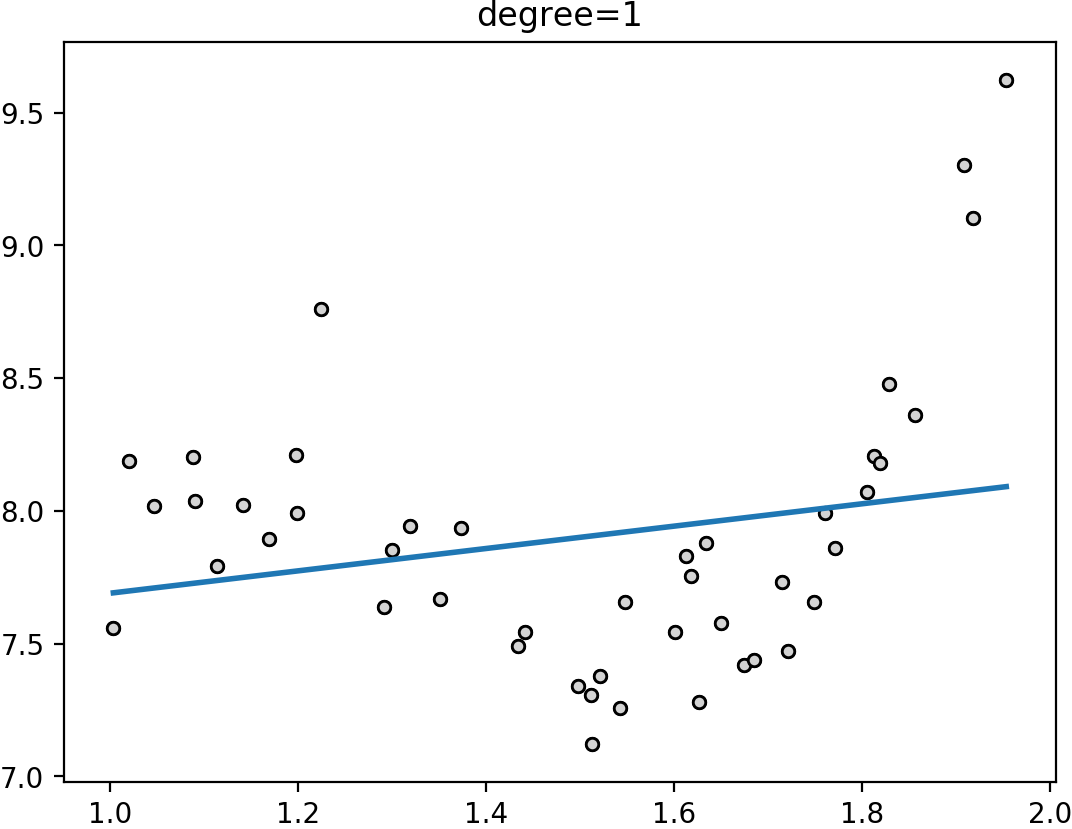
\includegraphics[width=\textwidth]{interp-pol-1.png}
    \end{figure}
\column{.33\textwidth}
\pause
    \begin{figure}
    \caption*{degree = 3 }
    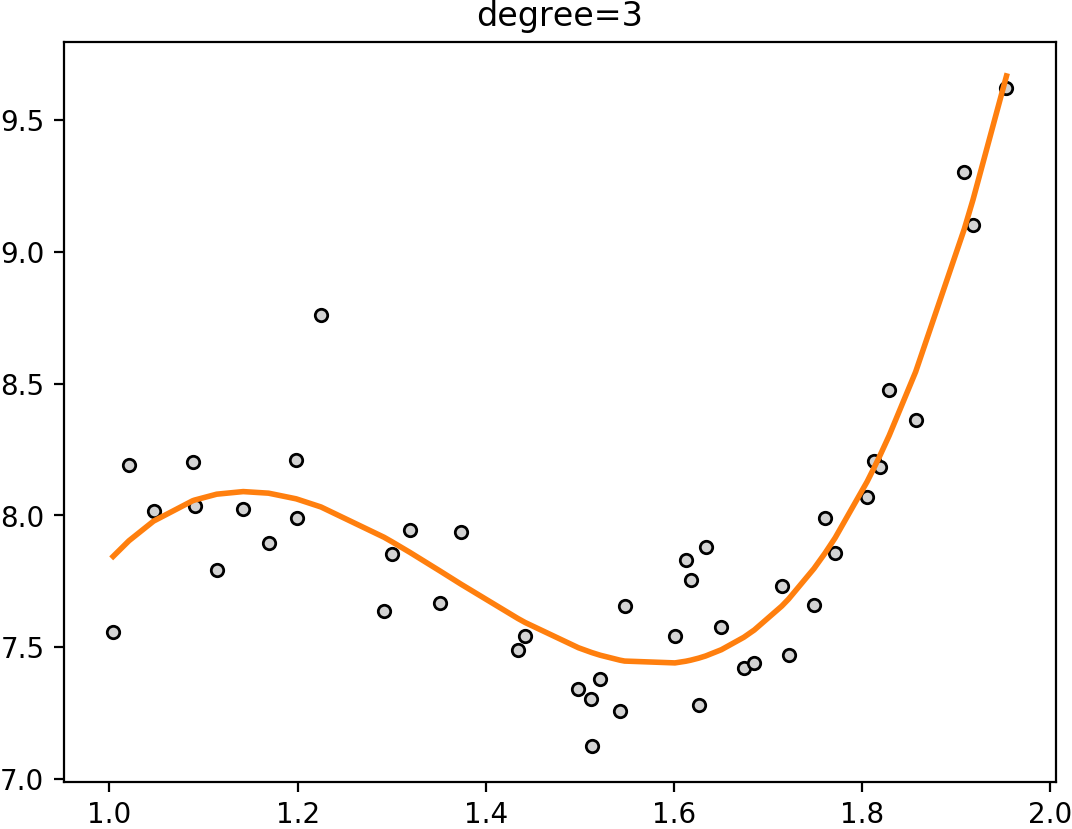
\includegraphics[width=\textwidth]{interp-pol-3.png}
    \end{figure}
\column{.33\textwidth}
\pause
    \begin{figure}
    \caption*{degree = 30 }
    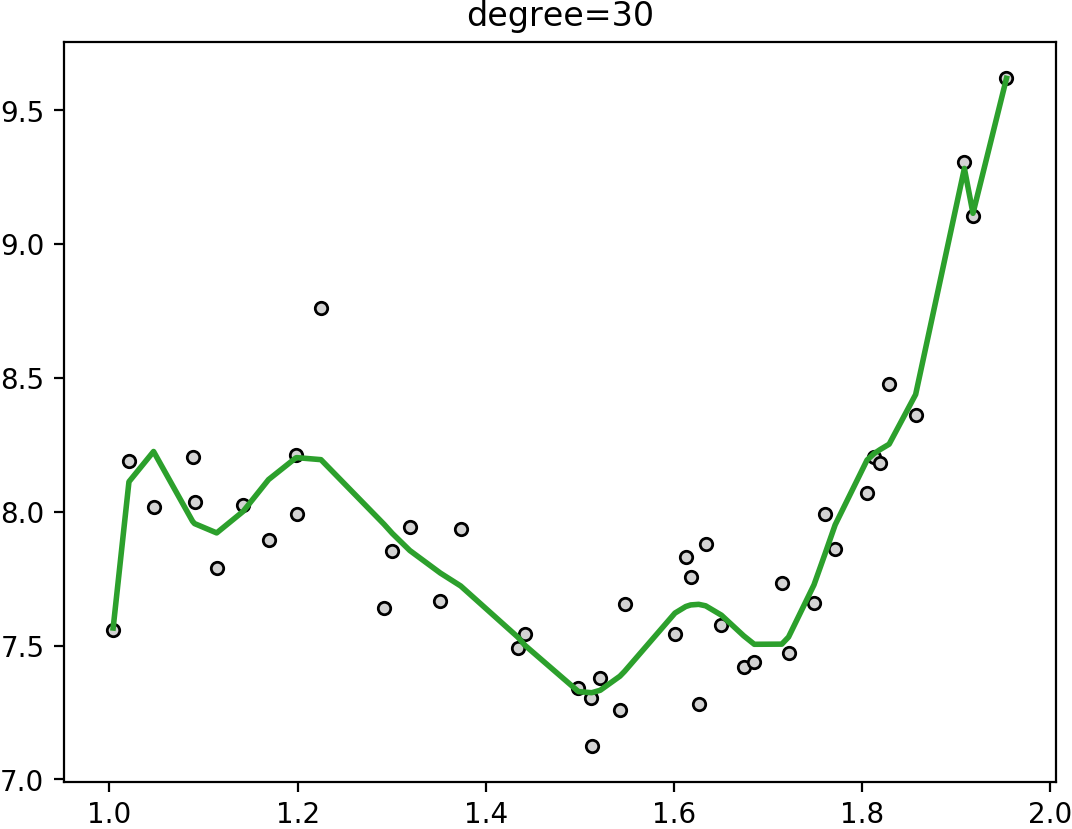
\includegraphics[width=\textwidth]{interp-pol-30.png}
    \end{figure}
 
\end{columns}
   
    \centering {
    \alert{What is the best model?}
    }
\end{frame}


%%%%%%%%%%%%%%%%%%%%
\begin{frame}{Train/Validation split}
\begin{block}{The idea}
Evaluate a score on a independent dataset
\end{block}
\pause
In our example we can randomly divide $(X,y)$ in two datasets:
\begin{itemize}
    \item The training dataset $X_{train},y_{train}$ used to fit the  model.
    \item The validation dataset $X_{val},y_{val}$ used to compute the score (e.g., correlation, mean-squared error)
\end{itemize}

    \begin{figure}
    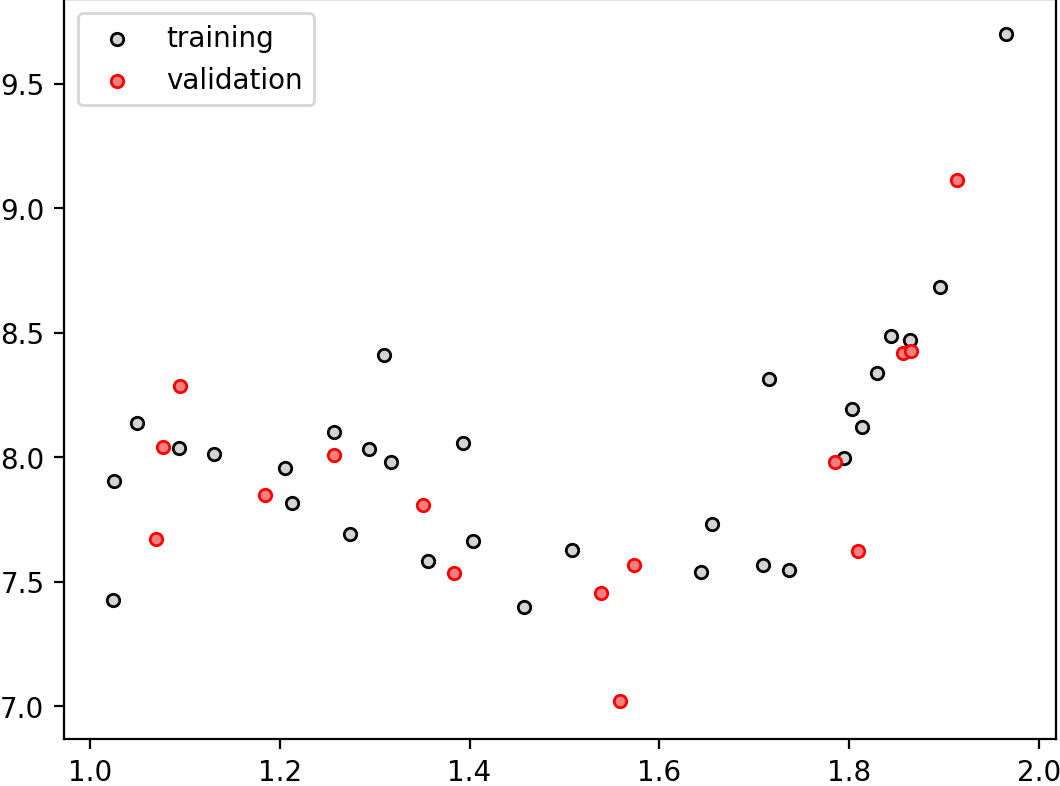
\includegraphics[width=.4\textwidth]{datasplit.png}
    \end{figure}

\end{frame}

%%%%%%%%%%%%%%%%%%%
\begin{frame}{Choice of the model}
\begin{columns}
\column{.5\textwidth}

    \begin{figure}
    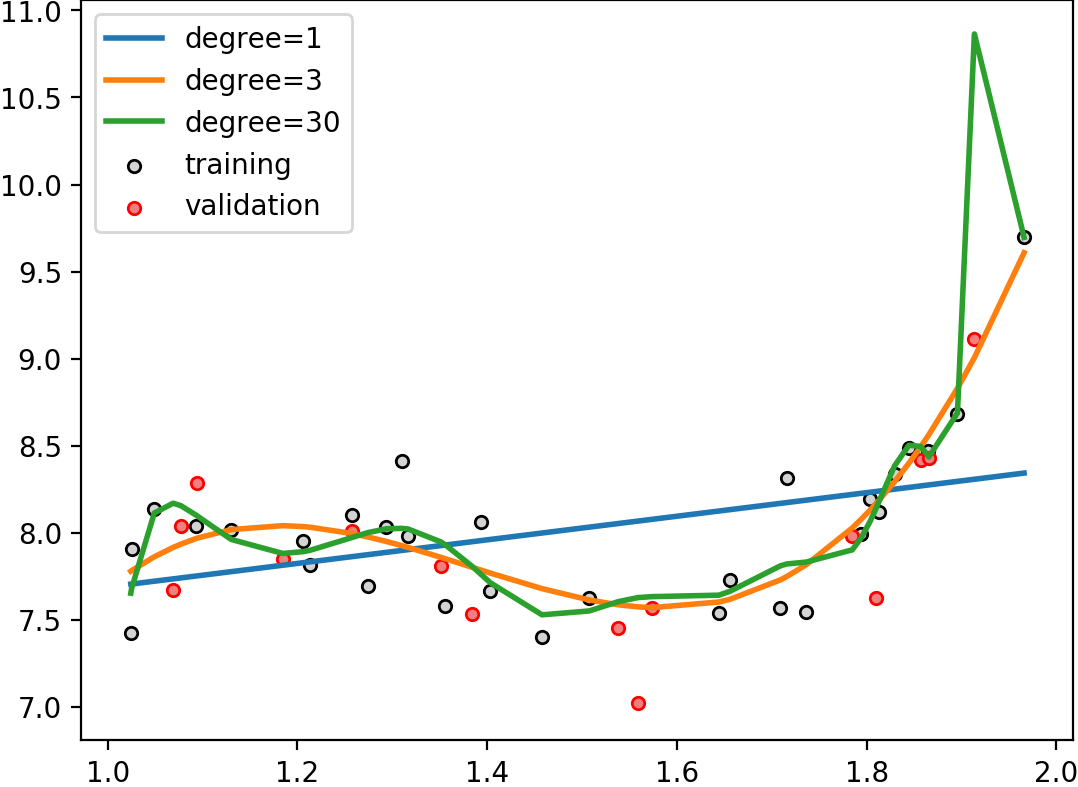
\includegraphics[width=\textwidth]{modelchoice.png}
    \end{figure}
\column{.5\textwidth}
Score: Mean Square Error (MSE)
\begin{table}
    \centering
    \begin{tabular}{c|c|c}
        Deg. & Train Score & Val. Score \\
        \hline
        1 & 0.17 & 0.23\\
        3 & 0.045 & 0.062\\
        30 & 0.035 & 0.27  \\
    \end{tabular}
    \end{table}
    %deg 1 ,score: val= 0.2283939842150192  , train= 0.167306864804612  , cv= 0.2768505679342689
%deg 3 ,score: val= 0.062492089527889656  , train= 0.04486320473714161  , cv= 0.05378120725339085
%deg 30 ,score: val= 0.27582336720042394  , train= 0.03473760406327127  , cv= 105306.65534552556
\end{columns}
\pause
   \begin{figure}
    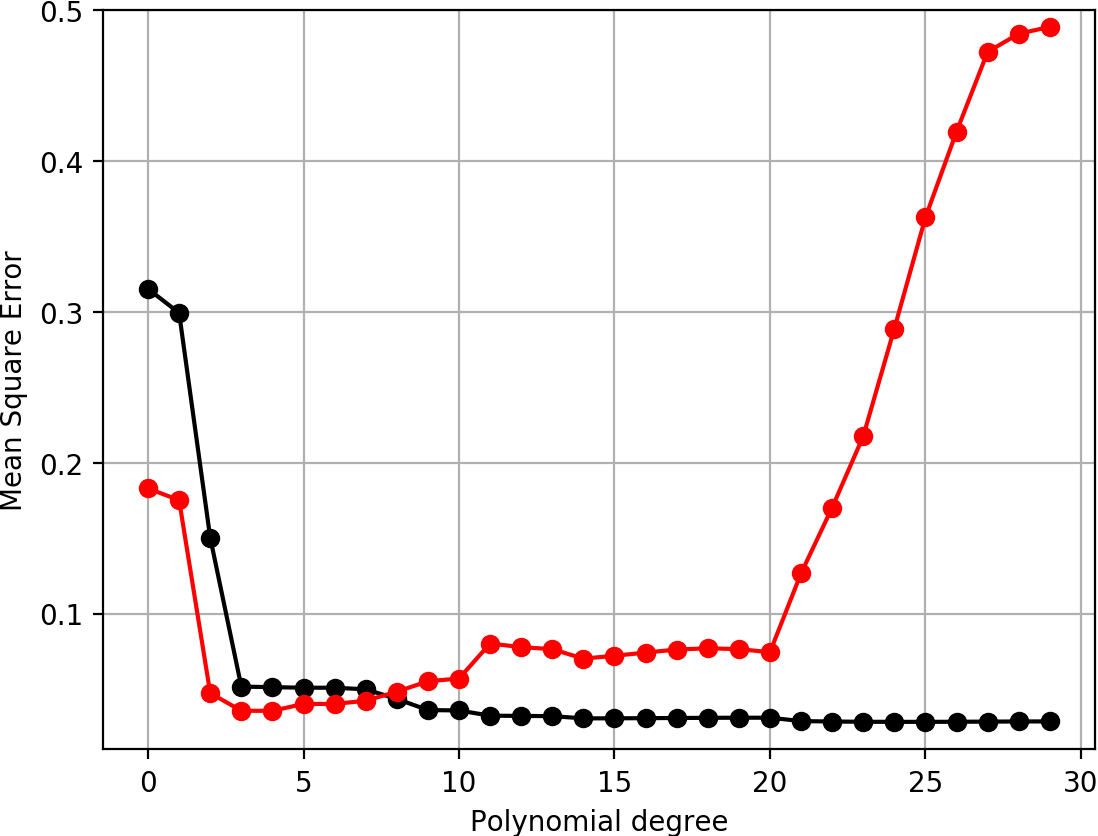
\includegraphics[width=.45\textwidth]{RMSE-deg-2scores.png}
    \end{figure}

\end{frame}

%%%%%%%%%%%%%%%%%%%%
\begin{frame}{Choice of the model}
\begin{block}{Polynomial regression}
$y=\theta_0 + \theta_1 x + \theta_2 x^2 + \cdots + \theta_d x^d = \sum_{i=0}^d \theta_i X^i$
\end{block}
\begin{columns}
\column{.33\textwidth}
    \begin{figure}
    \caption*{degree = 1 (linear)}
    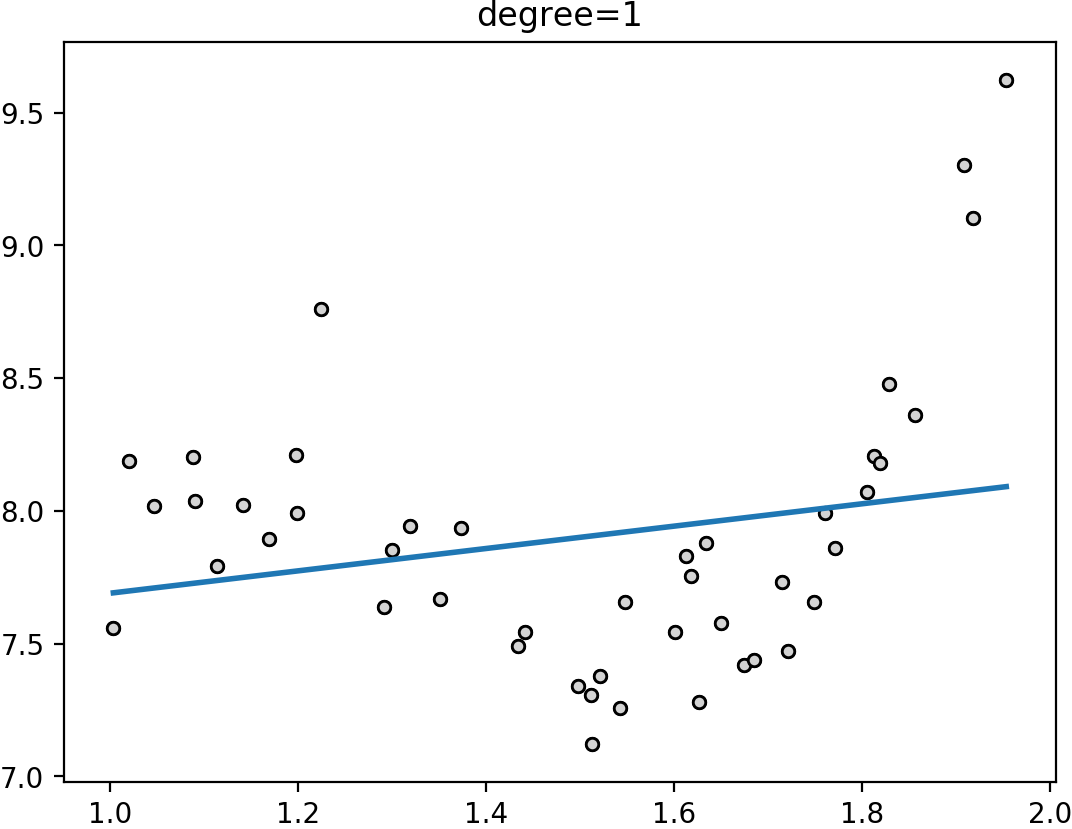
\includegraphics[width=\textwidth]{interp-pol-1.png}\\
        underfitting

    \end{figure}
\column{.33\textwidth}
    \begin{figure}
    \caption*{degree = 3 }
    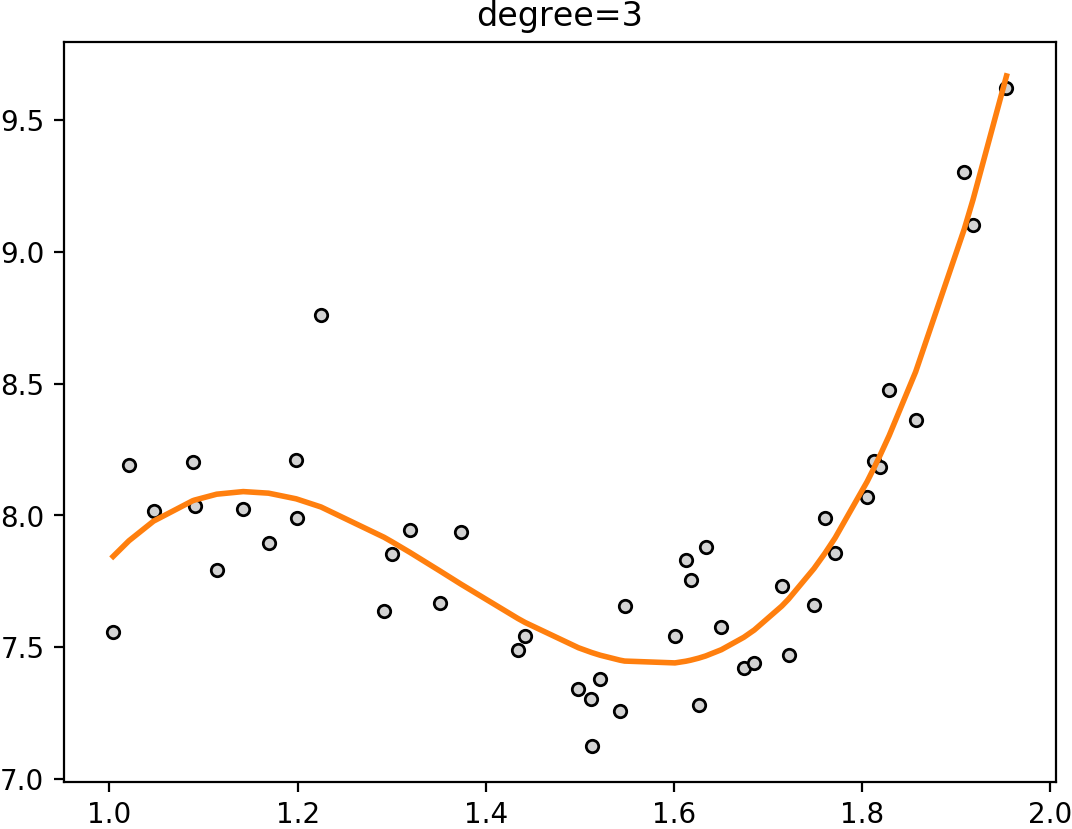
\includegraphics[width=\textwidth]{interp-pol-3.png}\\
        good fit

    \end{figure}
\column{.33\textwidth}
    \begin{figure}
    \caption*{degree = 30 }
    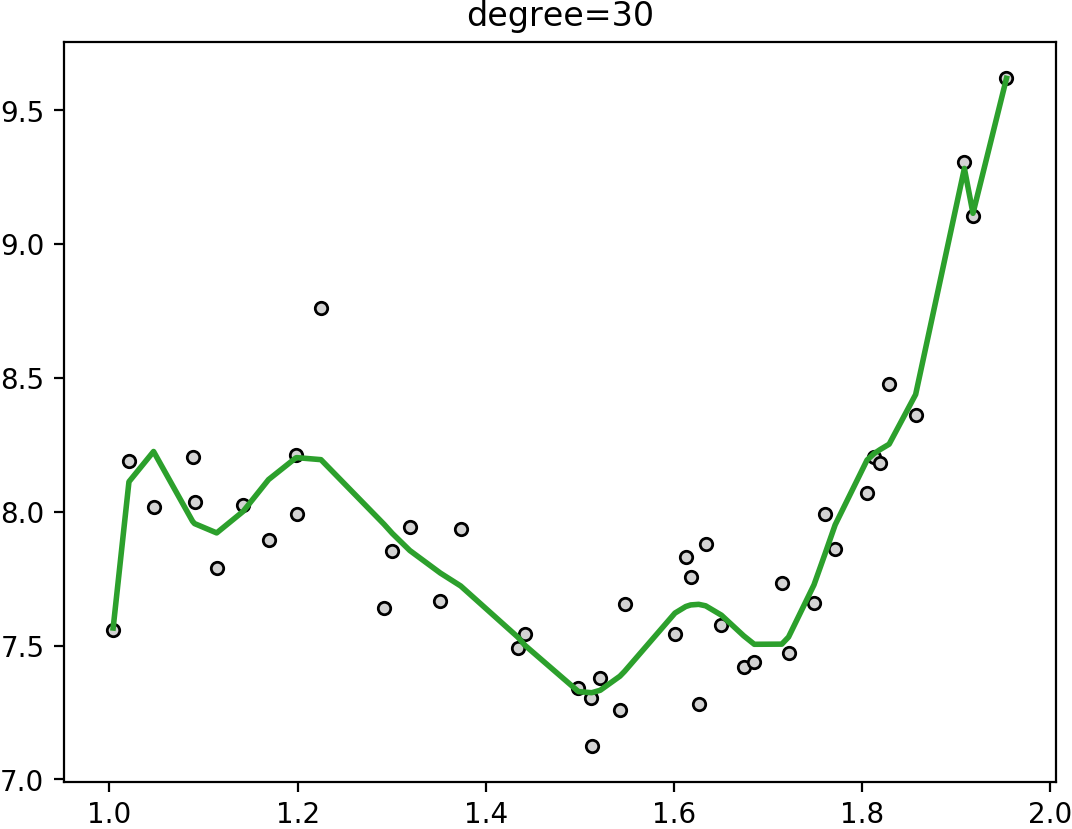
\includegraphics[width=\textwidth]{interp-pol-30.png}\\
        overfitting

    \end{figure}
 
\end{columns}

\end{frame}


%%%%%%%%%%%%%%%%%%%%
\begin{frame}{Train/Validation split}
     \begin{block}{Drawbacks}
\begin{itemize}
    \item drastically reduce the number of samples which can be used for learning the model
    \item Results  can depend on a particular random choice for the pair of (train, validation) sets.
\end{itemize}
\end{block}

\end{frame}
%%%%%%%%%%%%%%%%%%
\begin{frame}{More Robust: cross validation}
    \begin{block}{The idea}
    \begin{itemize}
\item Dividing the data in n folds, 
\item Learning n model (each time with a different training set),
\item Compute the mean score over n validation set.
\end{itemize}
\end{block}
   \begin{figure}
    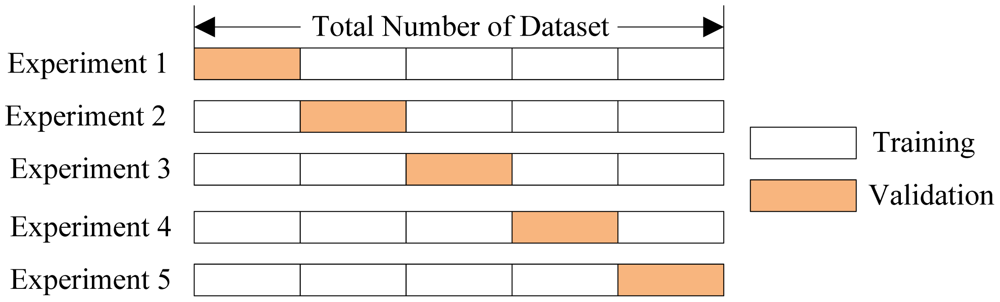
\includegraphics[width=\textwidth]{cv.png}
    \end{figure}

\end{frame}

%%%%%%%%%%%%%%%%%%%%
\begin{frame}{Cross-Validation}
\begin{columns}

\column{.3\textwidth}
\begin{table}
\footnotesize
    \centering
    \begin{tabular}{|c|c|}
    \hline
{\bf Fold} & {\bf MSE} \\
\hline
1 & 0.052 \\
2 & 0.043 \\
3 & 0.137 \\
4 & 0.025 \\
5 & 0.048 \\
6 & 0.144 \\
7 & 0.011 \\
8 & 0.025 \\
9 & 0.010 \\
10 & 0.028 \\
\hline
{\bf Mean} & {\bf 0.05} \\
        \hline


    \end{tabular}
    \end{table}
    
    \column{.7\textwidth}
   \begin{figure}
    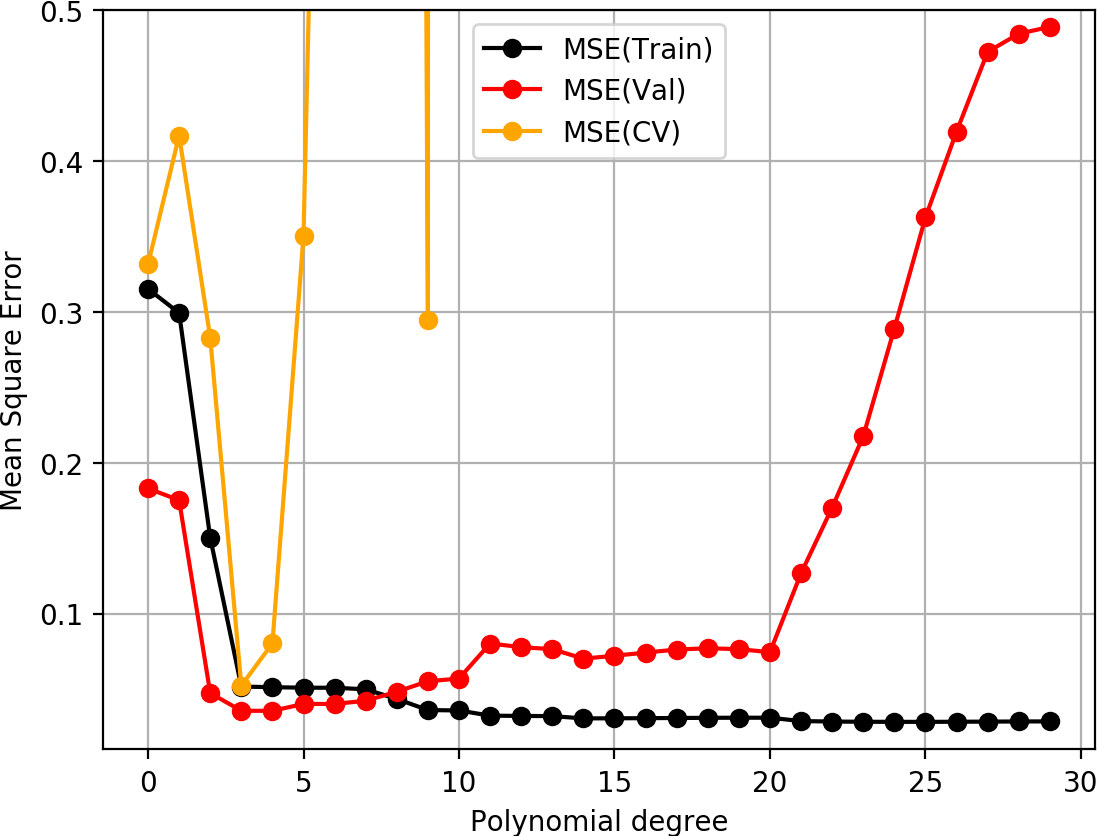
\includegraphics[width=\textwidth]{RMSE-deg-3scores.png}
    \end{figure}

\end{columns}

\end{frame}
%%%%%%%%%%%%%%%%
\begin{frame}{Wrapping up}
\begin{enumerate}[<+->]
    \item When applying machine learning techniques there are \alert{hyperparameters} to be determined (e.g., degree of the polynomial in polynomial regression).
    \item These \alert{hyperparameters}  can be determined by splitting the data into training/validation or by cross-validation.
    \item But then... the validation set was used to determine the best machine learning process
    \item To evaluate independanly the performance of our model, we should compute the score on a \alert{third independant dataset: The test dataset}.
    
\end{enumerate}
\end{frame}

\section{Case of auto-correlated data}

%%%%%%%%%%%%%%%%
\begin{frame}[fragile]{Random split}

\begin{itemize}[<+->]
\item A standard way to select the validation is to split randomly the dataset at a given proportion.\\
\textit{If 15\% of the point is in the validation set, each sample ${\bf x}_i$ has a probability of 15\% to be in the validation set}
\item It can be done using the sklearn python library
\begin{lstlisting}[language=Python]
from sklearn.model_selection import train_test_split

X_train, X_test, y_train, y_test = 
    train_test_split(X, y, test_size=0.15)
\end{lstlisting}
\item {\large \textcolor{red}{WARNING!}} It can lead to problems with auto-correlated data (e.g. pixels of an image, time series).\\
\alert {More exactly}: it leads to problem if the residual between the target and the model prediction (a.k.a. model error) is auto-correlated.
\end{itemize}
\end{frame}

%%%%%%%%%%%%%%%%
\begin{frame}{Illustration}
\begin{columns}

 \column{.3\textwidth}
   \begin{figure}
    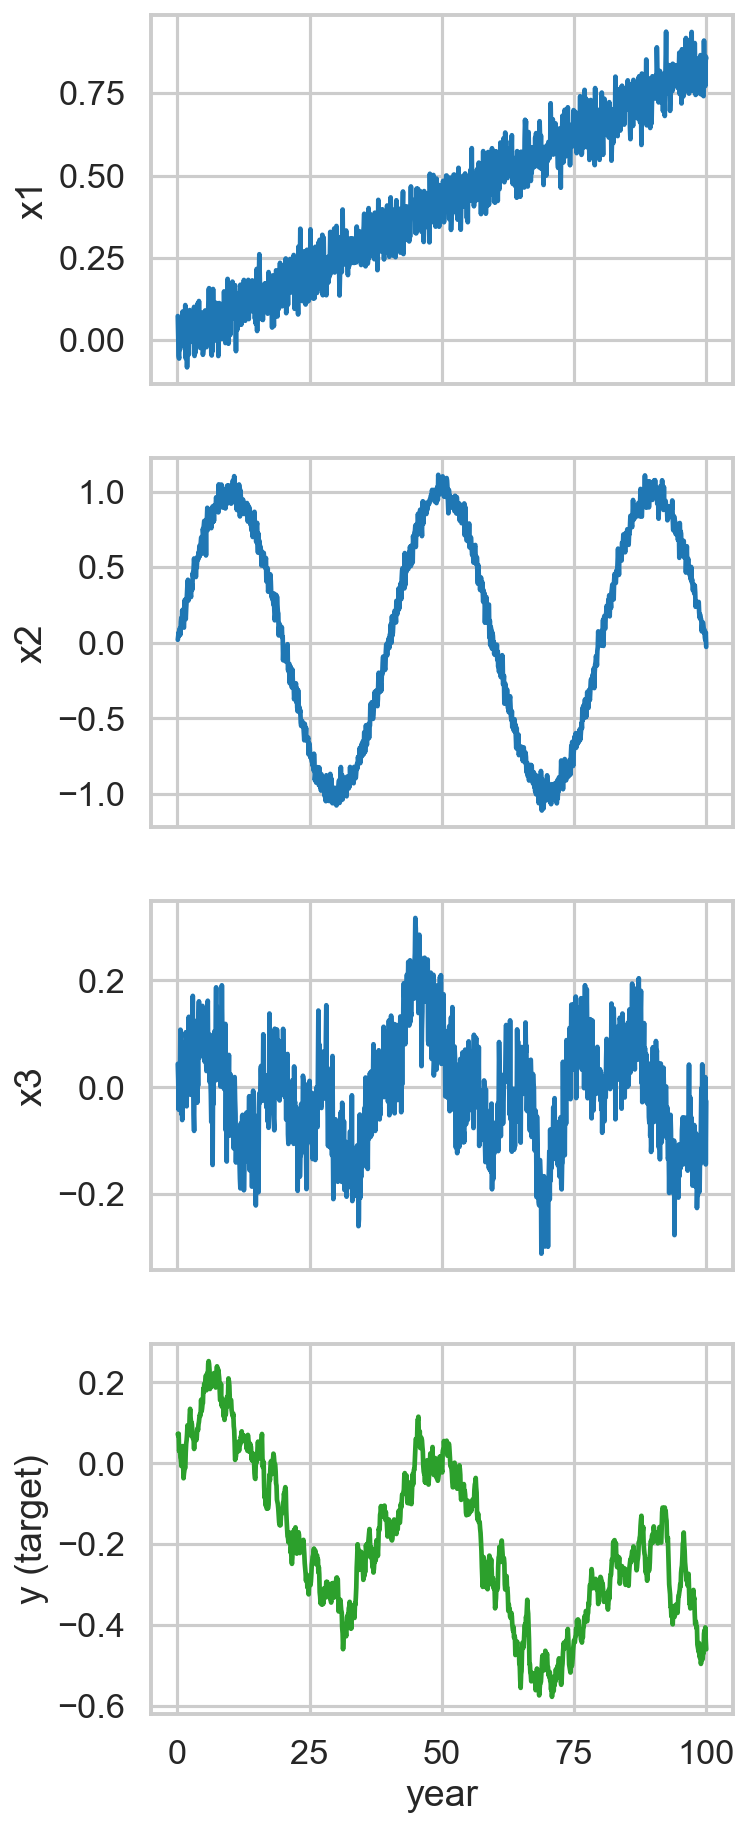
\includegraphics[width=\textwidth]{presentation/course-2/figs/leak_data.png}
    \end{figure}
    
    
\column{.7\textwidth}
\alert{Objective:} predict the target $y$ from the three features $x_1, x_2$ and $x_3$.\\
\vspace{2em}
Note: this is an artificial problem that have been created for the illustration. The true model is known:\\
$ y = -\frac{1}{2} x_1 + \frac{1}{5} x_2 +\frac{1}{5} x_3$

\pause
\begin{block}{Model and metric}
We will use a polynomial regression and chose the polynomial degree of the best nodel (in term of mean square error) from a validation set
\end{block}

\end{columns}

\end{frame}

%%%%%%%%%%%%%%%%
\begin{frame}{Result with random split}
\begin{columns}
\column{.5\textwidth}
   \begin{figure}
    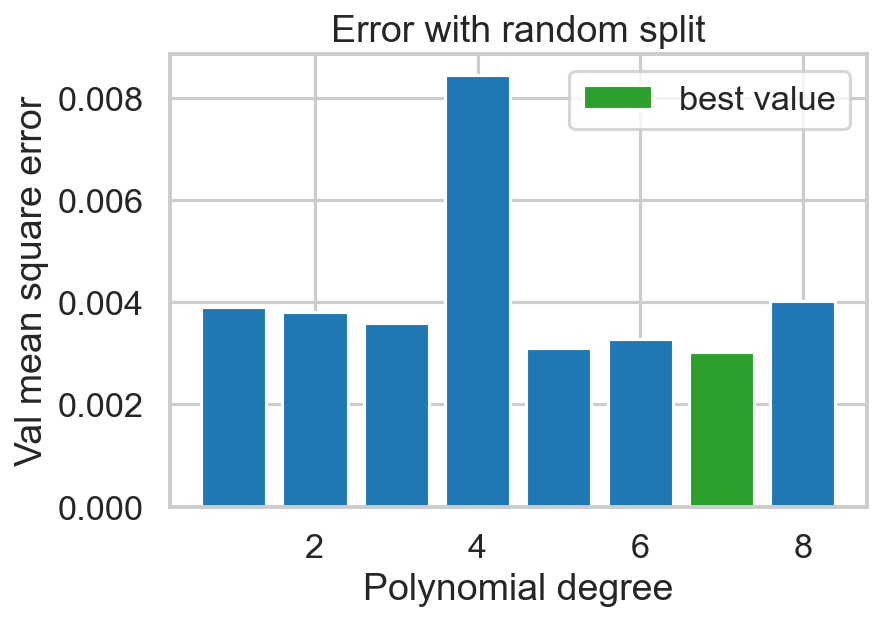
\includegraphics[width=.9\textwidth]{presentation/course-2/figs/leak_bar_random.png}
    \end{figure}
    
\column{.5\textwidth}
   \begin{figure}
    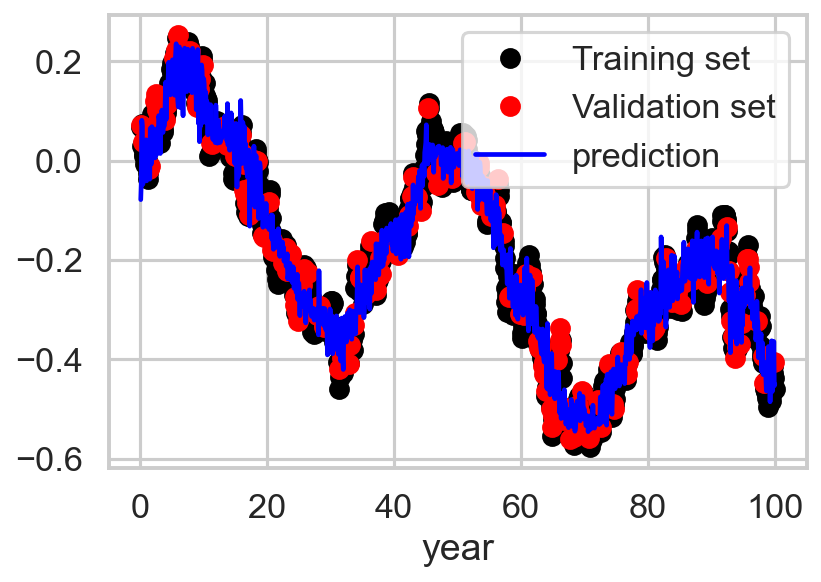
\includegraphics[width=.9\textwidth]{presentation/course-2/figs/leak_ts_random.png}
    \end{figure}
\end{columns}

   \begin{figure}
   \centering
   Can the model determine ($d=7$) generalize to new data? (year > 100)\\
   \pause
    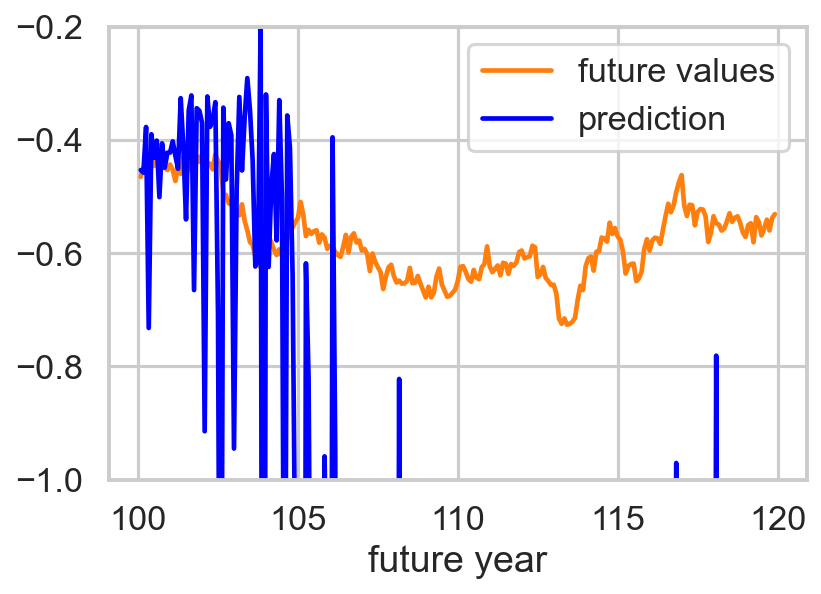
\includegraphics[width=.5\textwidth]{presentation/course-2/figs/leak_test_random.png}
    \end{figure}
\end{frame}


%%%%%%%%%%%%%%%%
\begin{frame}{One approach: block split}

\begin{columns}
\column{.5\textwidth}
  \begin{figure}
  \centering
  Random split (15\%)
    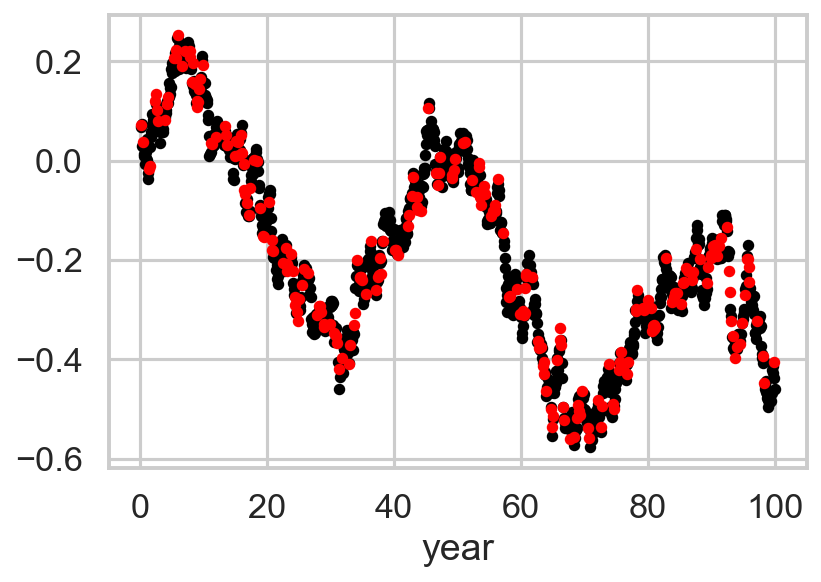
\includegraphics[width=\textwidth]{presentation/course-2/figs/leak_ts_random_nopred.png}
    \end{figure}
    \column{.5\textwidth}
  \begin{figure}
  \centering
  Block split (15\%)
    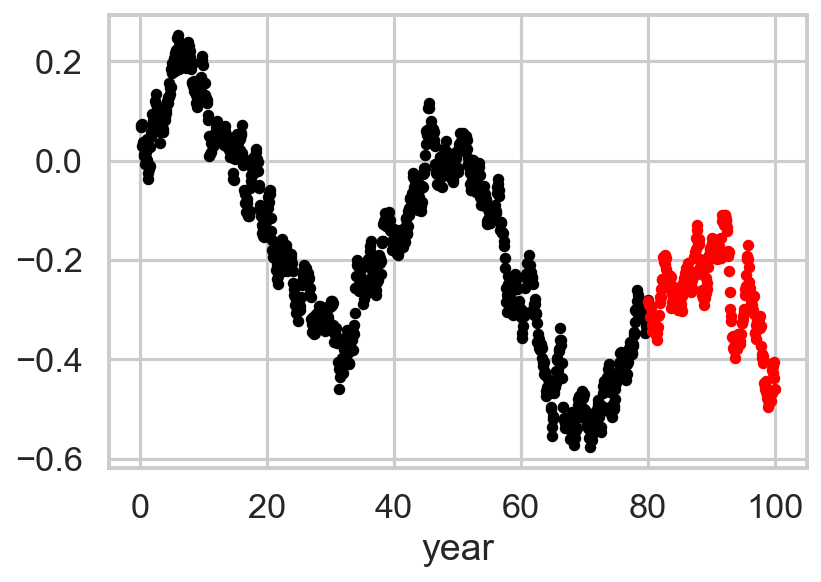
\includegraphics[width=\textwidth]{presentation/course-2/figs/leak_ts_block_nopred.png}
    \end{figure}
\end{columns}
\end{frame}
%%%%%%%%%%%%%%%%
\begin{frame}{Result with block split}
\begin{columns}
\column{.5\textwidth}
   \begin{figure}
    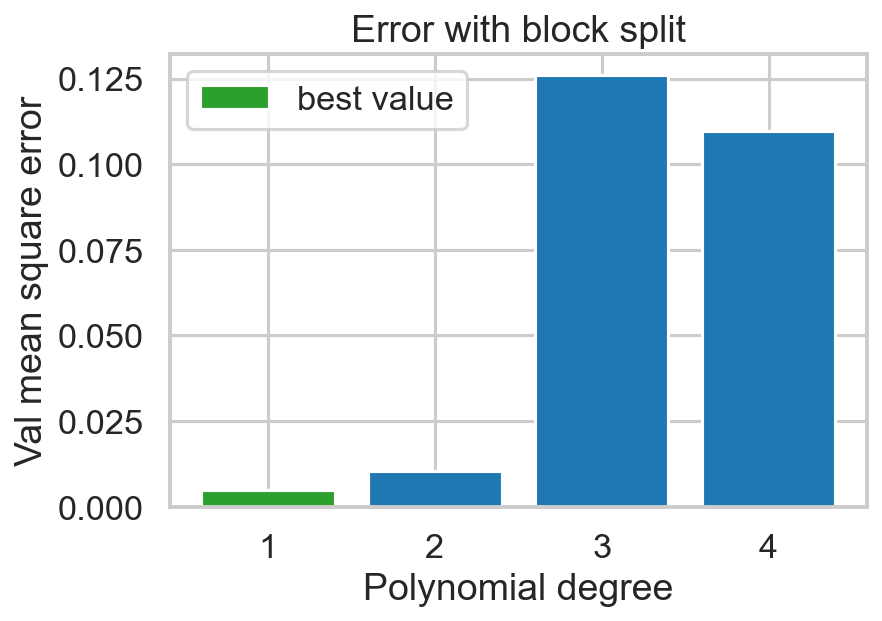
\includegraphics[width=.9\textwidth]{presentation/course-2/figs/leak_bar_block.png}
    \end{figure}
    
\column{.5\textwidth}
   \begin{figure}
    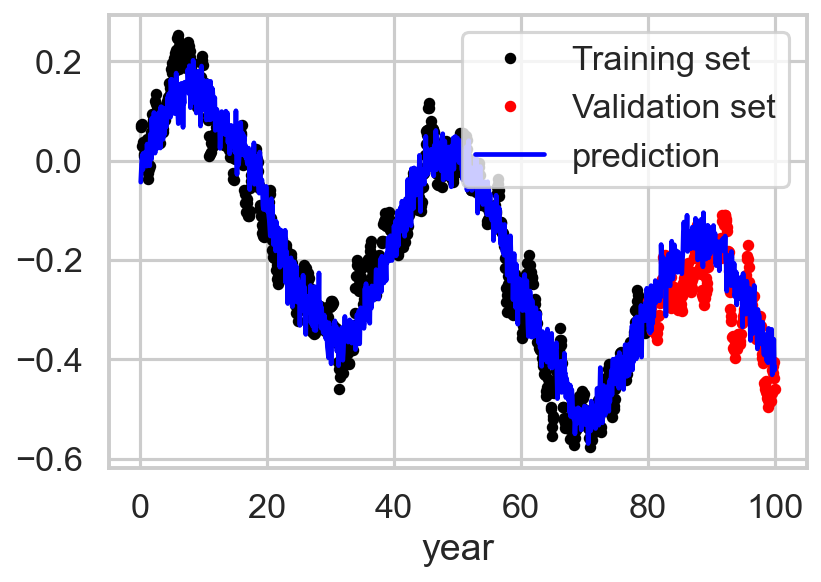
\includegraphics[width=.9\textwidth]{presentation/course-2/figs/leak_ts_block.png}
    \end{figure}
\end{columns}

   \begin{figure}
   \centering
   Can the model determine ($d=1$) generalize to new data? (year > 100)\\
   \pause
    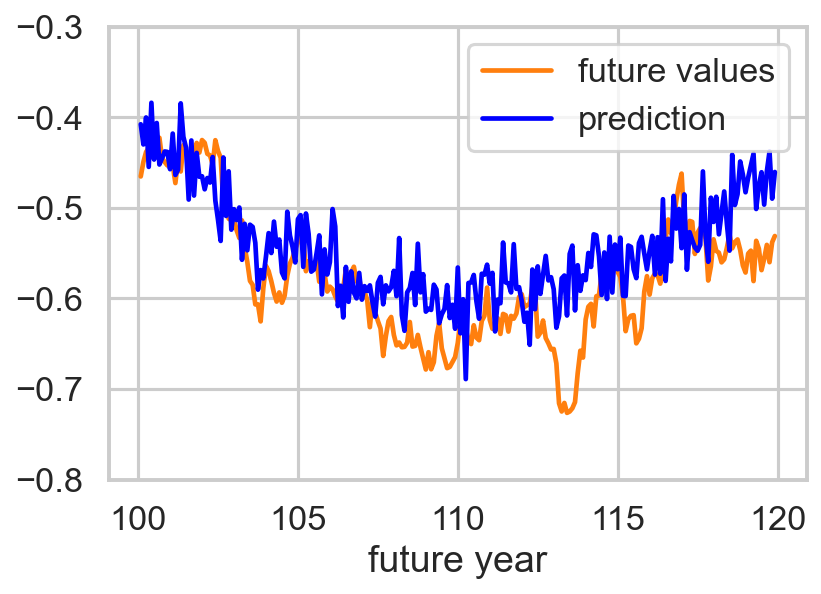
\includegraphics[width=.5\textwidth]{presentation/course-2/figs/leak_test_block.png}
    \end{figure}
\end{frame}
\section{L1/L2 regularization}

\begin{frame}
\frametitle{Example of a non-linear relationship}
\begin{figure}
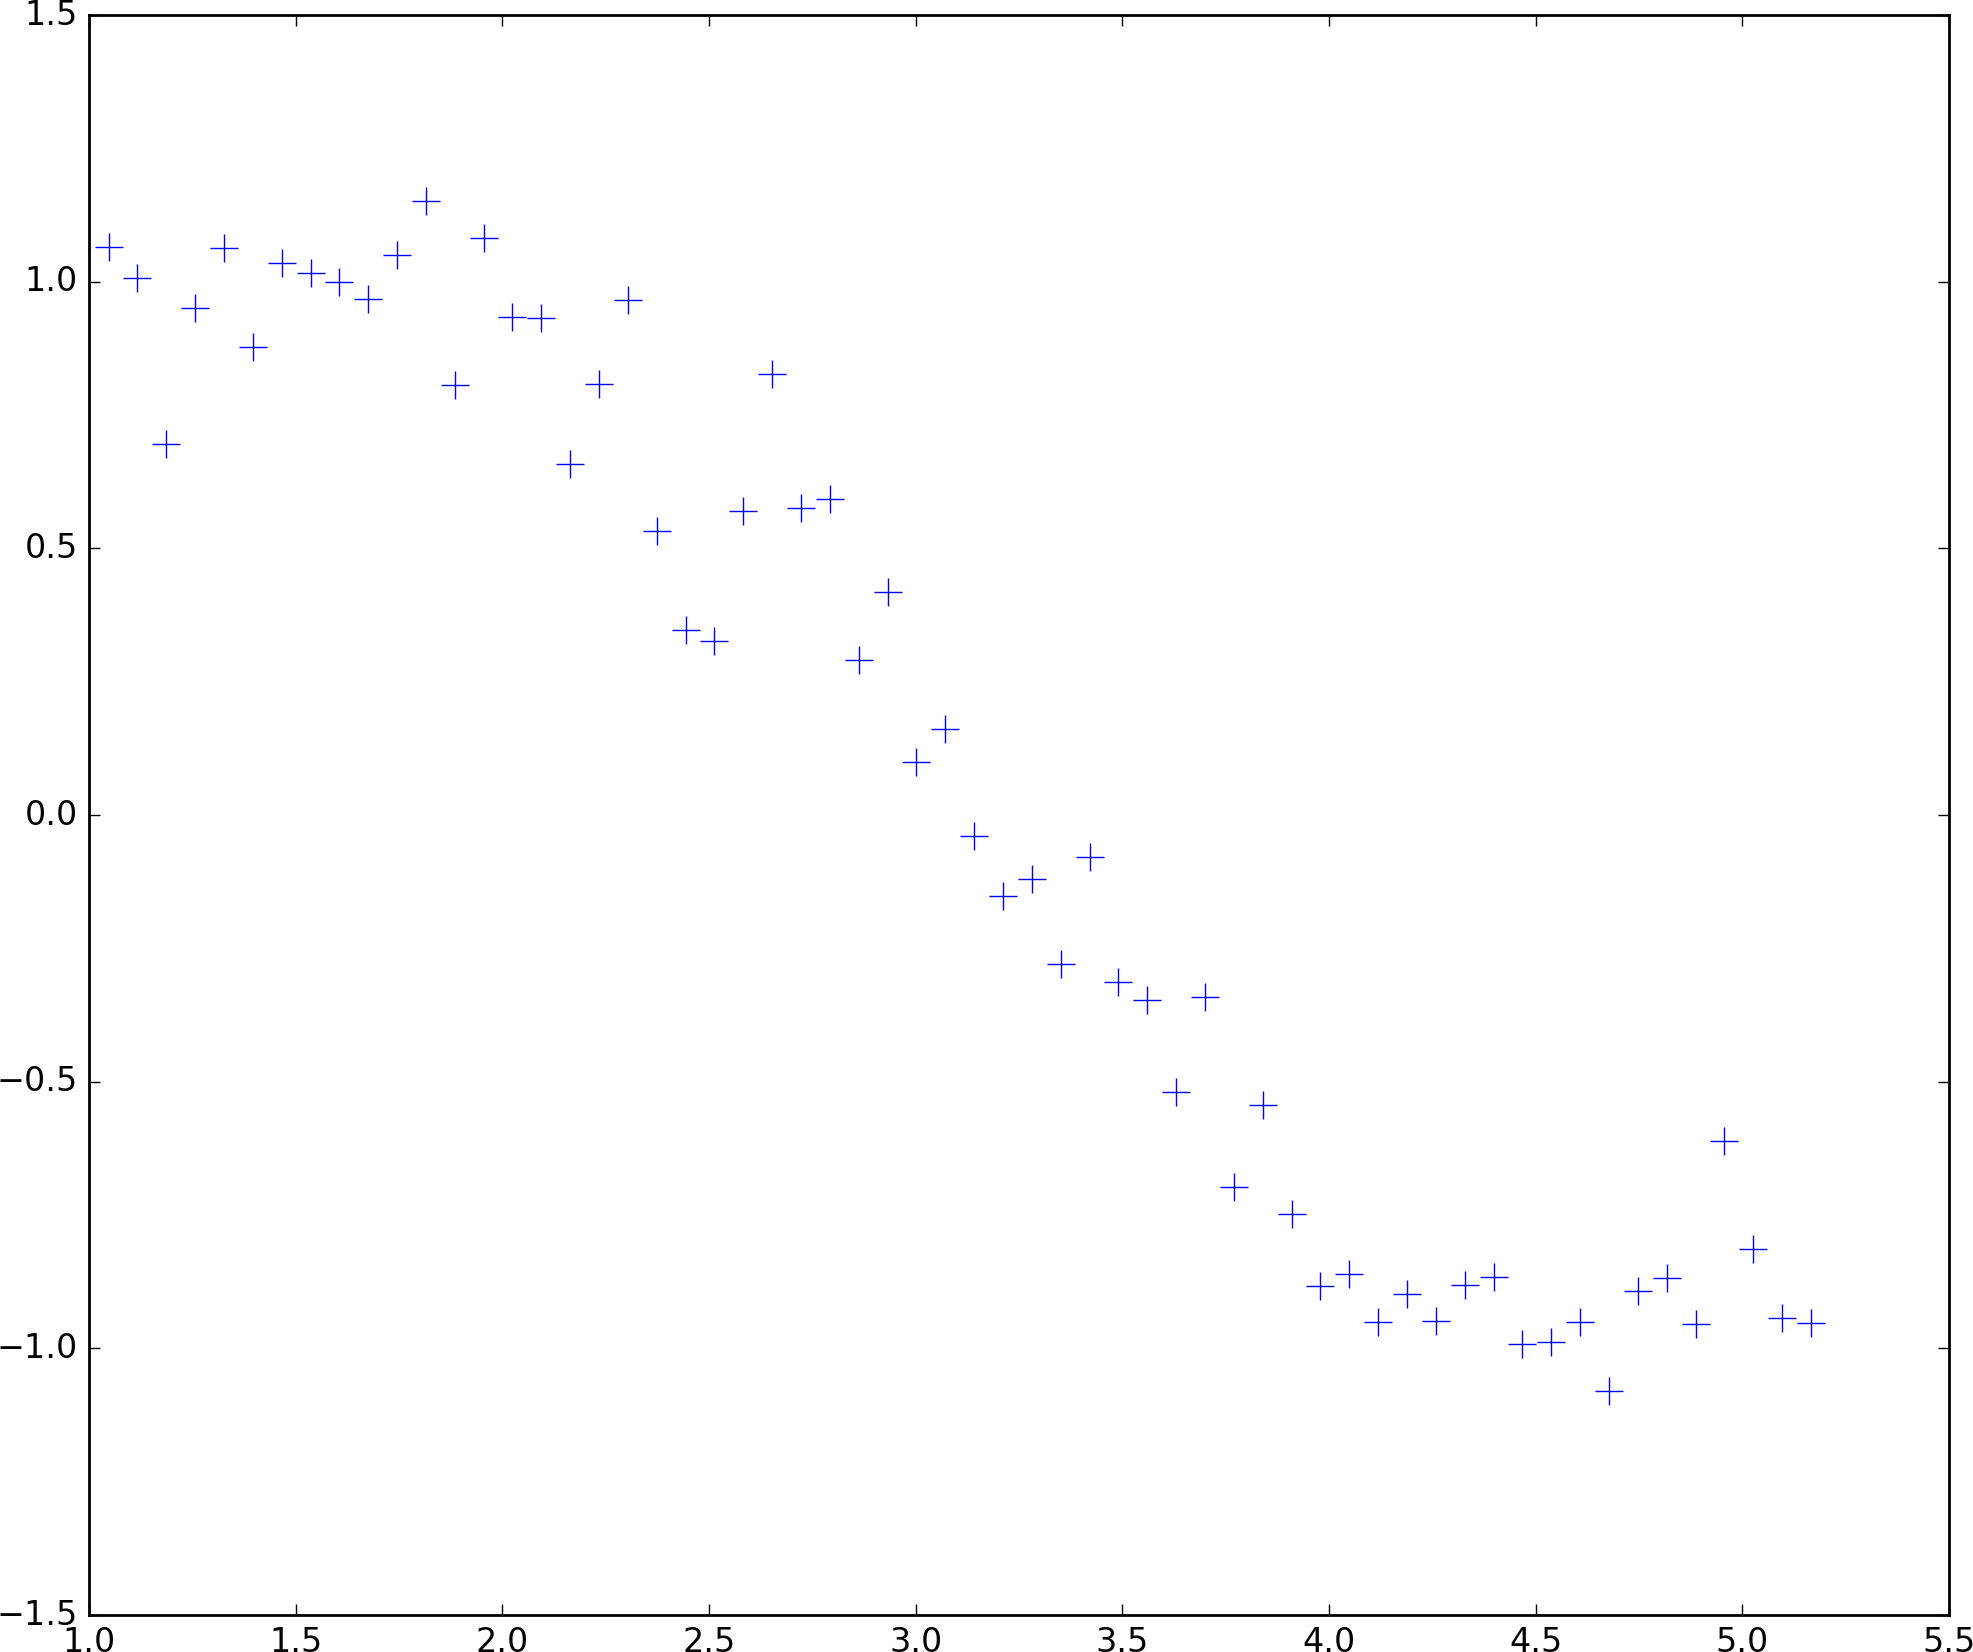
\includegraphics[height=0.55\textheight]{./scatter.png}
\end{figure}
\begin{block}{An idea}
We could take an polynomial hypothesis model:
$$
h_{\bm{\theta}}(x) = \theta_0 x^0 + \theta_1 x^1 + \ldots + \theta_p x^p
$$
\end{block}
\end{frame}
%%%%%%%%%%%%%%%%%%%%%
\begin{frame}
\frametitle{Example}
$\{(x_1,y_1),\ldots,(x_n,y_n)\}$ is the training dataset.

For a given polynomial degree $p$, parameters $\bm{\theta}$ are determined minimizing the 
least-mean square cost function:
$$
J(\bm{\theta}) = \frac{1}{n} \sum (y_i - h_{\bm{\theta}}(x_i))^2
$$
with $h_{\bm{\theta}}(x) = \theta_0 x^0 + \theta_1 x^1 + \ldots + \theta_p x^p$
\begin{itemize}[<+->]
\item It can be determined using a gradient descent method
\item If the degree of the polynomial $p=1$, it is a simple linear regression
\end{itemize}
\end{frame}
%%%%%%%%%%%%%%%%%%%%%
\begin{frame}
\frametitle{A first result}
\vspace{-2em}
\begin{columns}[t]
\column{.5\textwidth}
\begin{figure}
$p=1$ (linear regression)\\
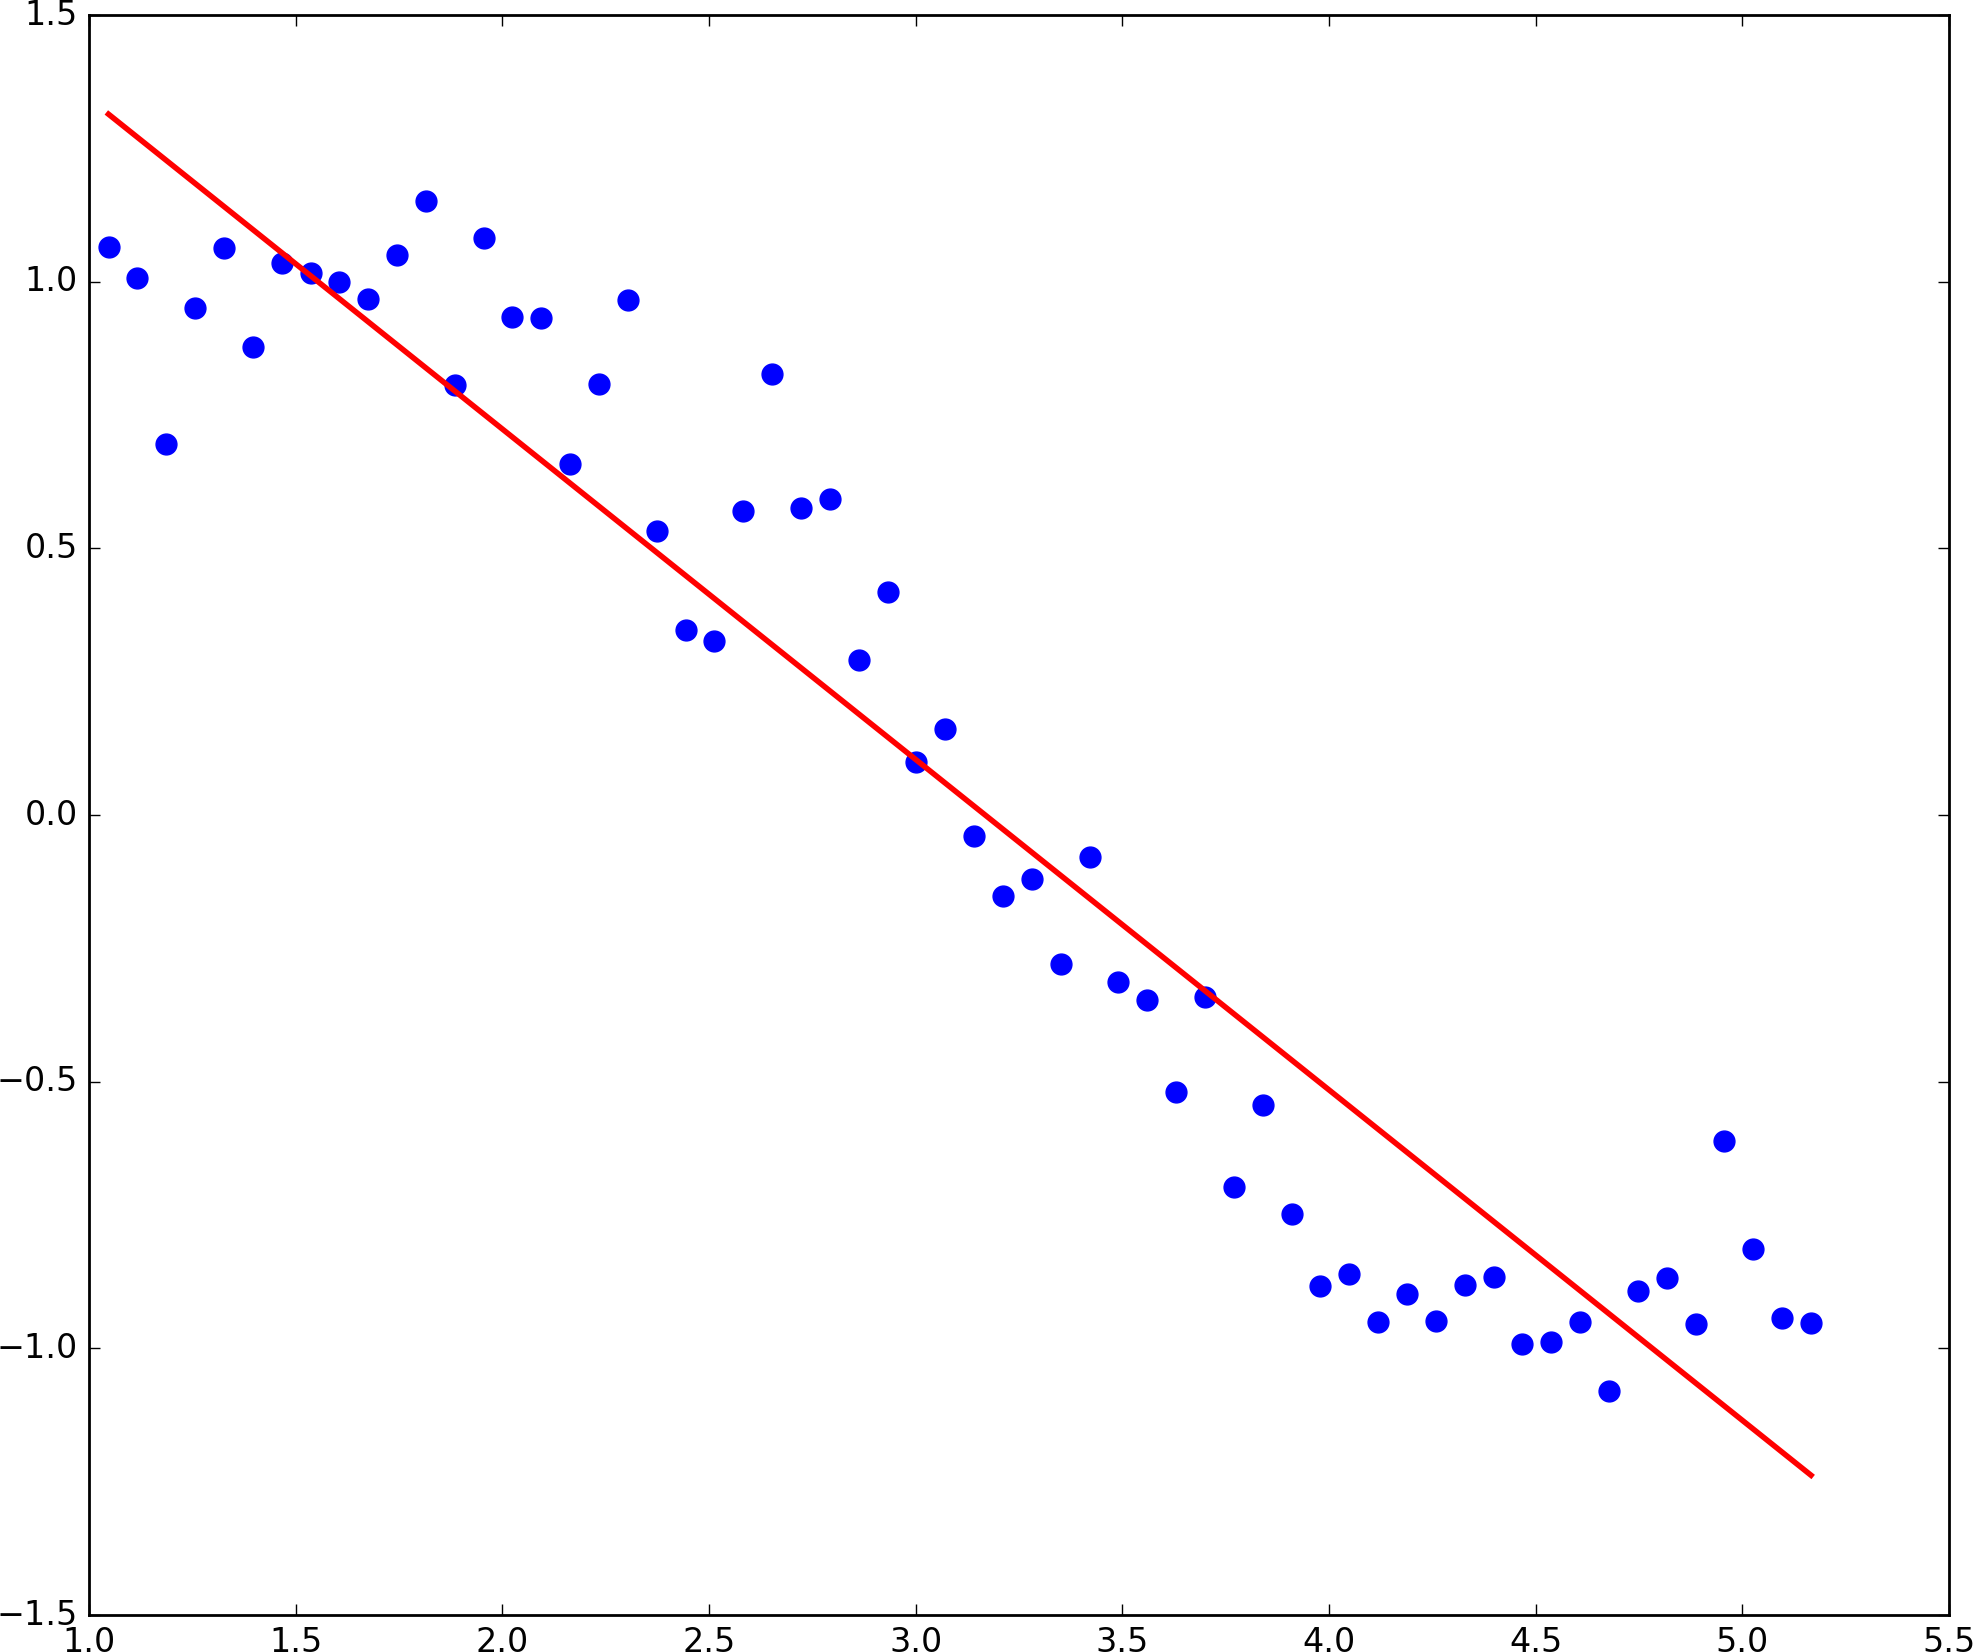
\includegraphics[width=0.99\textwidth]{./linreg_pow1.png}
\end{figure}
\column{.5\textwidth}
\begin{figure}
residuals\\
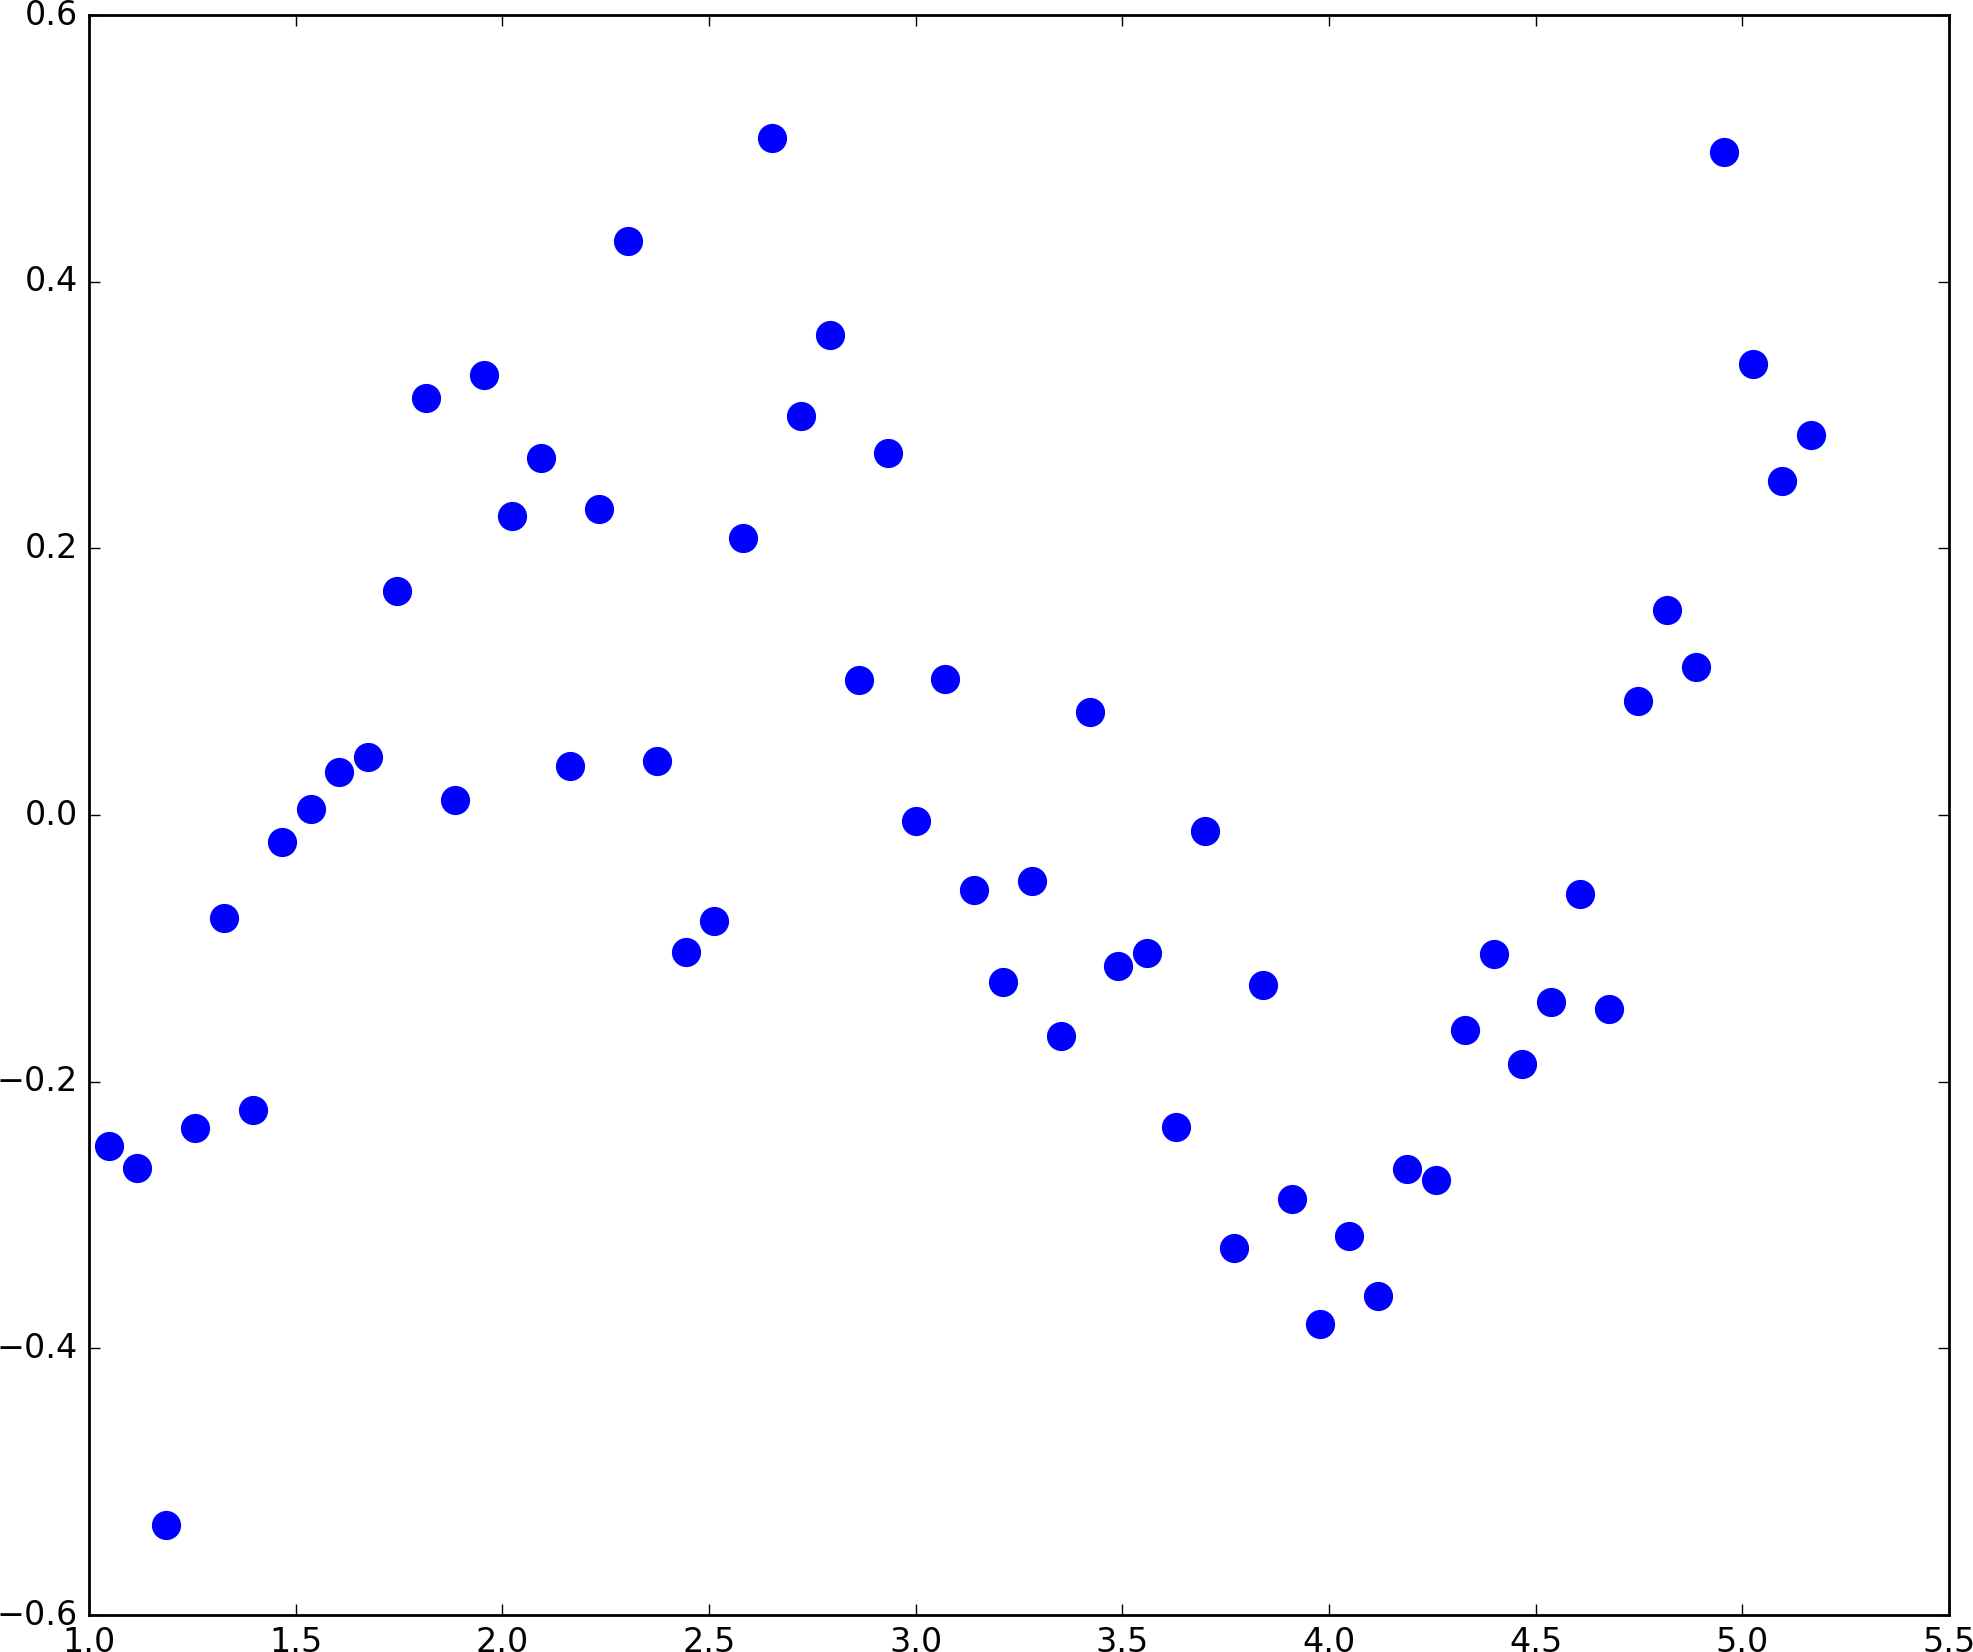
\includegraphics[width=0.99\textwidth]{./residuals.png}
\end{figure}

\end{columns}
\begin{block}{Prediction error}
$$
\text{err} = \frac{1}{n}\sum \text{res}^2 = 5.46e-2
$$
\end{block}

\end{frame}
%%%%%%%%%%%%%%%%%%%%%
\begin{frame}
\frametitle{Increasing the polynomial degree ?}
\begin{columns}
\column{.5\textwidth}
\begin{figure}
$p=3$ (cubic regression)\\
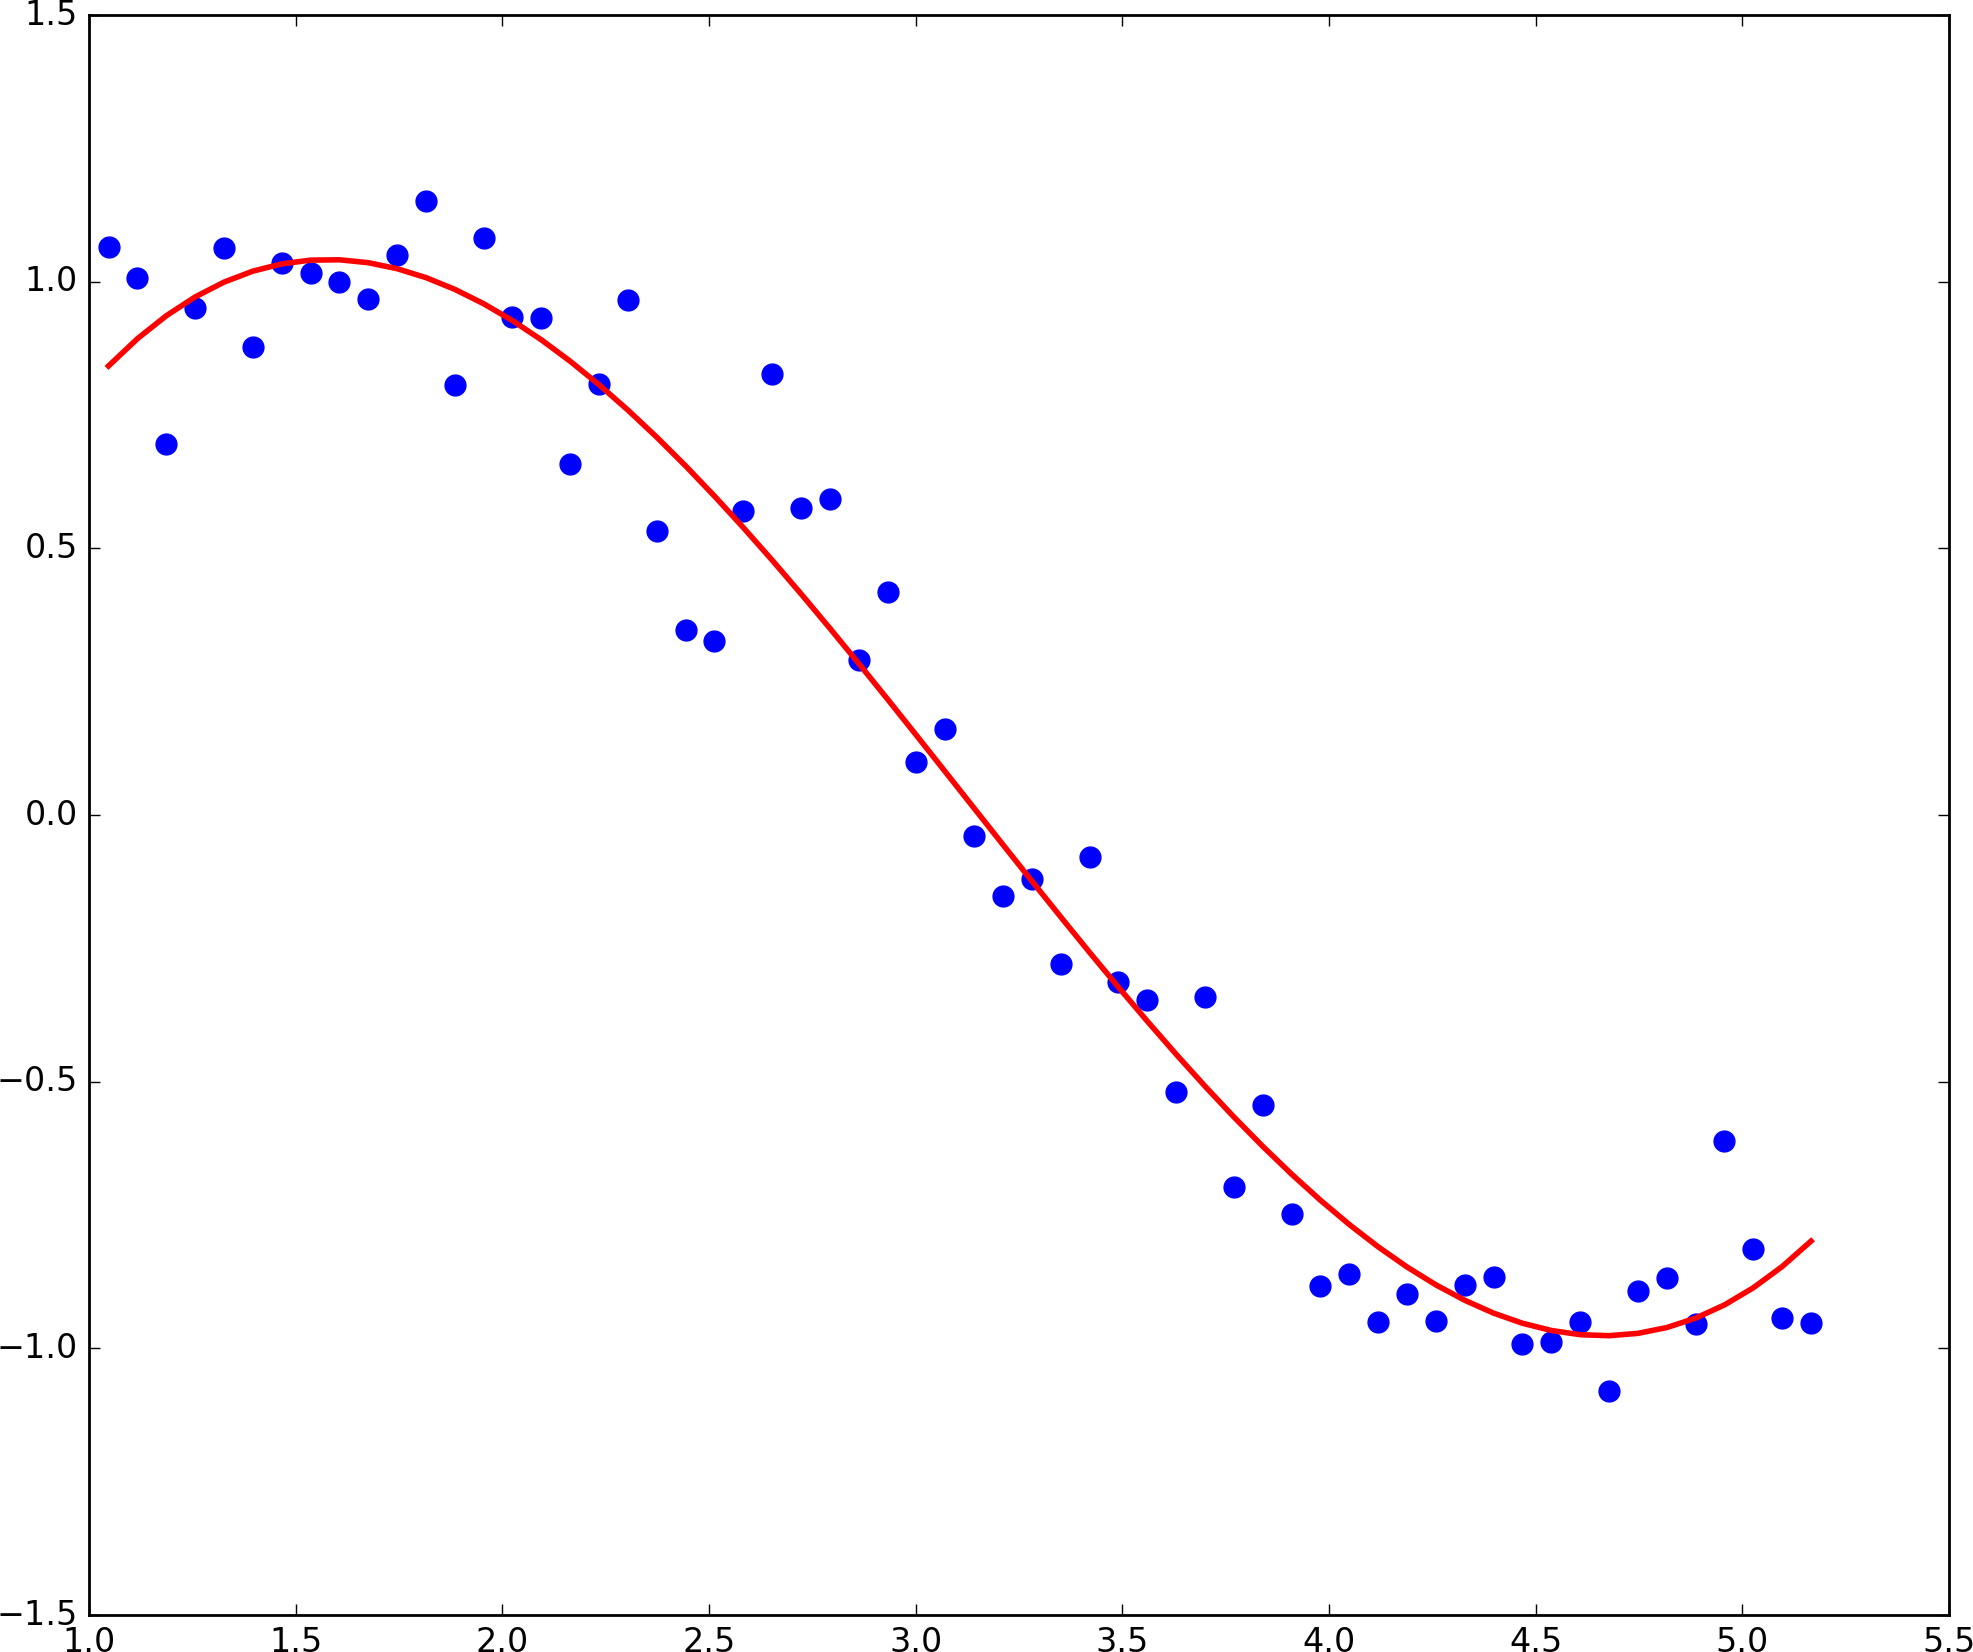
\includegraphics[width=0.99\textwidth]{./linreg_pow3.png}
\end{figure}
\column{.5\textwidth}
\begin{block}{Prediction error}
$$
\text{err} = \frac{1}{n}\sum \text{res}^2 = 1.80e-2
$$
\end{block}
\end{columns}
\end{frame}


%%%%%%%%%%%%%%%%%%%%%
\begin{frame}
\frametitle{Is it different from the linear regression ?}
Let's consider :
$$
\bm{x} = 
\begin{pmatrix}
1 \\
x^1 \\
x^2 \\
\vdots \\
x^p
\end{pmatrix}
$$
then
$$
h_{\bm{\theta}}(x) = \theta_0  + \theta_1 x^1 + \ldots + \theta_p x^p = \bm{\theta}^T \bm{x}
$$
\begin{alertblock}{}
By extending a scalar predictor to a vector,
polynomial regression is equivalent to linear regression.
\end{alertblock}

\end{frame}

%%%%%%%%%%%%%%%%%%%%%
\begin{frame}
\frametitle{Increasing the degree ?}
\begin{columns}
\column{.33\textwidth}
\vspace{-2em}
\begin{figure}
$p=1$
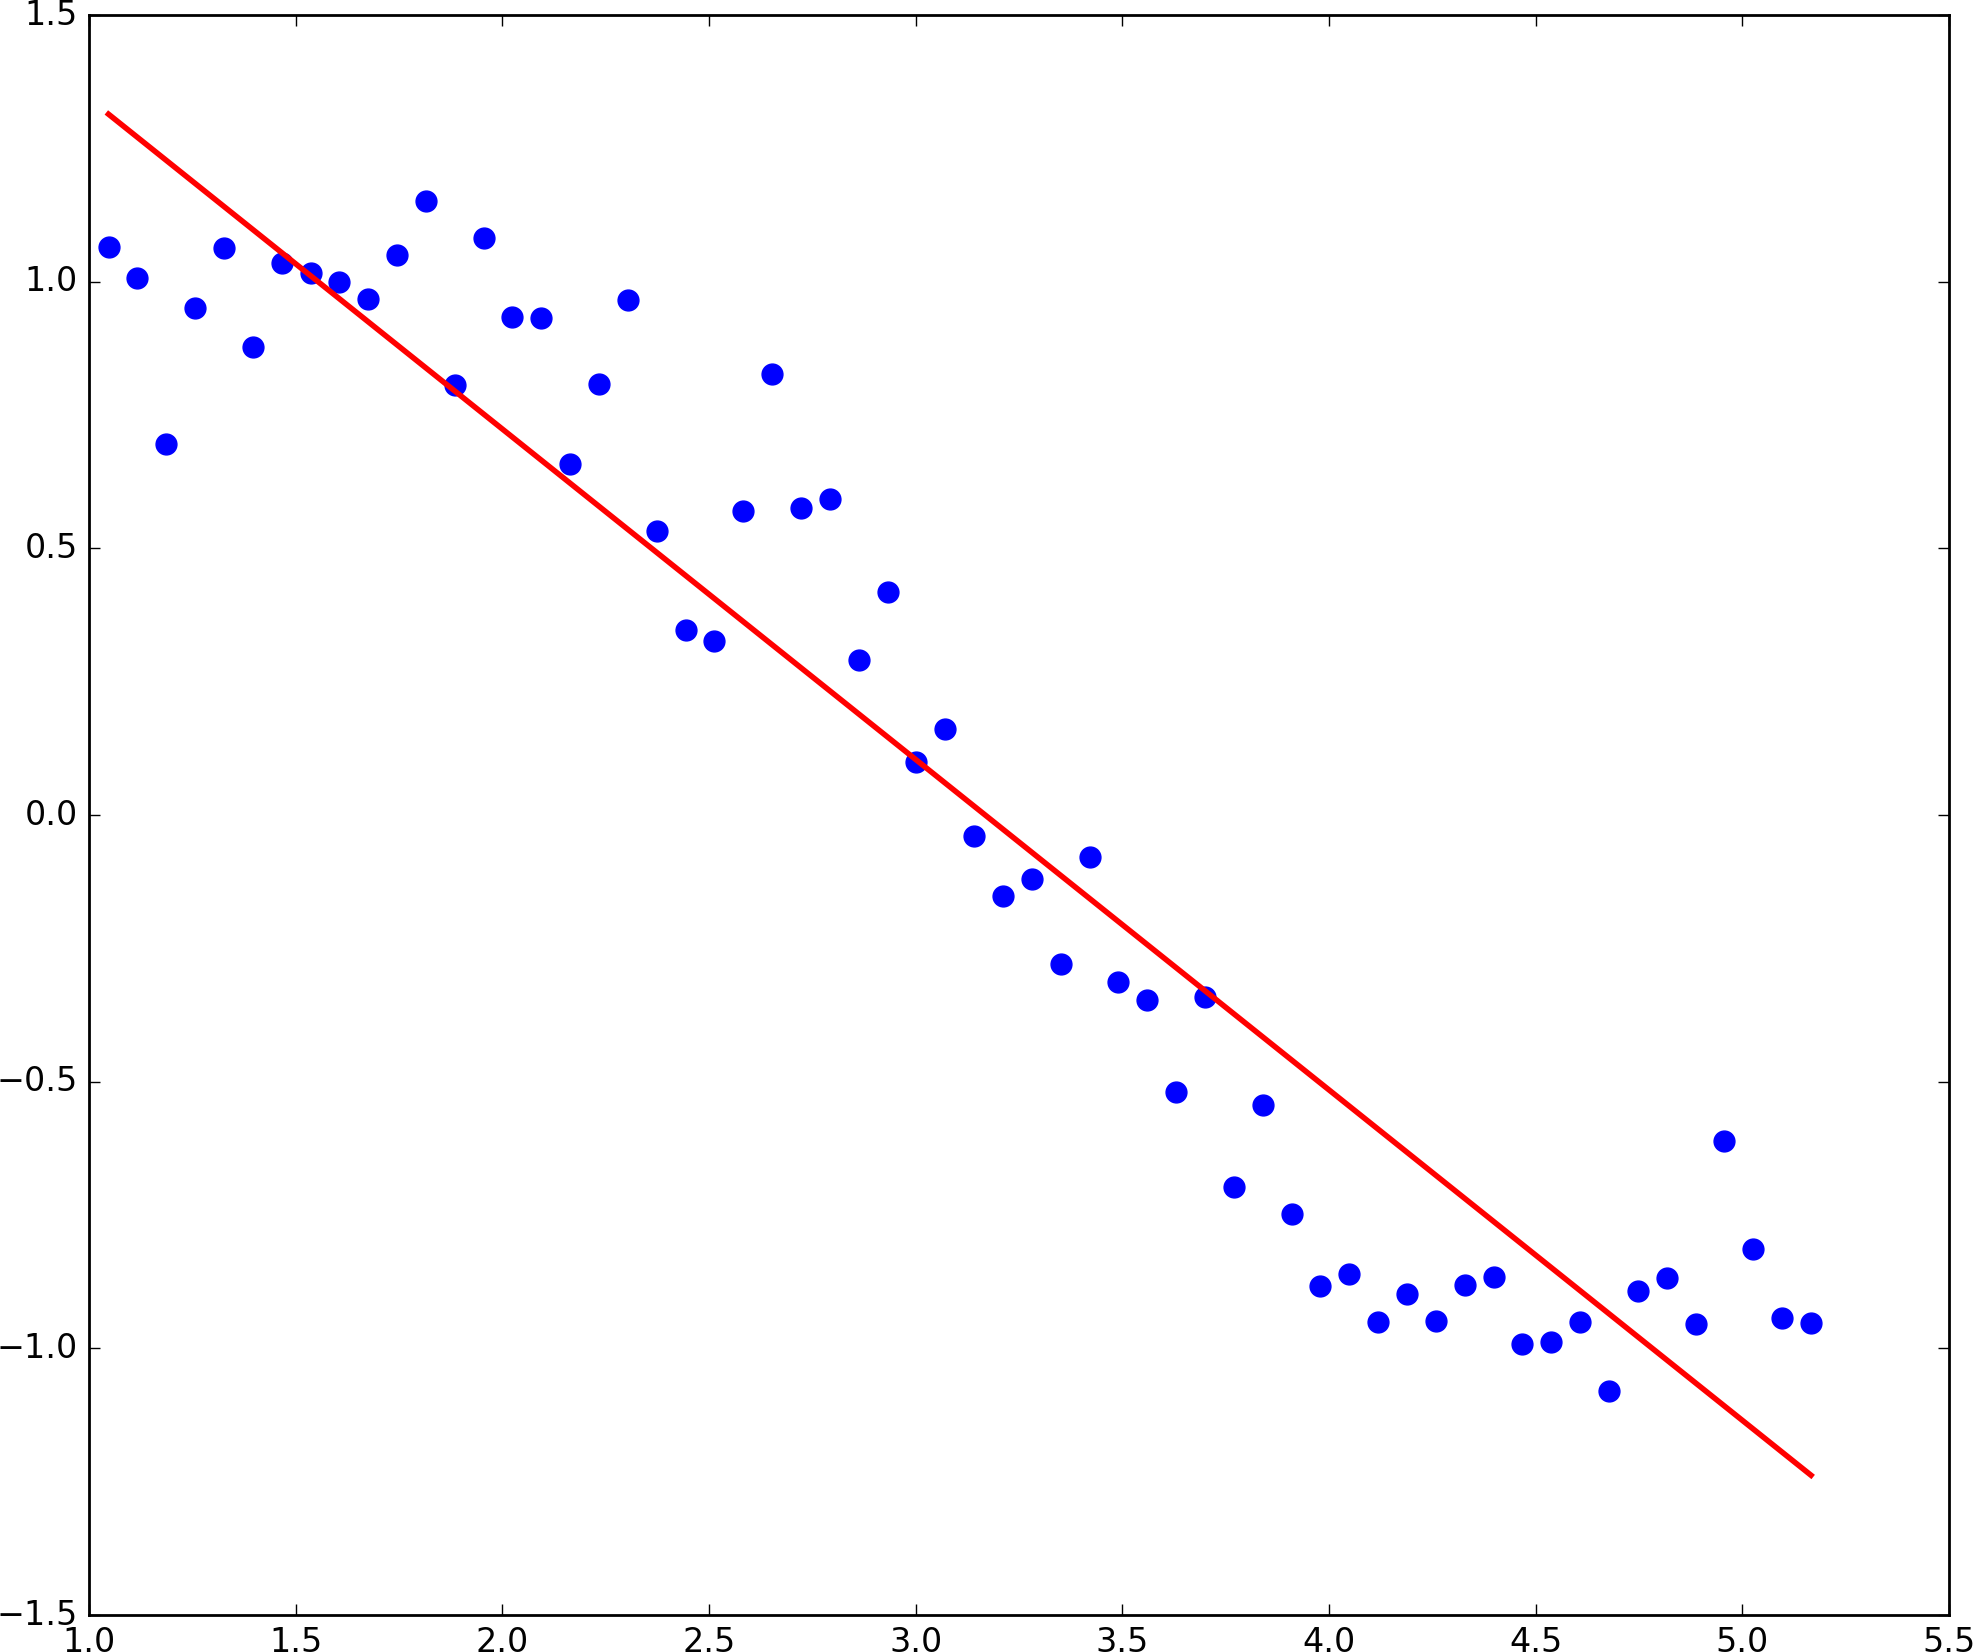
\includegraphics[width=0.99\textwidth]{./linreg_pow1.png}
\end{figure}
\vspace{-2em}
\begin{figure}
$p=9$
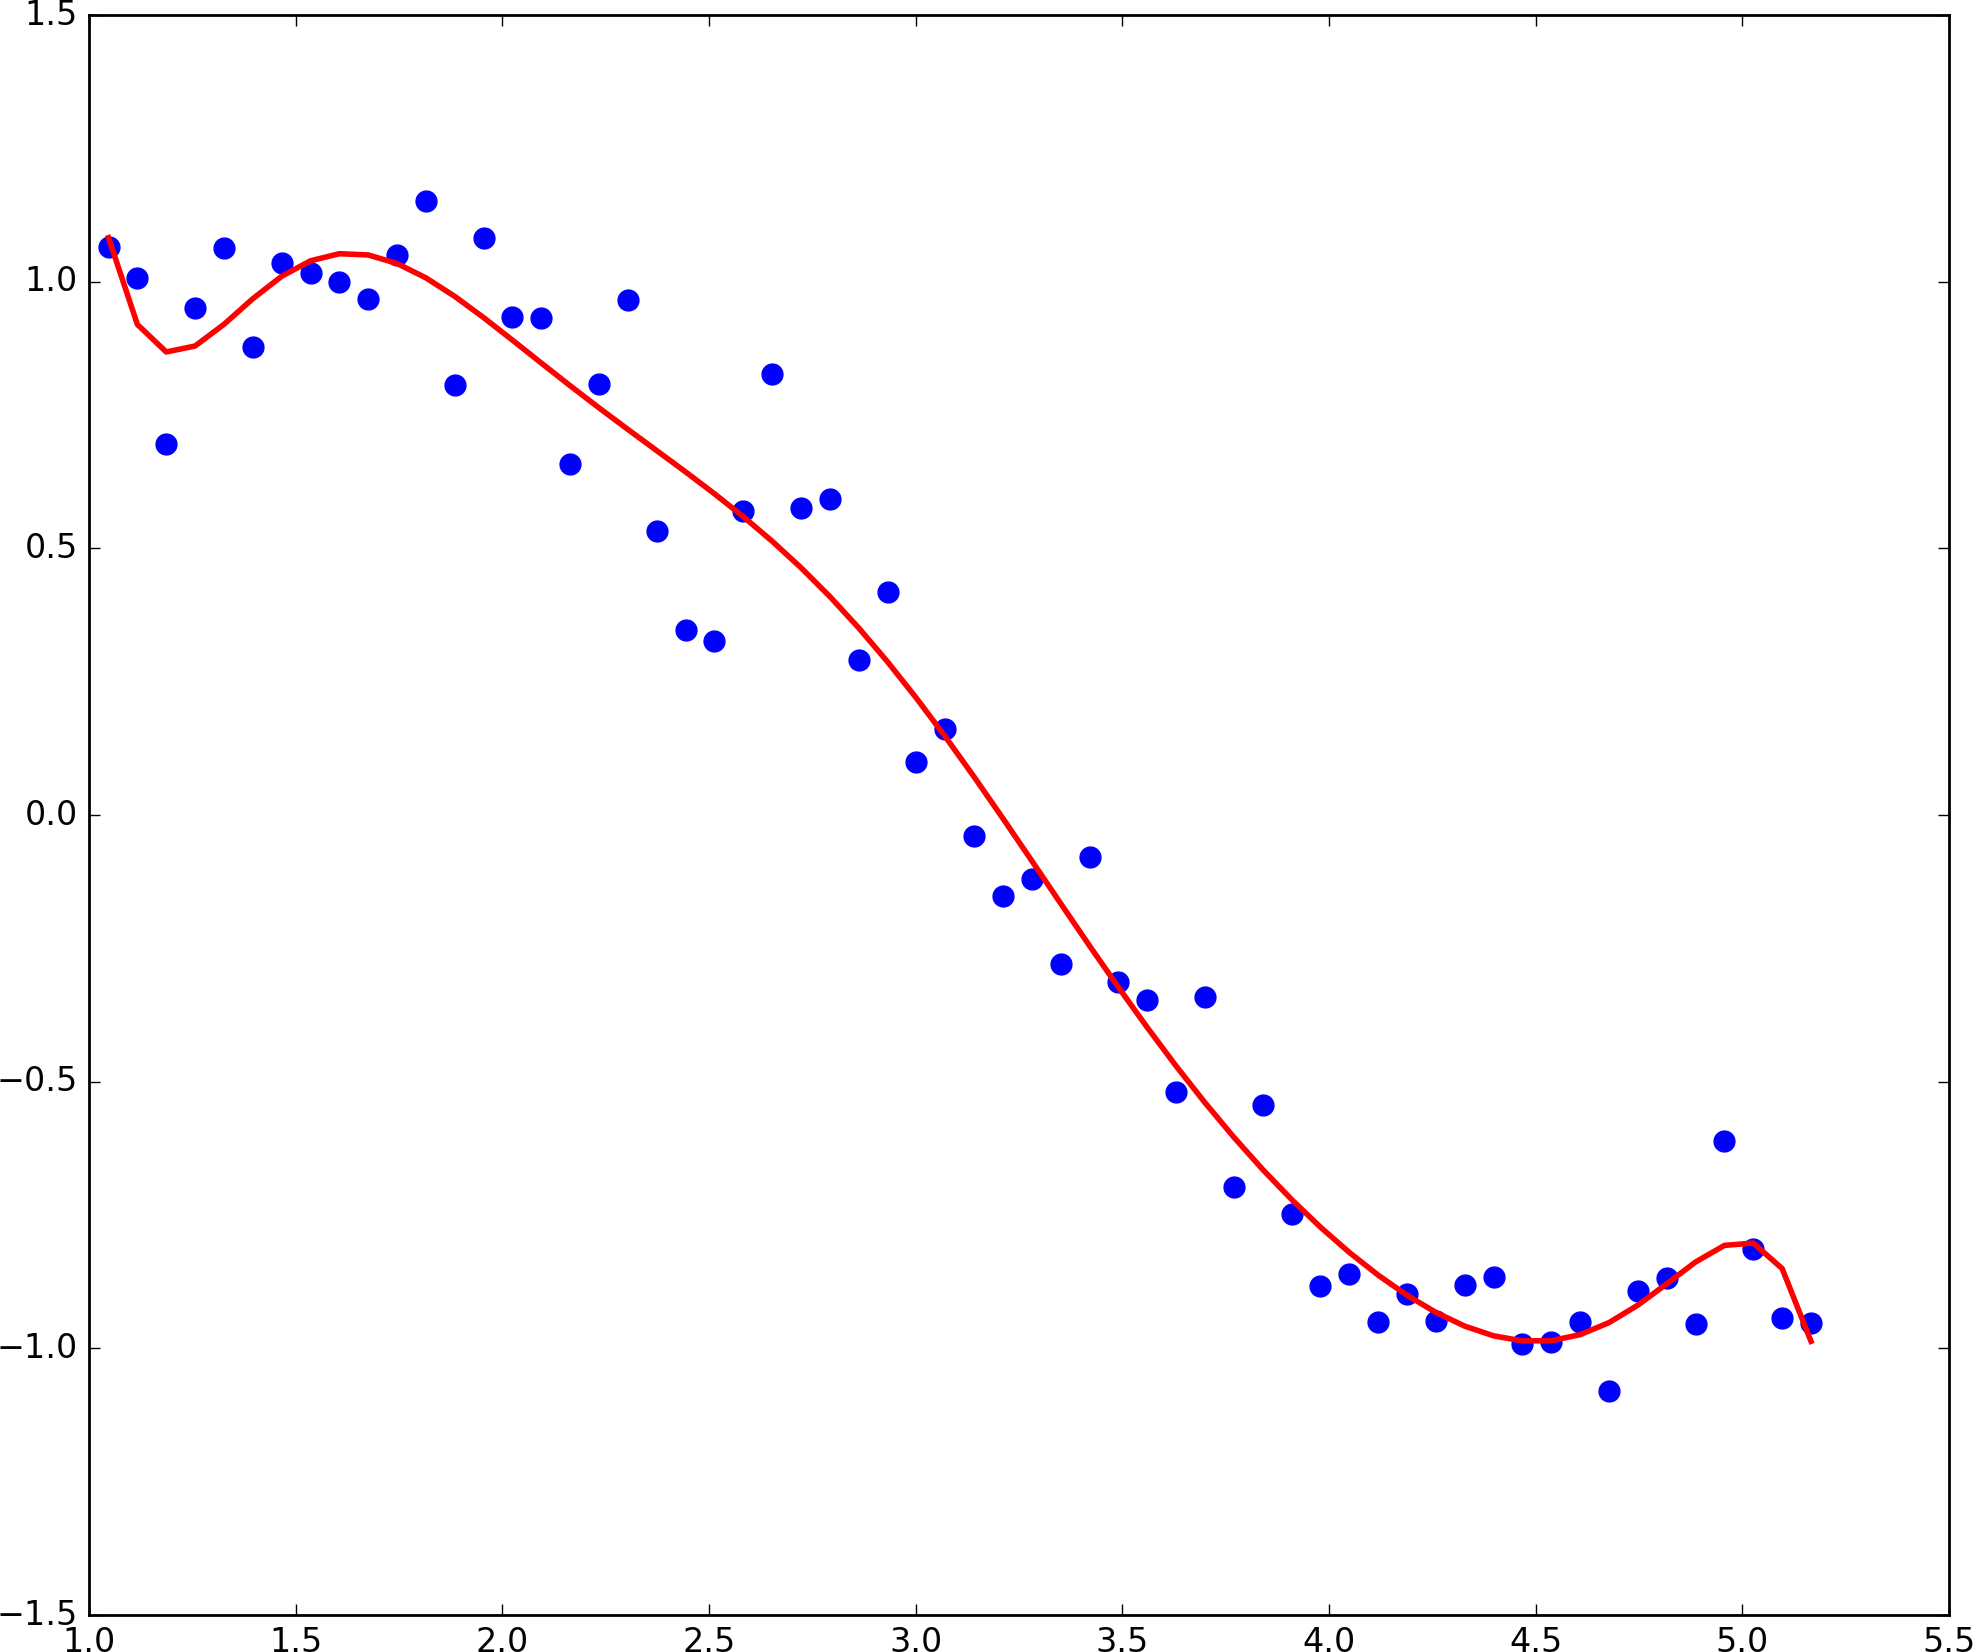
\includegraphics[width=0.99\textwidth]{./linreg_pow9.png}
\end{figure}
\column{.33\textwidth}
\vspace{-2em}
\begin{figure}
$p=3$
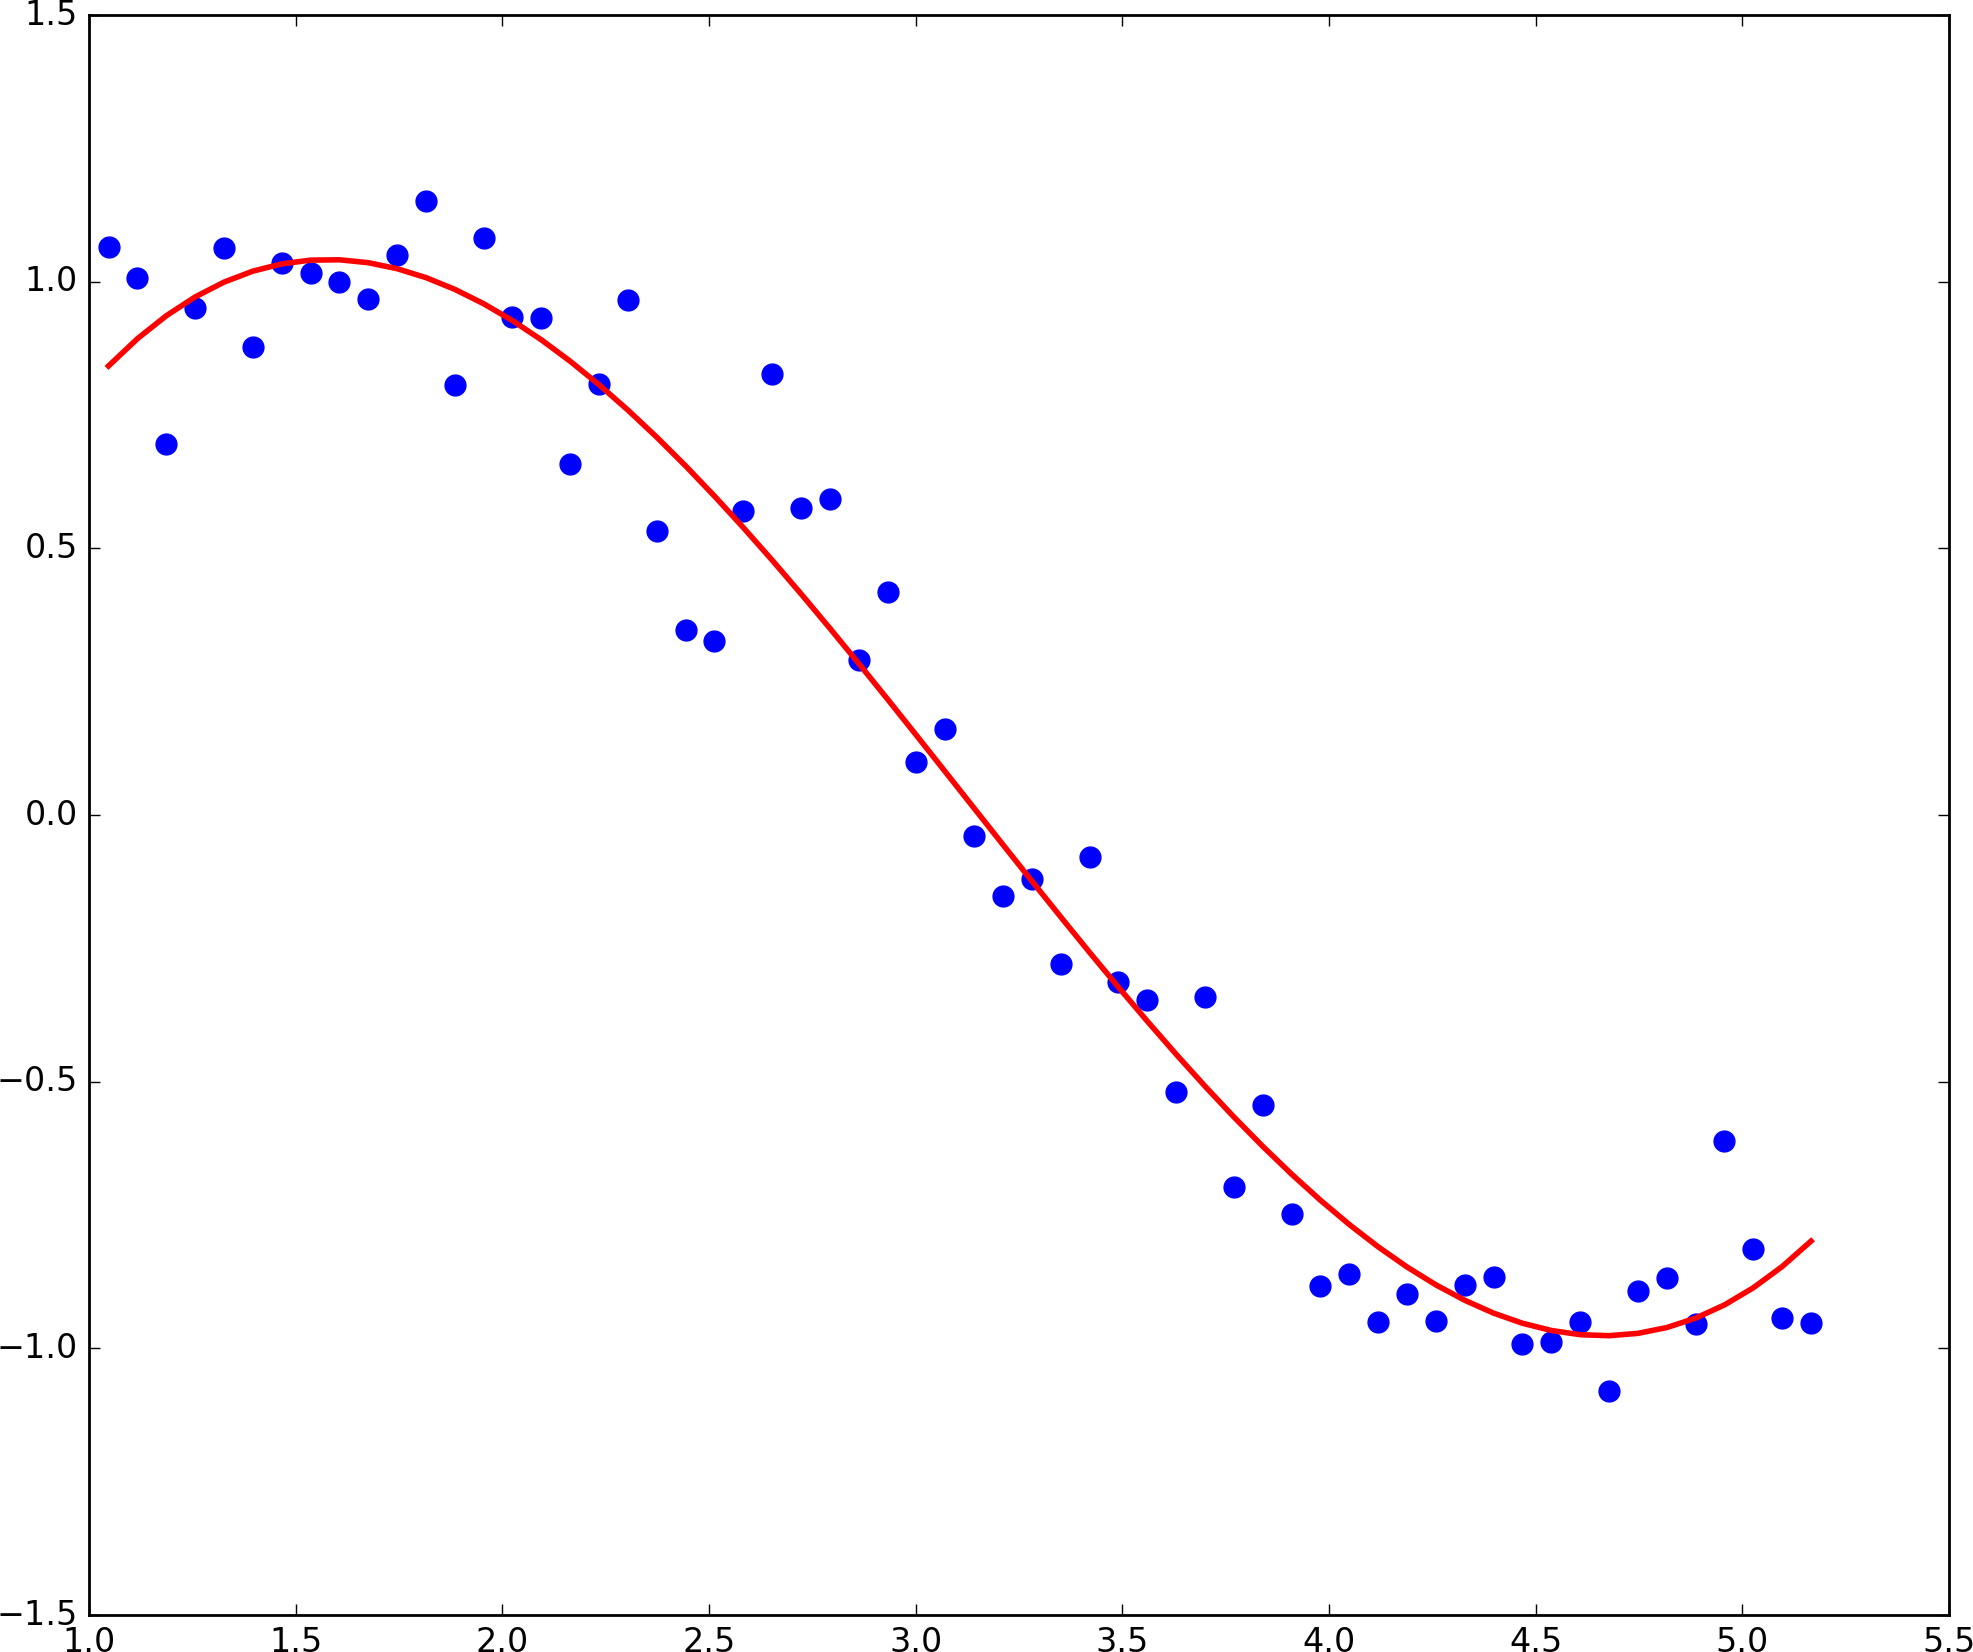
\includegraphics[width=0.99\textwidth]{./linreg_pow3.png}
\end{figure}
\vspace{-2em}
\begin{figure}
$p=12$
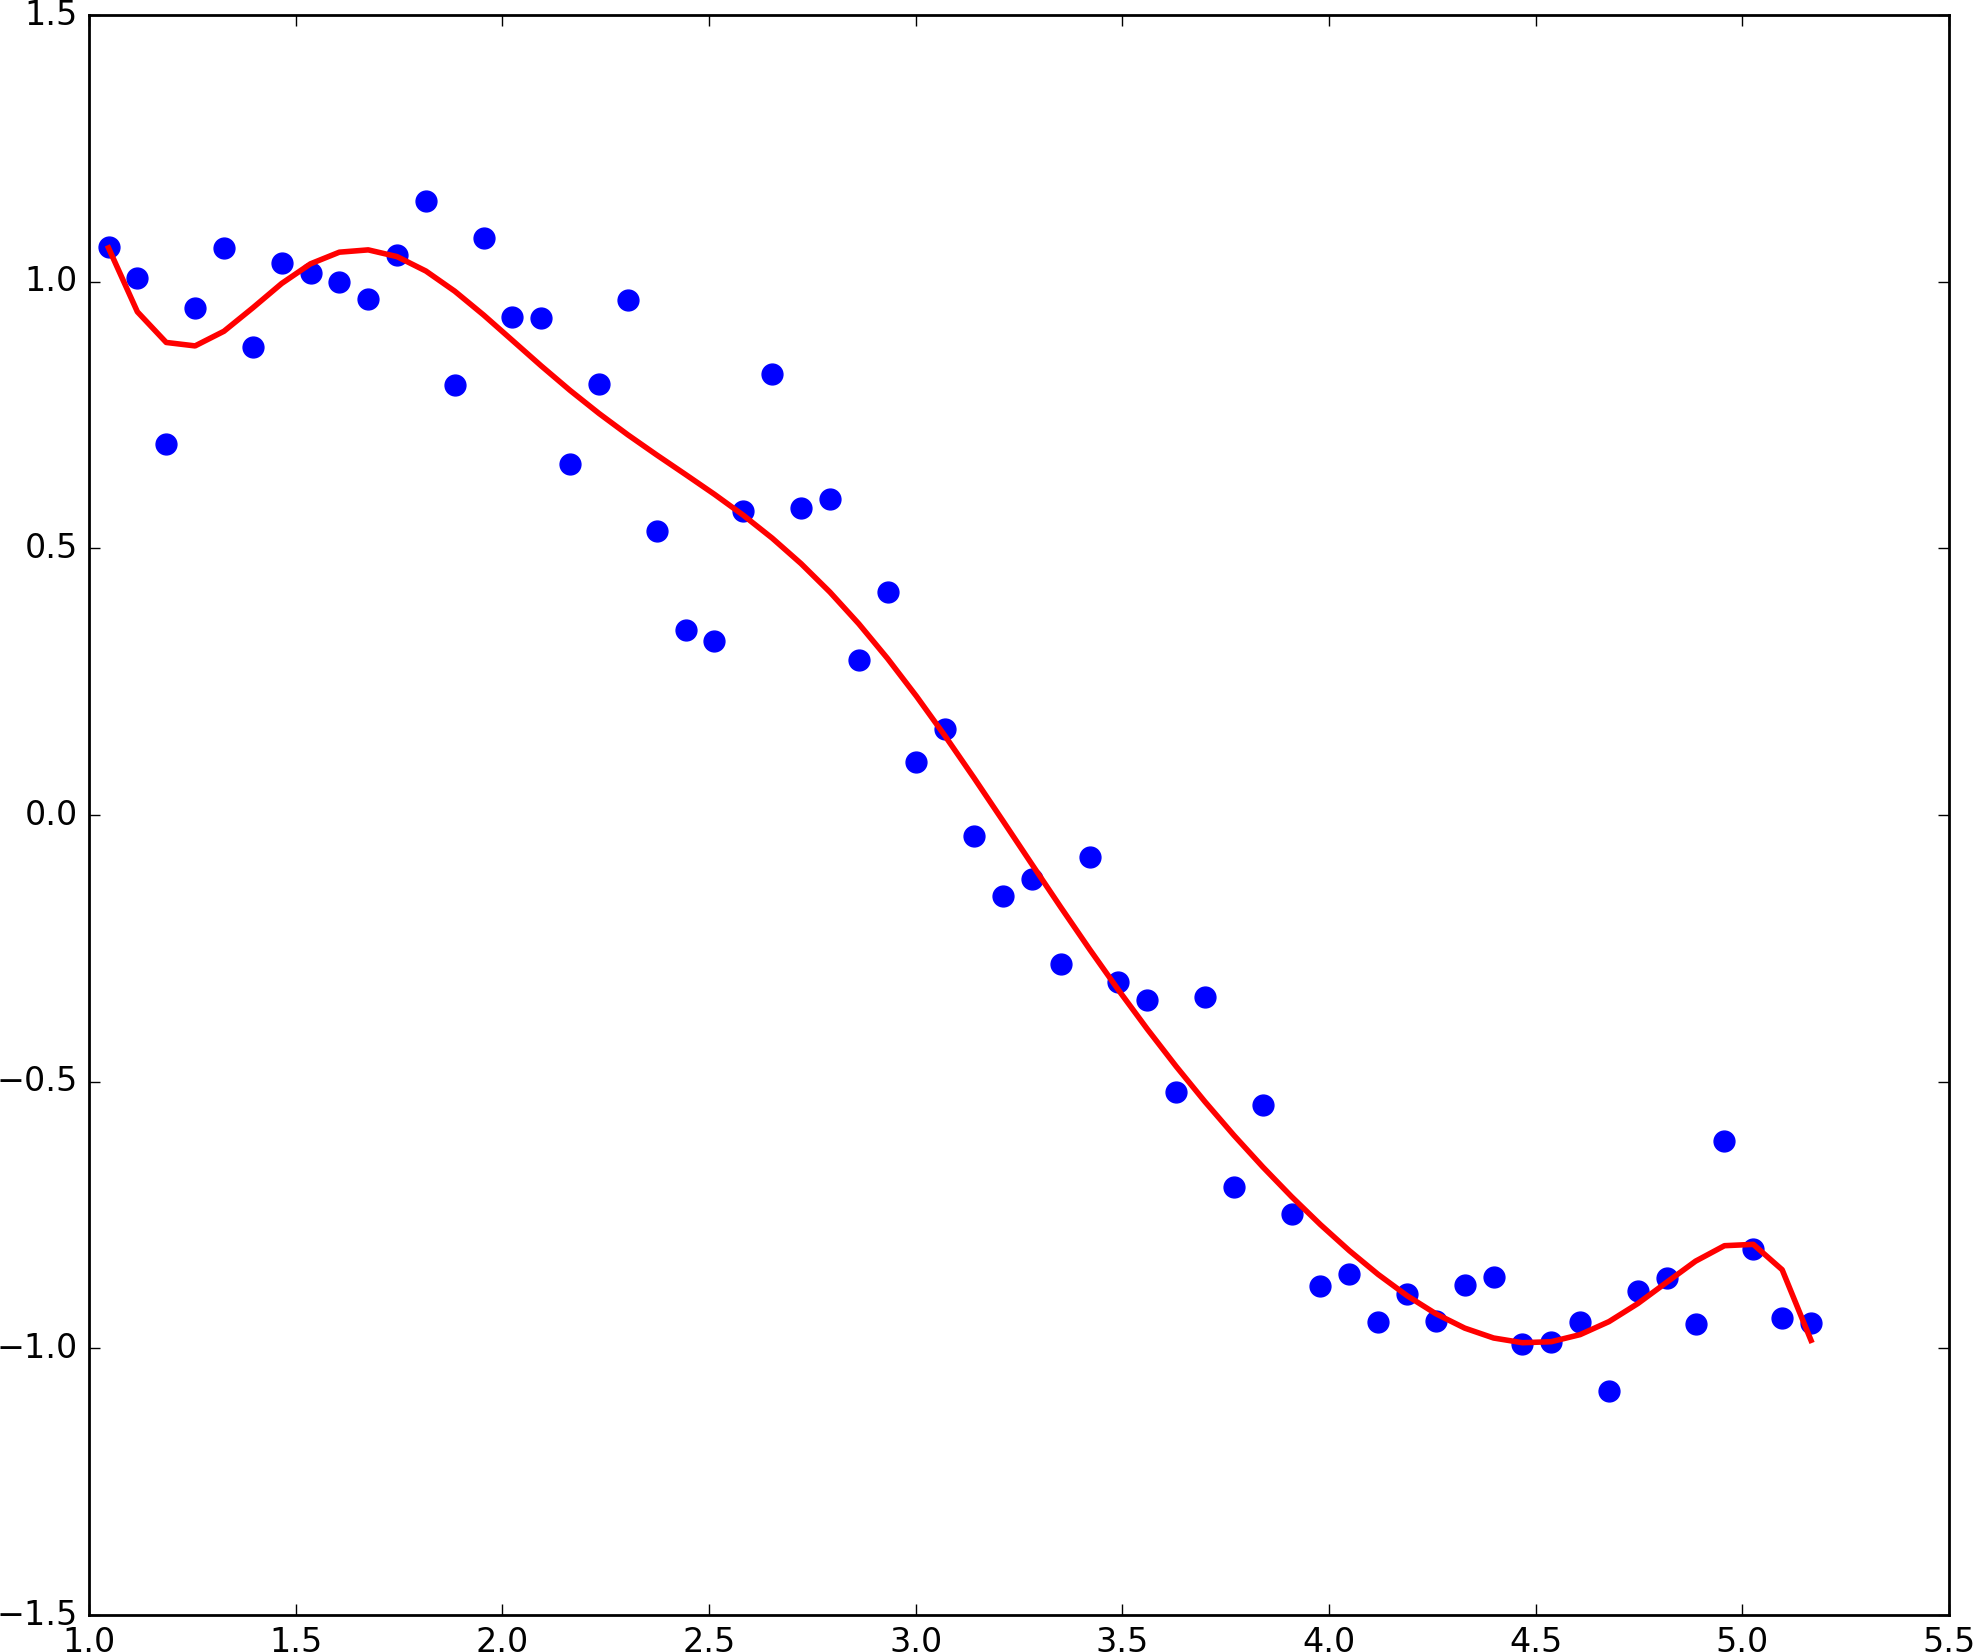
\includegraphics[width=0.99\textwidth]{./linreg_pow12.png}
\end{figure}
\column{.33\textwidth}
\vspace{-2em}
\begin{figure}
$p=4$
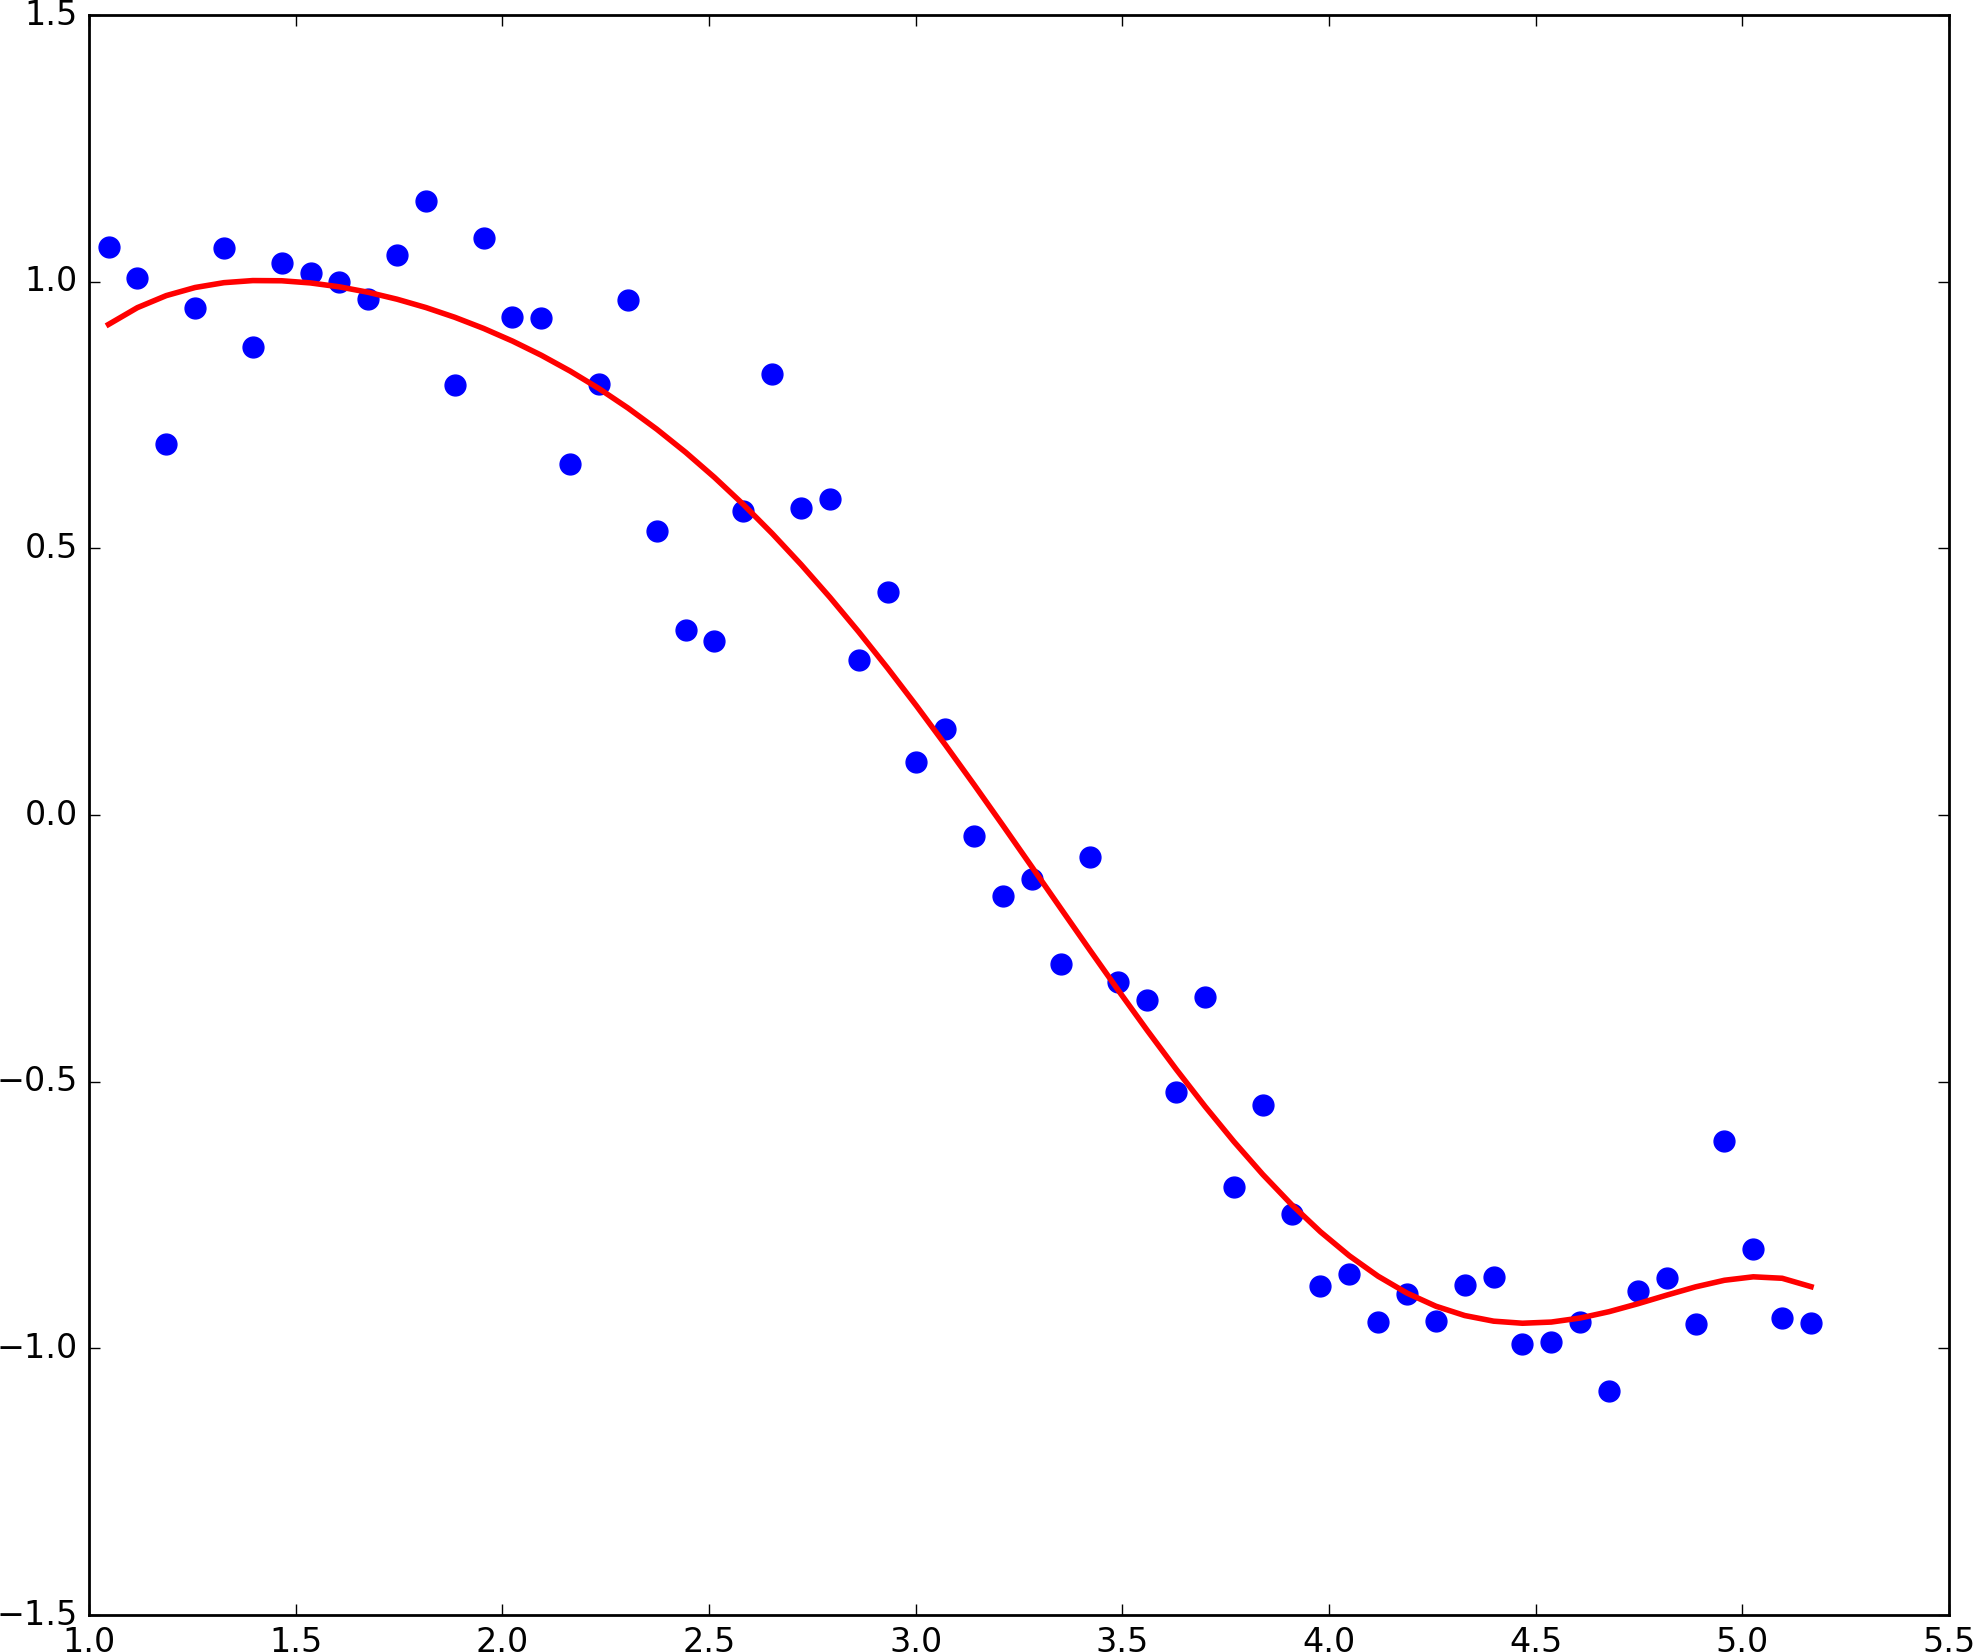
\includegraphics[width=0.99\textwidth]{./linreg_pow4.png}
\end{figure}
\vspace{-2em}
\begin{figure}
$p=15$
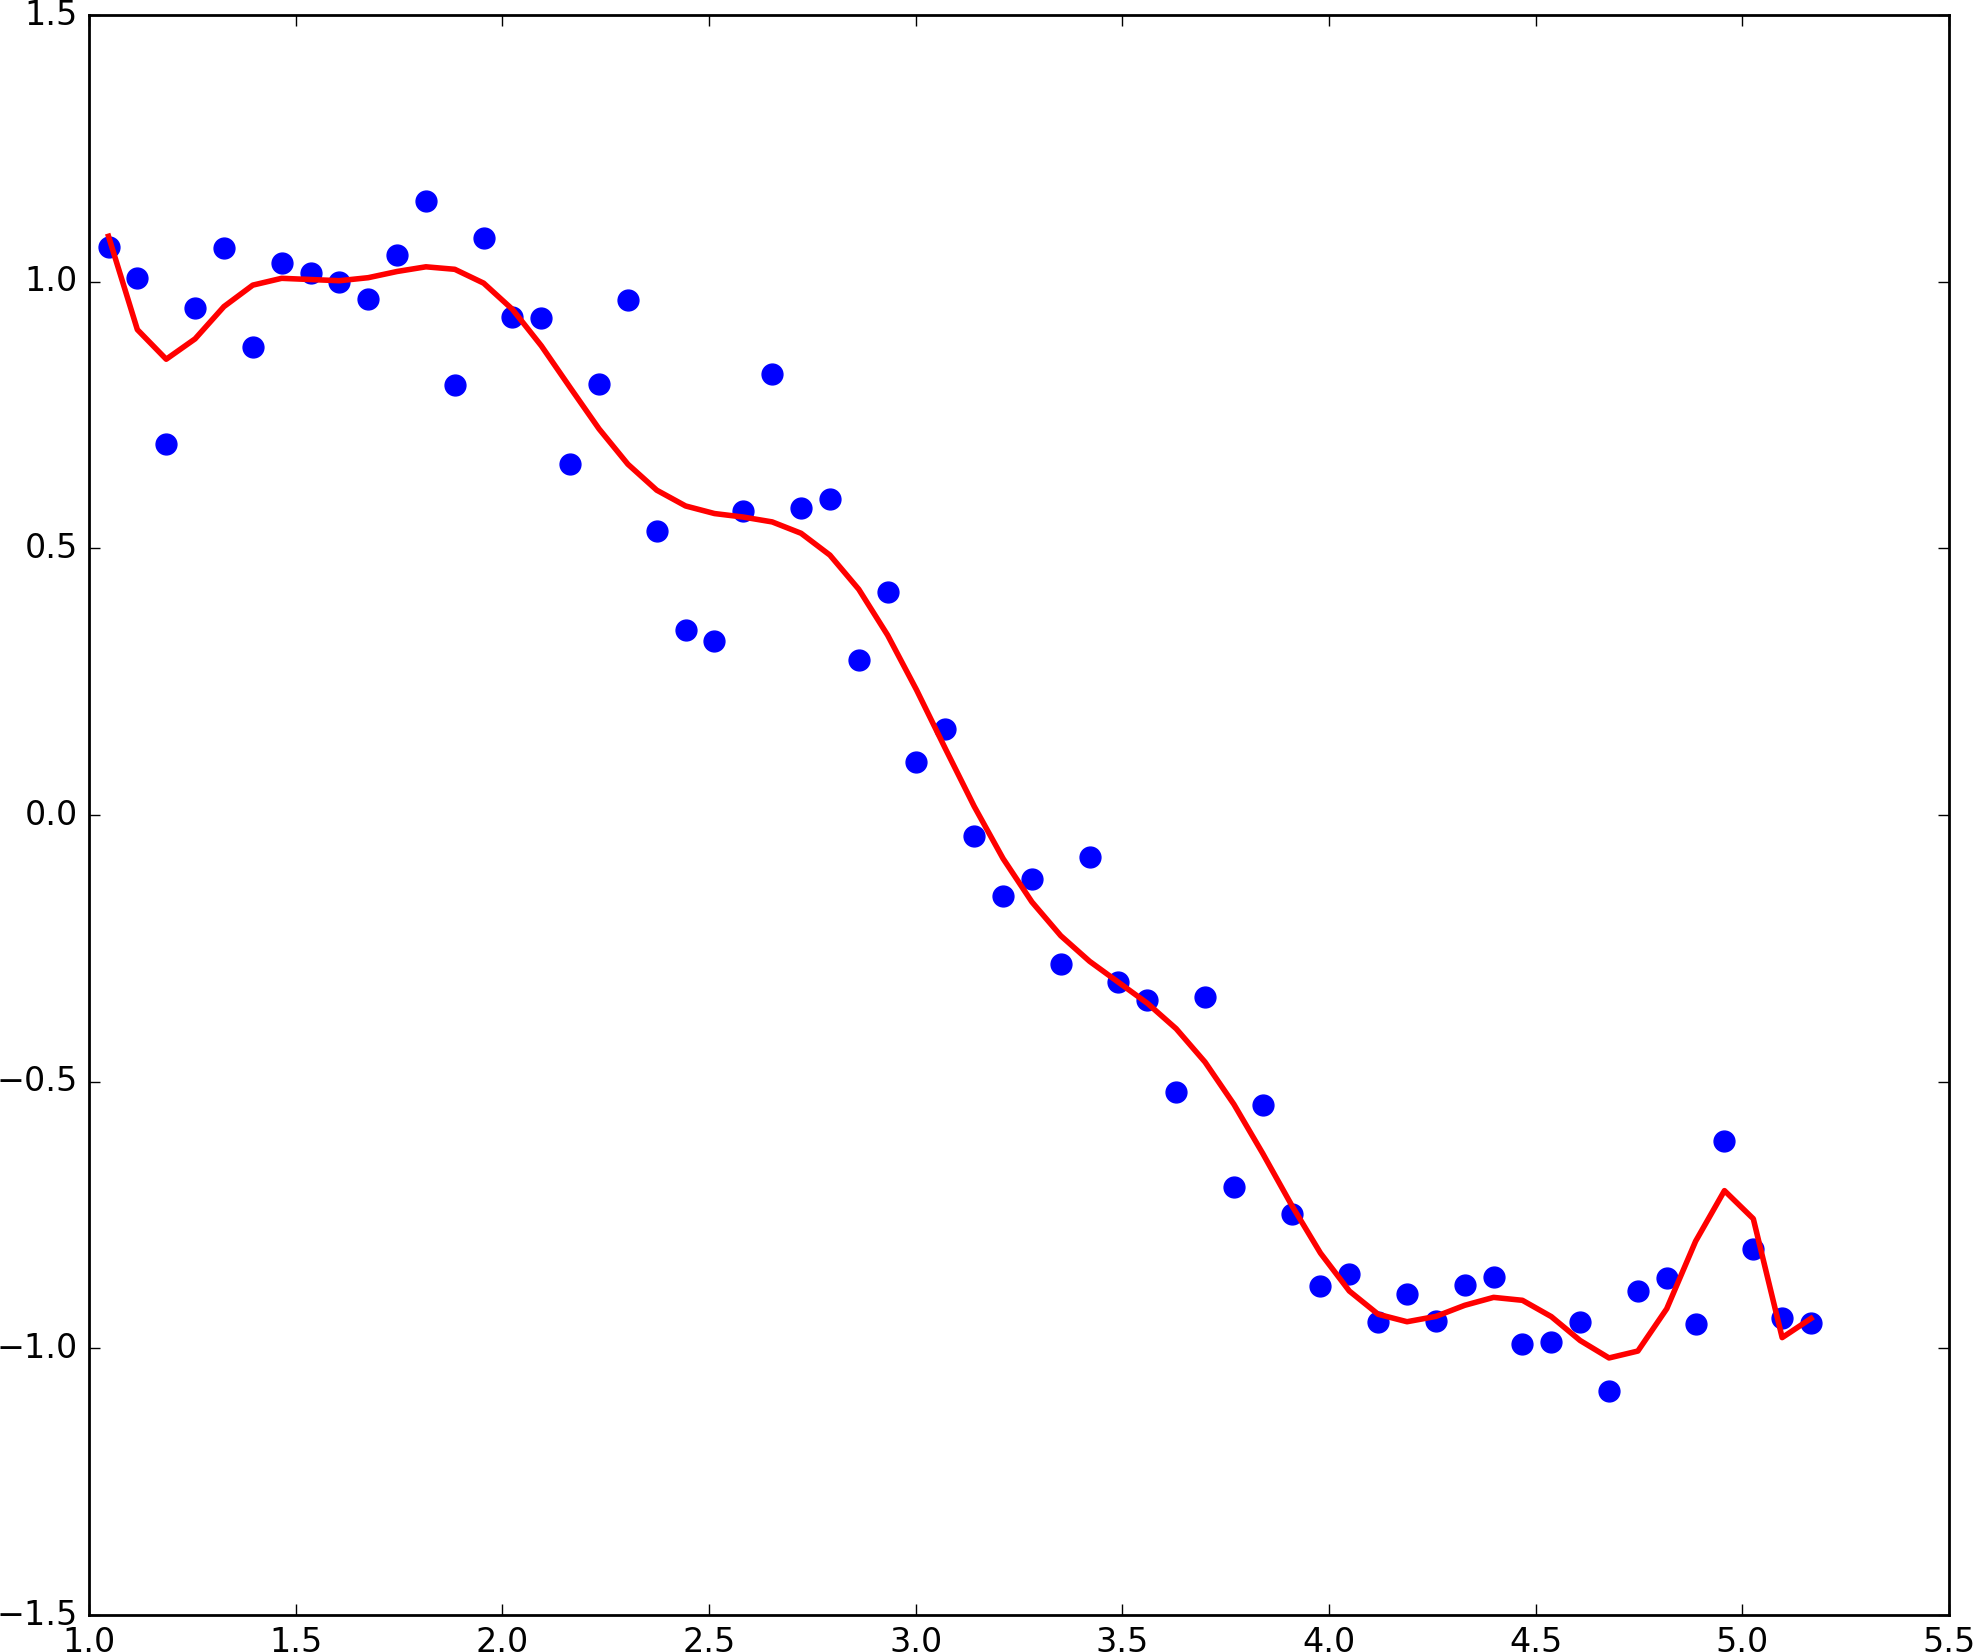
\includegraphics[width=0.99\textwidth]{./linreg_pow15.png}
\end{figure}
\end{columns}
\end{frame}


%%%%%%%%%%%%%%%%%%%%%
\begin{frame}
\frametitle{Overfitting}
\begin{block}{}
When there is to many paramaters to fit, the model can reproduce 
a random noise, it is called \alert{overfitting}
\end{block}
\pause
\begin{table}
\resizebox{\textwidth}{!}{%
\begin{tabular}{lllllllllll}
\toprule
{} &      rmse &      th\_0 &      th\_1 &      th\_2 &      th\_3 &      th\_4 &      th\_5 &      th\_6 &      th\_7 &      th\_8 \\
\midrule
max\_pow\_1  & +5.47e-02 & +1.96e+00 & -6.20e-01 &       NaN &       NaN &       NaN &       NaN &       NaN &       NaN &       NaN \\
max\_pow\_2  & +5.46e-02 & +1.91e+00 & -5.83e-01 & -5.96e-03 &       NaN &       NaN &       NaN &       NaN &       NaN &       NaN \\
max\_pow\_3  & +1.84e-02 & -1.08e+00 & +3.03e+00 & -1.29e+00 & +1.37e-01 &       NaN &       NaN &       NaN &       NaN &       NaN \\
max\_pow\_4  & +1.80e-02 & -2.66e-01 & +1.69e+00 & -5.32e-01 & -3.57e-02 & +1.39e-02 &       NaN &       NaN &       NaN &       NaN \\
max\_pow\_5  & +1.70e-02 & +2.99e+00 & -5.12e+00 & +4.72e+00 & -1.93e+00 & +3.35e-01 & -2.07e-02 &       NaN &       NaN &       NaN \\
max\_pow\_6  & +1.65e-02 & -2.80e+00 & +9.52e+00 & -9.71e+00 & +5.23e+00 & -1.55e+00 & +2.33e-01 & -1.36e-02 &       NaN &       NaN \\
max\_pow\_7  & +1.55e-02 & +1.93e+01 & -5.60e+01 & +6.90e+01 & -4.46e+01 & +1.65e+01 & -3.53e+00 & +4.05e-01 & -1.92e-02 &       NaN \\
max\_pow\_8  & +1.53e-02 & +4.32e+01 & -1.37e+02 & +1.84e+02 & -1.33e+02 & +5.77e+01 & -1.53e+01 & +2.42e+00 & -2.10e-01 & +7.68e-03 \\
max\_pow\_9  & +1.46e-02 & +1.68e+02 & -6.15e+02 & +9.63e+02 & -8.46e+02 & +4.61e+02 & -1.62e+02 & +3.68e+01 & -5.22e+00 & +4.22e-01 \\
max\_pow\_10 & +1.46e-02 & +1.38e+02 & -4.86e+02 & +7.26e+02 & -5.96e+02 & +2.93e+02 & -8.75e+01 & +1.45e+01 & -8.06e-01 & -1.38e-01 \\
max\_pow\_11 & +1.45e-02 & -7.49e+01 & +5.12e+02 & -1.33e+03 & +1.87e+03 & -1.61e+03 & +9.14e+02 & -3.50e+02 & +9.14e+01 & -1.61e+01 \\
max\_pow\_12 & +1.45e-02 & -3.39e+02 & +1.87e+03 & -4.42e+03 & +6.01e+03 & -5.25e+03 & +3.12e+03 & -1.30e+03 & +3.84e+02 & -8.03e+01 \\
max\_pow\_13 & +1.43e-02 & +3.20e+03 & -1.78e+04 & +4.46e+04 & -6.66e+04 & +6.61e+04 & -4.61e+04 & +2.32e+04 & -8.55e+03 & +2.30e+03 \\
max\_pow\_14 & +1.31e-02 & +2.38e+04 & -1.41e+05 & +3.79e+05 & -6.10e+05 & +6.57e+05 & -5.03e+05 & +2.82e+05 & -1.17e+05 & +3.66e+04 \\
max\_pow\_15 & +1.17e-02 & -3.62e+04 & +2.44e+05 & -7.46e+05 & +1.38e+06 & -1.71e+06 & +1.53e+06 & -1.00e+06 & +4.98e+05 & -1.88e+05 \\
\bottomrule
\end{tabular}
}
\end{table}
\end{frame}


%%%%%%%%%%%%%%%%%%%%%%%
\begin{frame}
\frametitle{High parameters values}
\begin{figure}
Value of the parameters $|\theta_1|$ with respect with the degree of the polynomial
regression\\
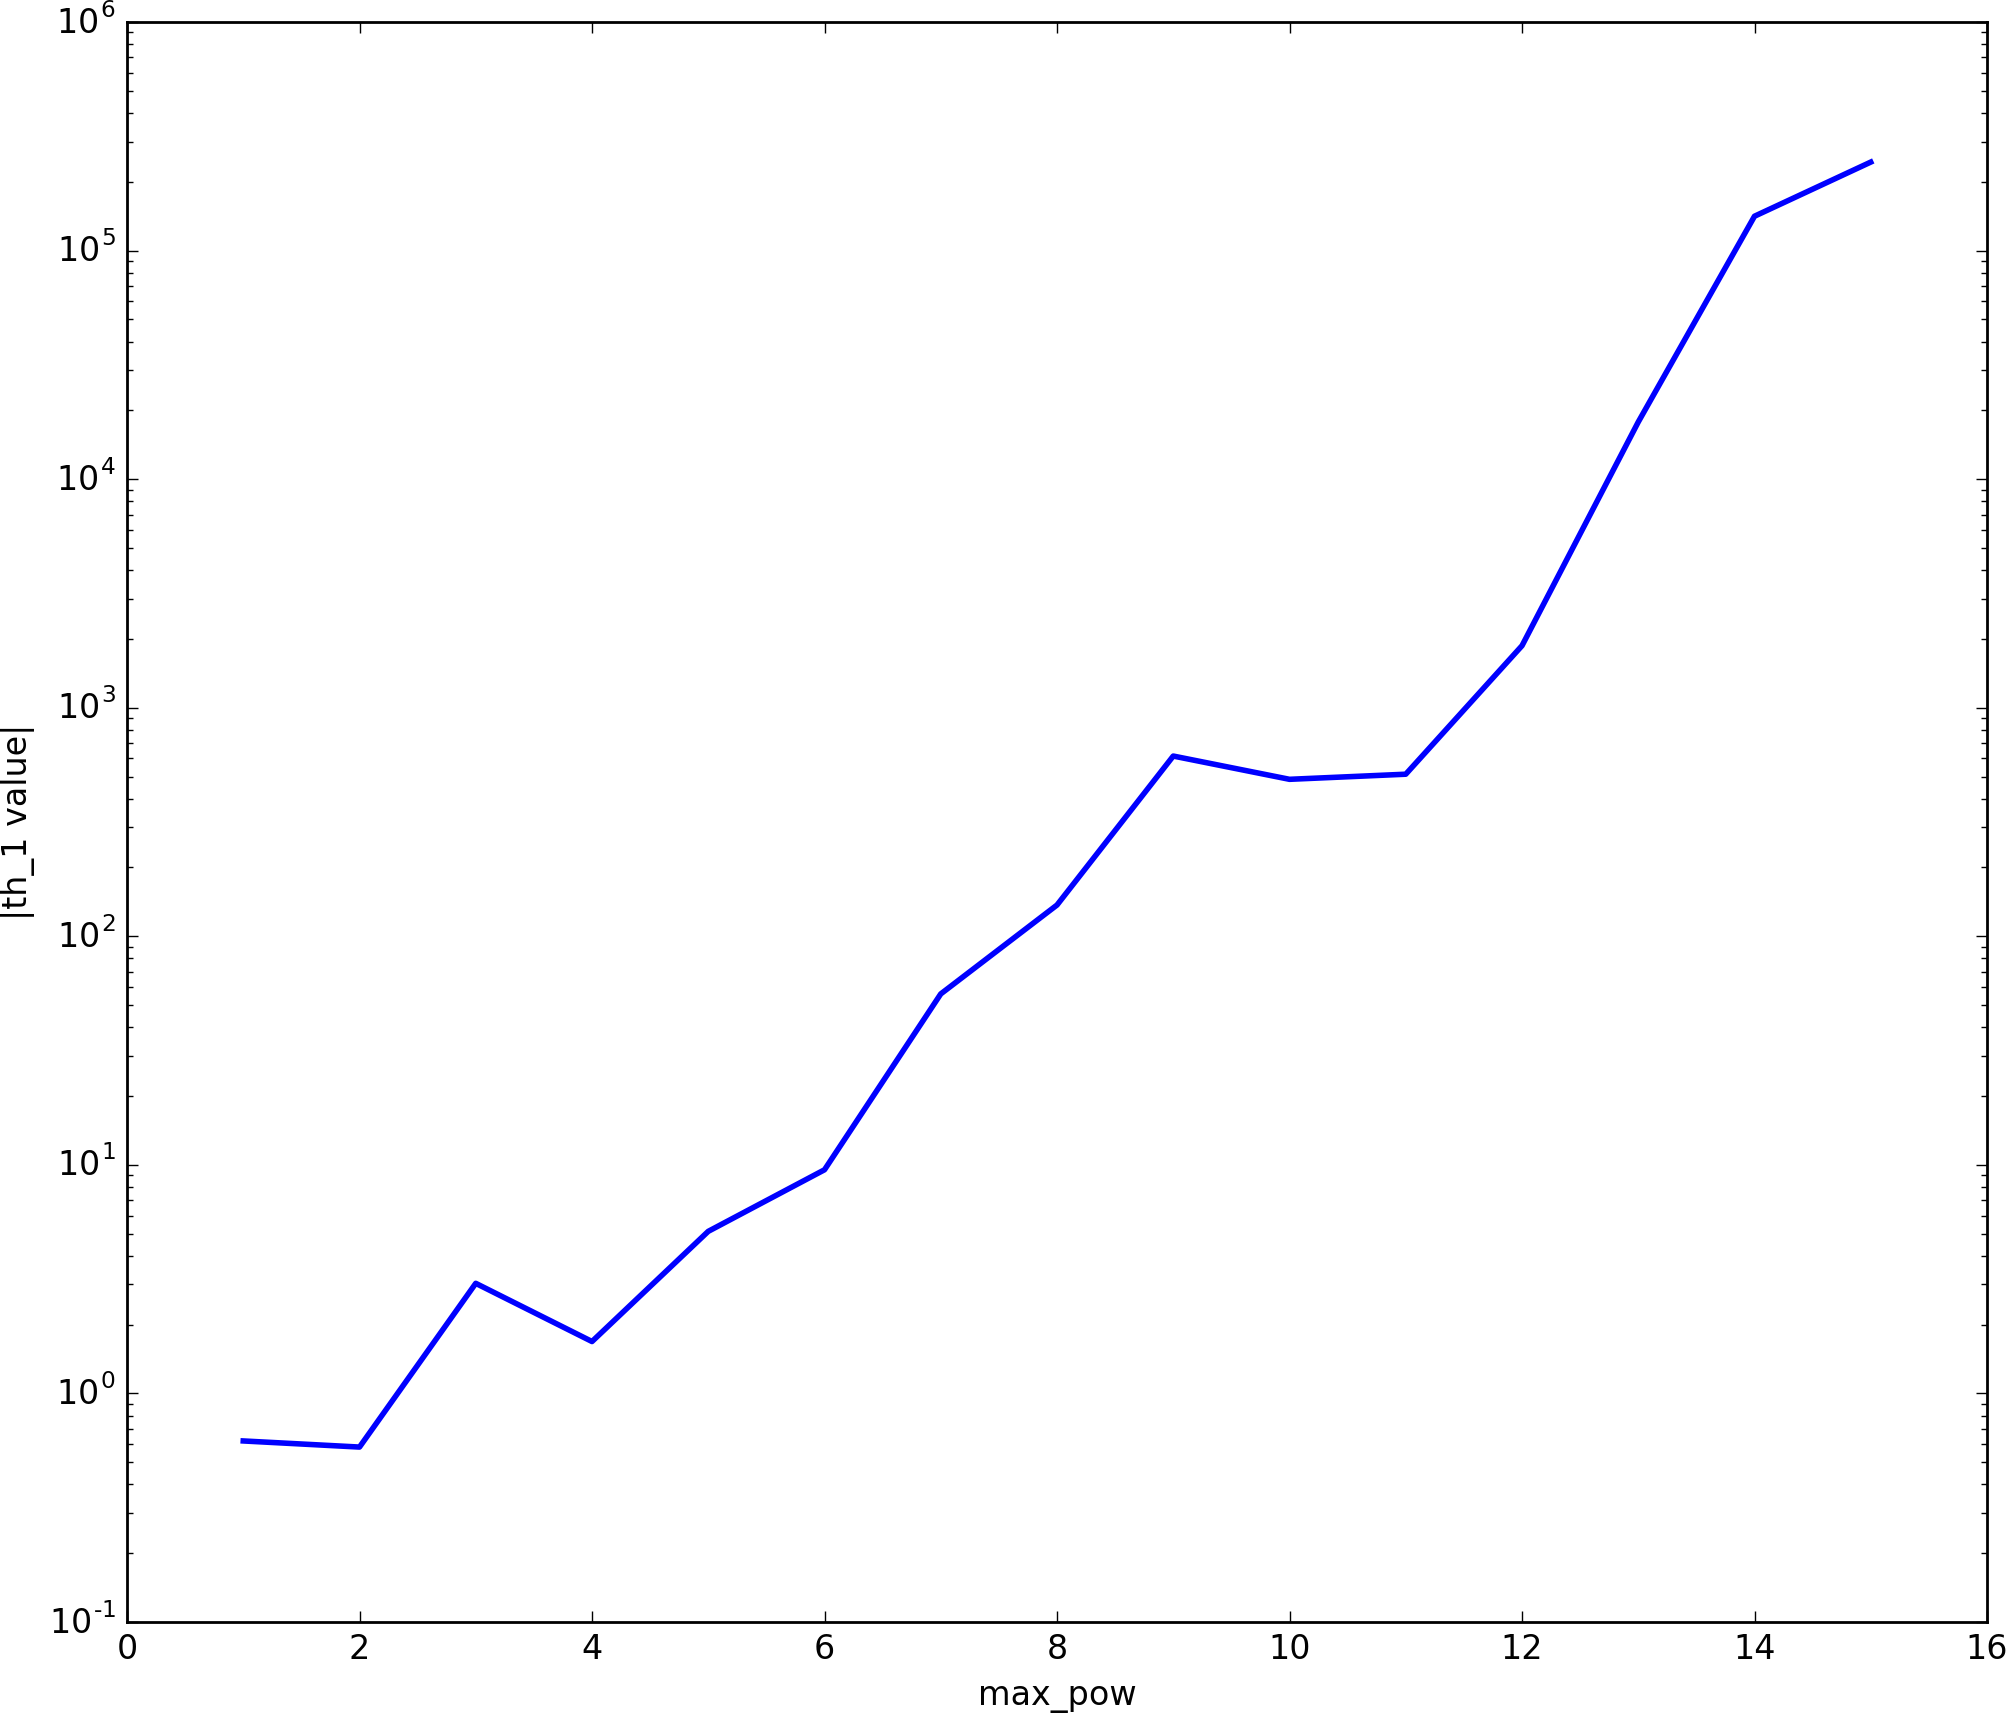
\includegraphics[height=0.75\textheight]{./coefs_th1.png}
\end{figure}

\end{frame}

%%%%%%%%%%%%%%%%%%%%%
\begin{frame}
\frametitle{Regularization}
\begin{block}{The idea}
The idea of regularization is to perform a regression minimizing a cost function
that includes a term to penalize "big" values for the parameters:
$$
J(\bm{\theta}) = \frac{1}{n} \sum (y_i - h_{\bm{\theta}}(x_i))^2 + \alpha P(\bm{\theta})
$$
\end{block}
\pause
We consider two penalty terms:
\begin{itemize}[<+->]
\item \alert{Ridge Regularization (L2):} $P(\bm{\theta}) = \sum_{i=0}^p \theta_i^2$
\item \alert{Lasso Regularization (L1):} $P(\bm{\theta}) = \sum_{i=0}^p |\theta_i|$
\item Elastic Net combines both regularization
\end{itemize}

\end{frame}

%%%%%%%%%%%%%%%%%%%%
\begin{frame}
\frametitle{Ridge regression (L2)}
\begin{block}{}
Ridge regression is a linear regression with a Ridge regularization:
$$
J(\bm{\theta}) = \frac{1}{n} \sum (y_i - h_{\bm{\theta}}(x_i))^2 + \alpha \sum_{i=0}^p \theta_i^2
$$
\end{block}
\end{frame}

%%%%%%%%%%%%%%%%%%%%
\begin{frame}
\frametitle{Results for $p=15$ and varying $\alpha$}
\begin{columns}
\column{.33\textwidth}
\vspace{-2em}
\begin{figure}
$\alpha=0$
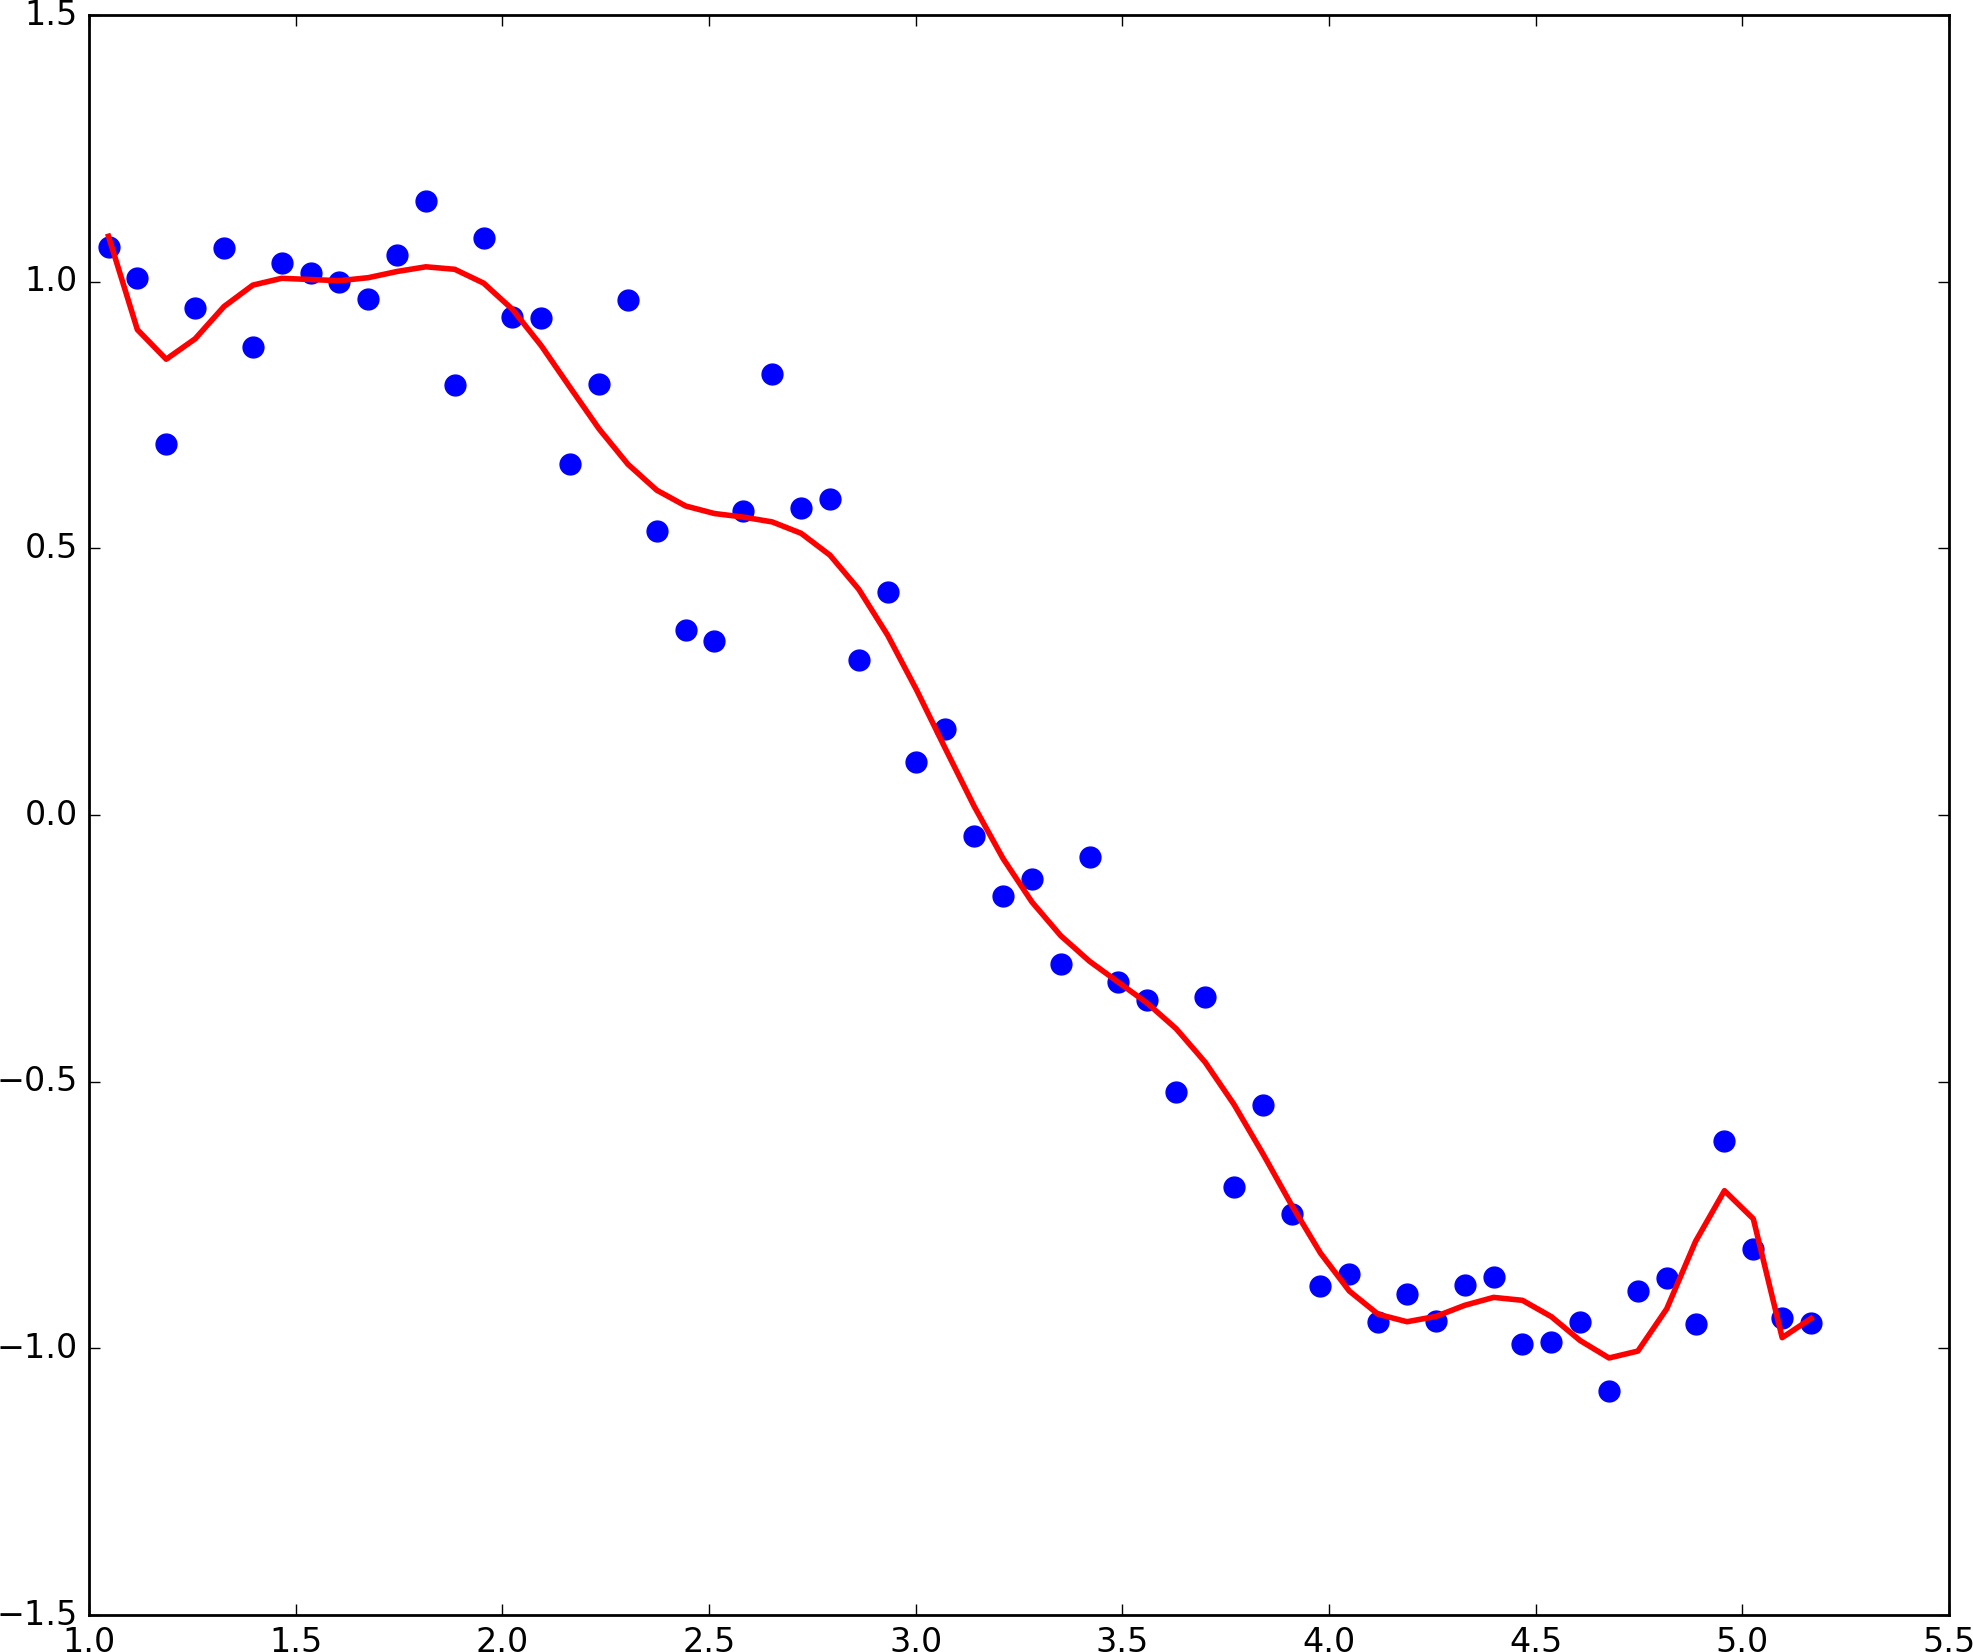
\includegraphics[width=0.99\textwidth]{./ridge_alpha0.png}
\end{figure}
\vspace{-2em}
\begin{figure}
$\alpha=1e-3$
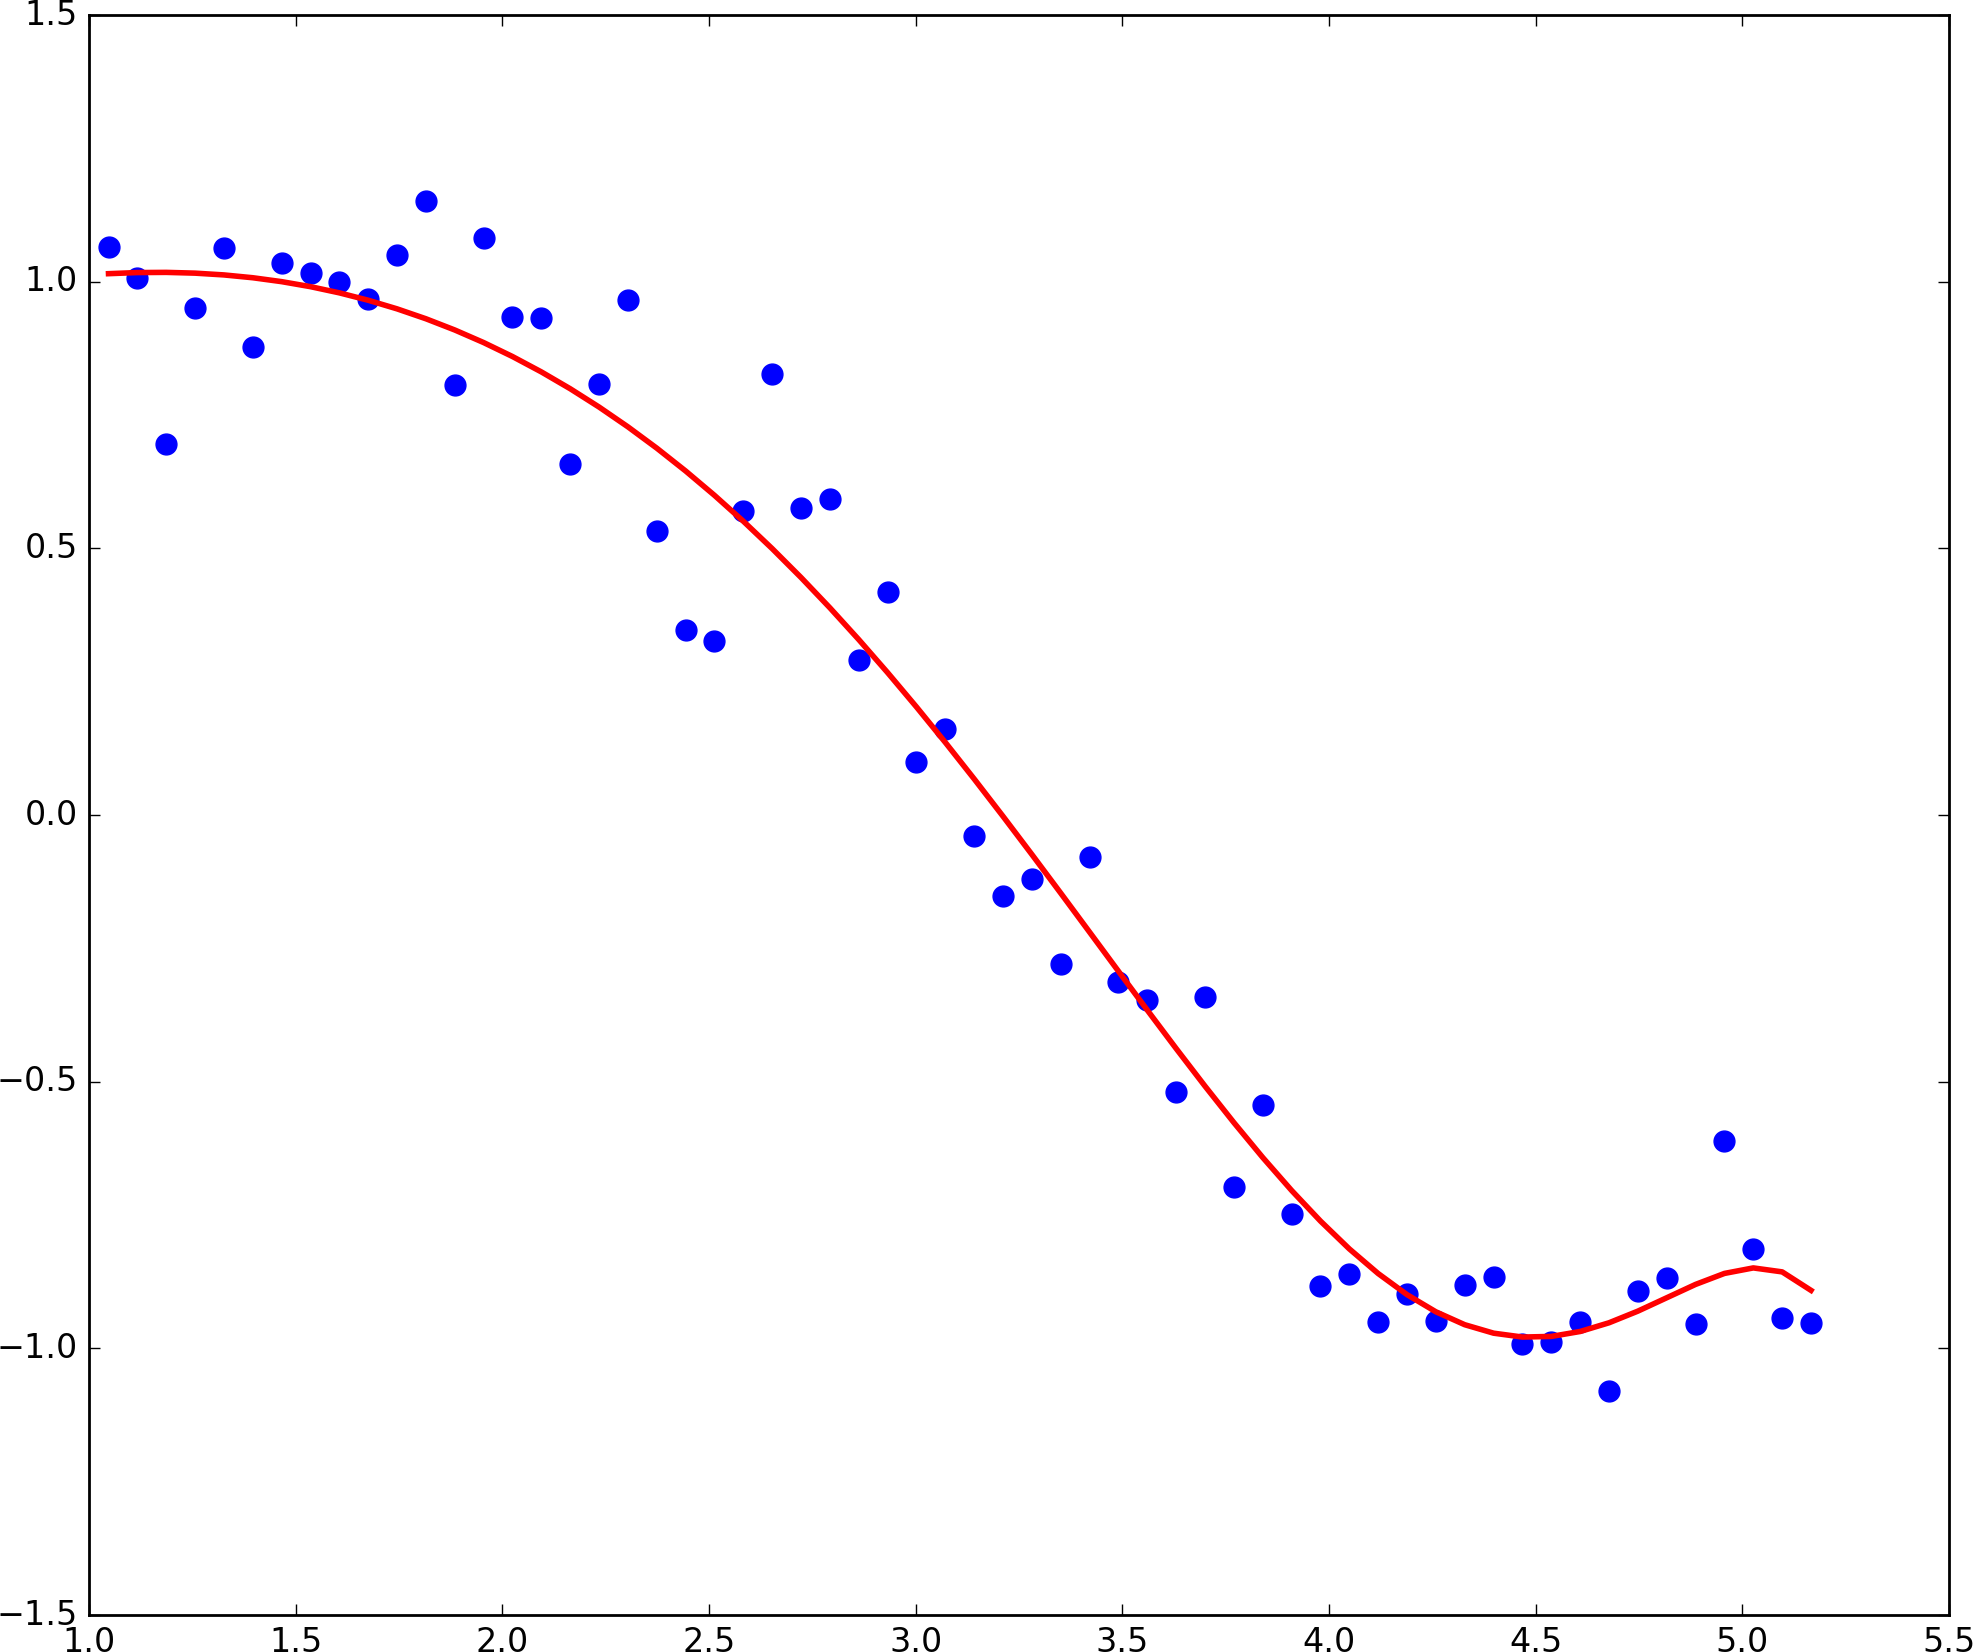
\includegraphics[width=0.99\textwidth]{./ridge_alpha1e-3.png}
\end{figure}
\column{.33\textwidth}
\vspace{-2em}
\begin{figure}
$\alpha=1e-15$
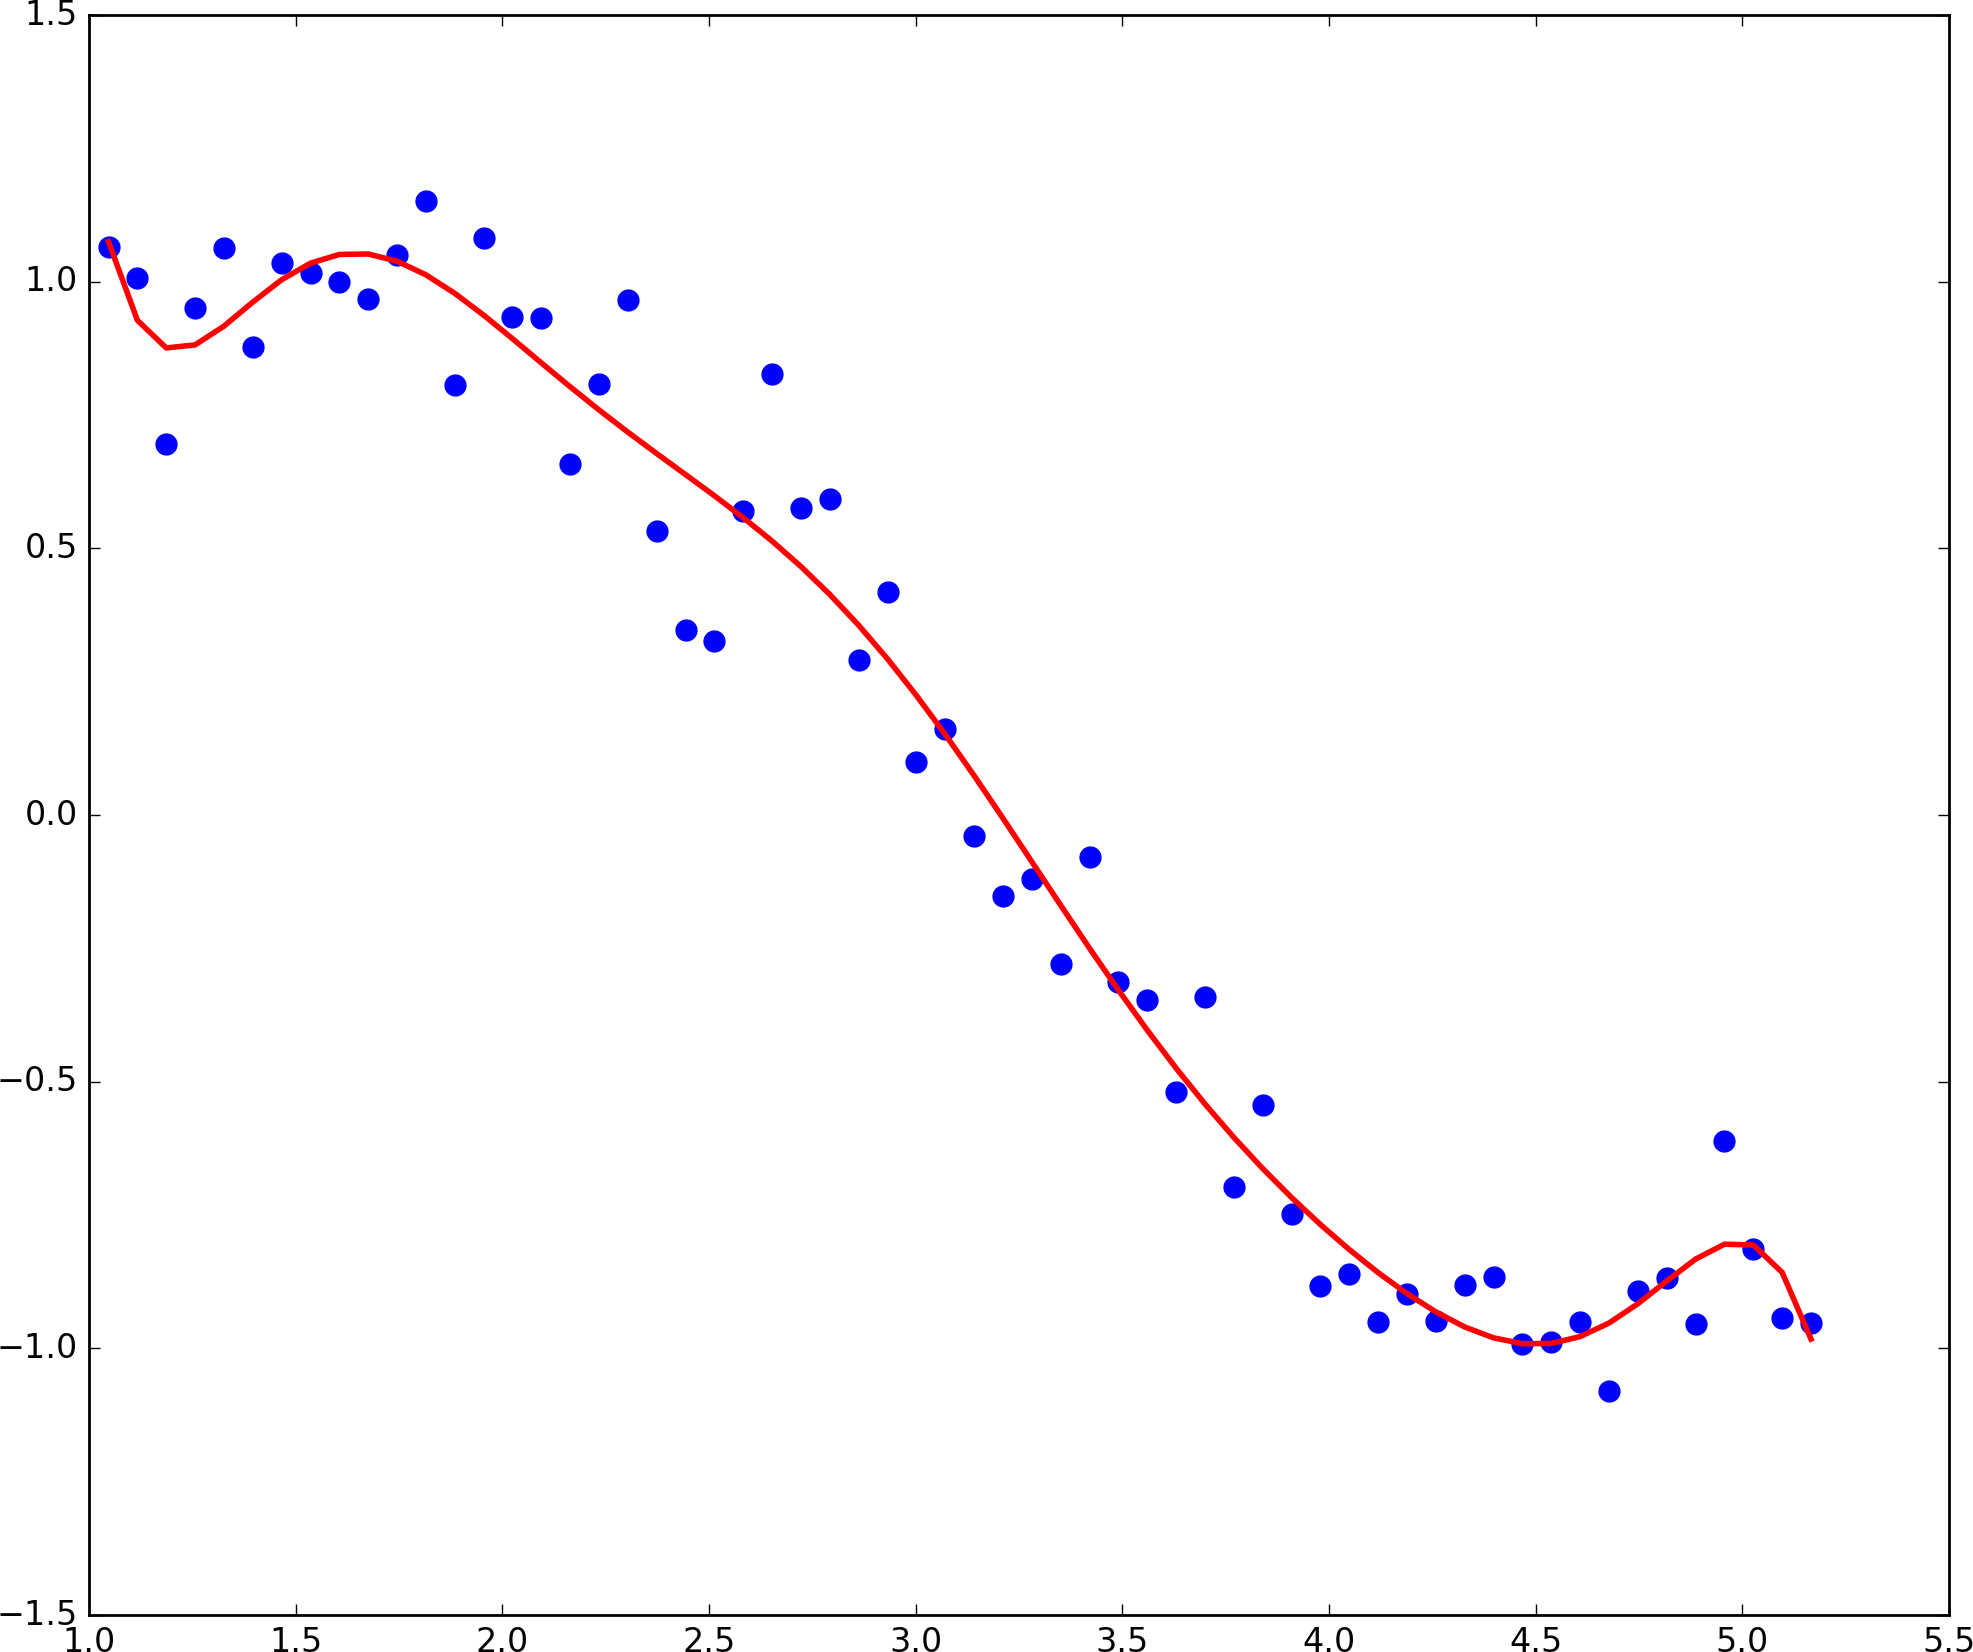
\includegraphics[width=0.99\textwidth]{./ridge_alpha1e-15.png}
\end{figure}
\vspace{-2em}
\begin{figure}
$\alpha=1e-2$
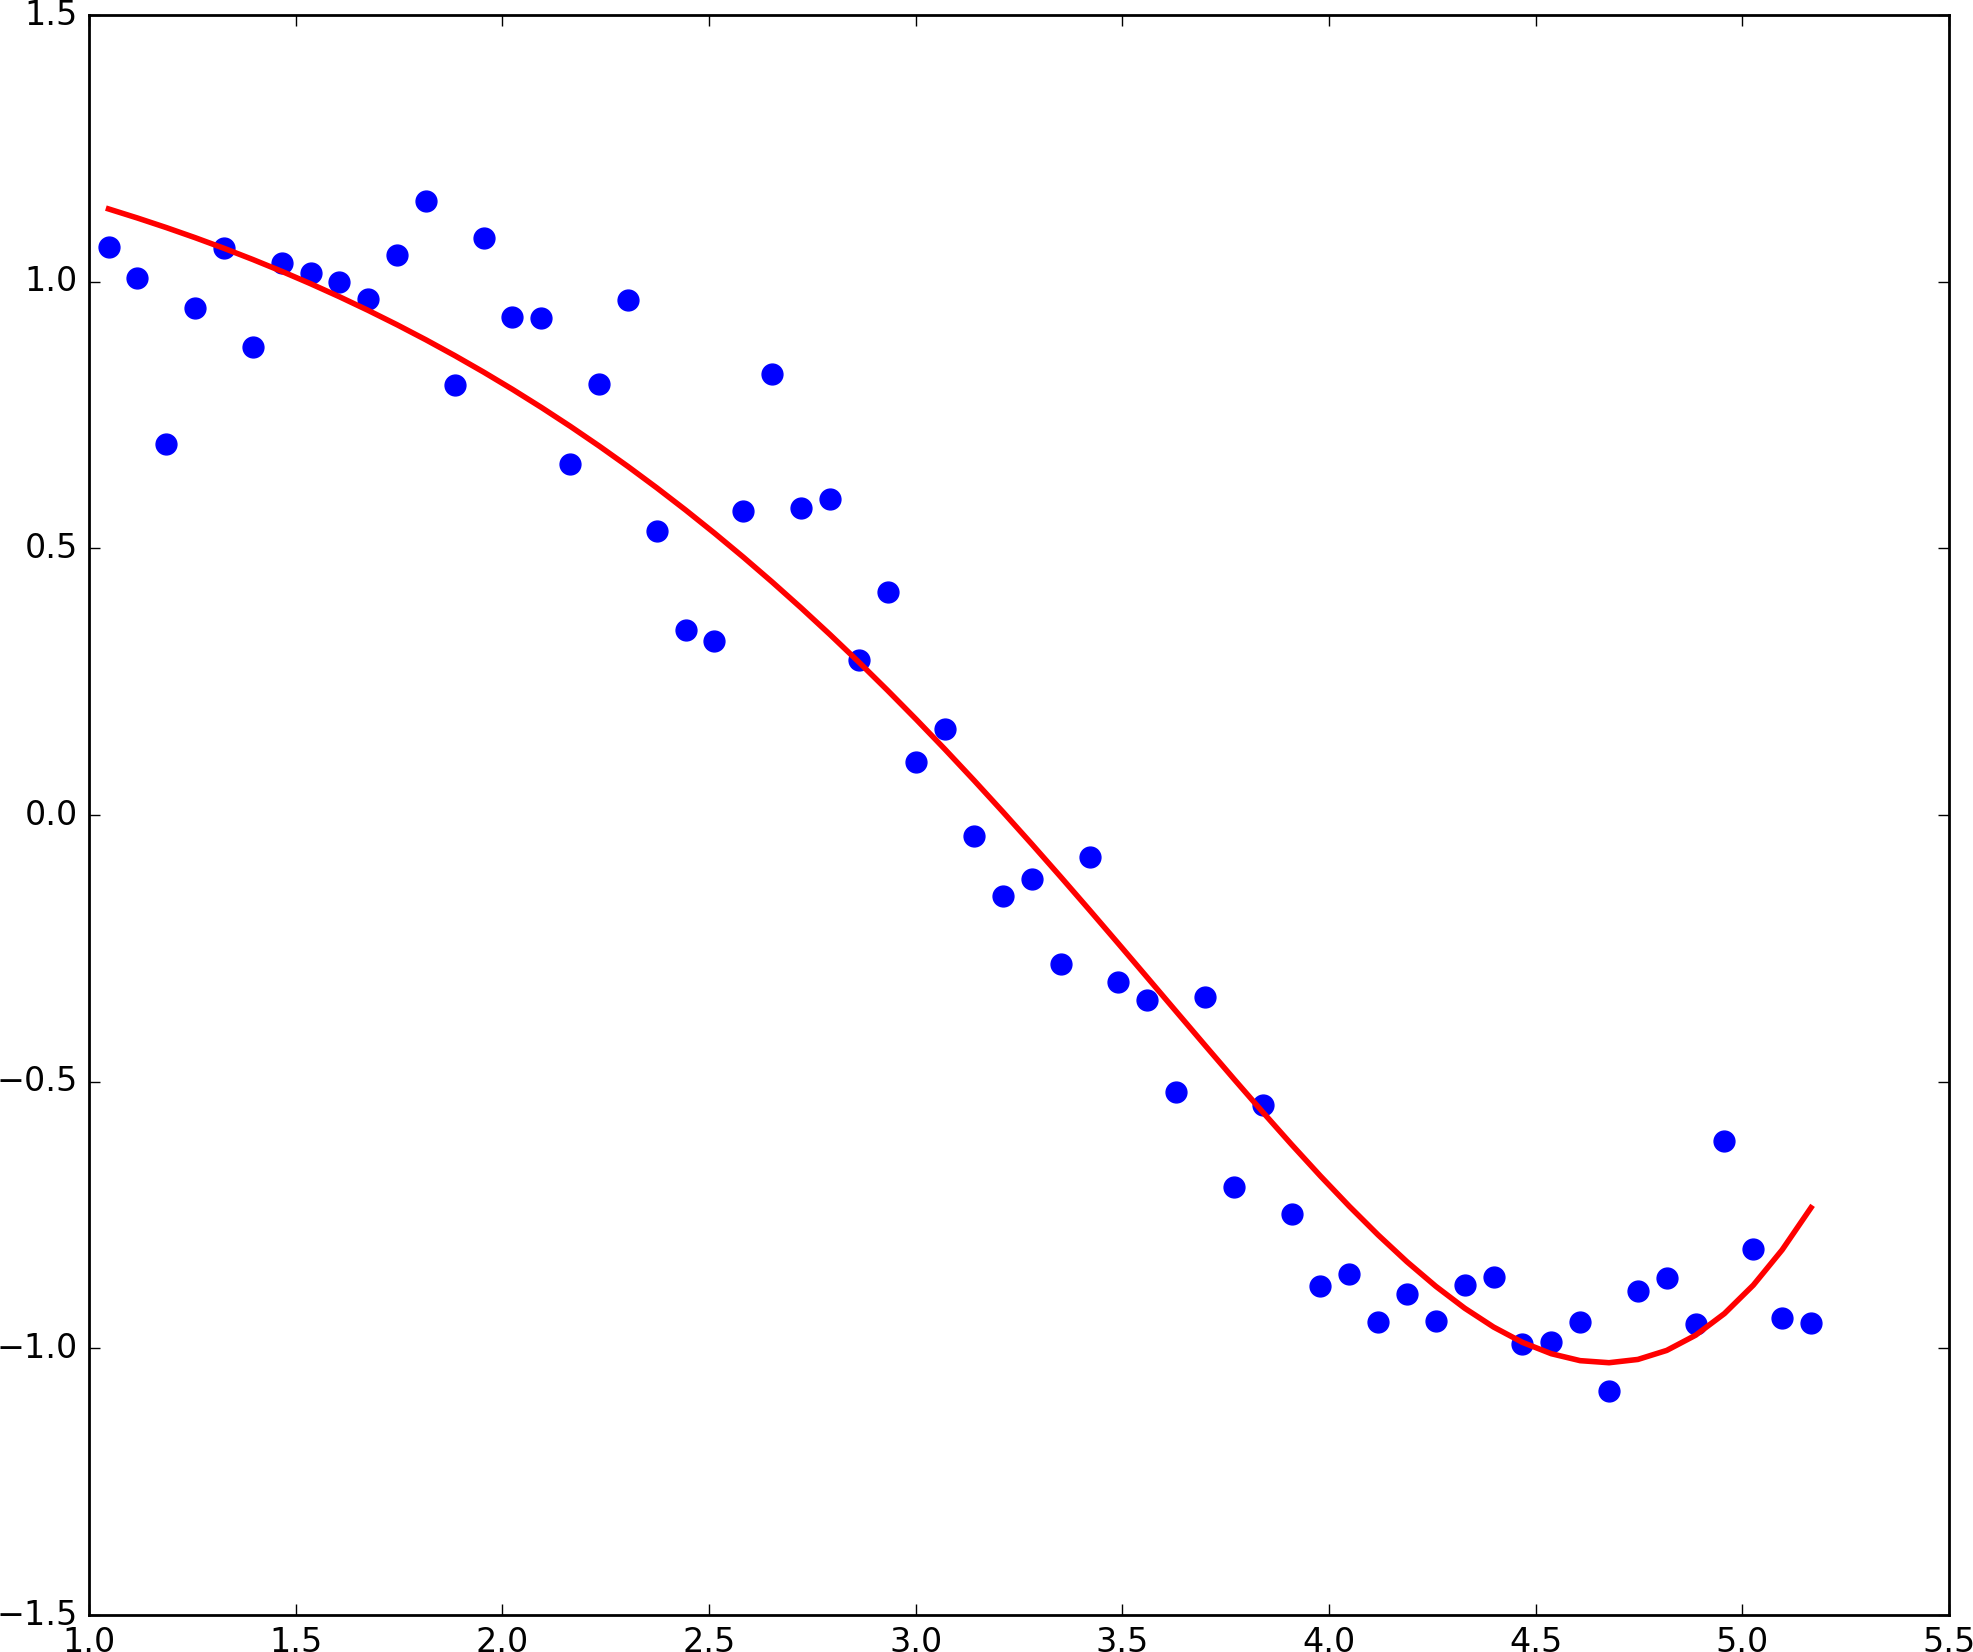
\includegraphics[width=0.99\textwidth]{./ridge_alpha1e-2.png}
\end{figure}
\column{.33\textwidth}
\vspace{-2em}
\begin{figure}
$\alpha=1e-4$
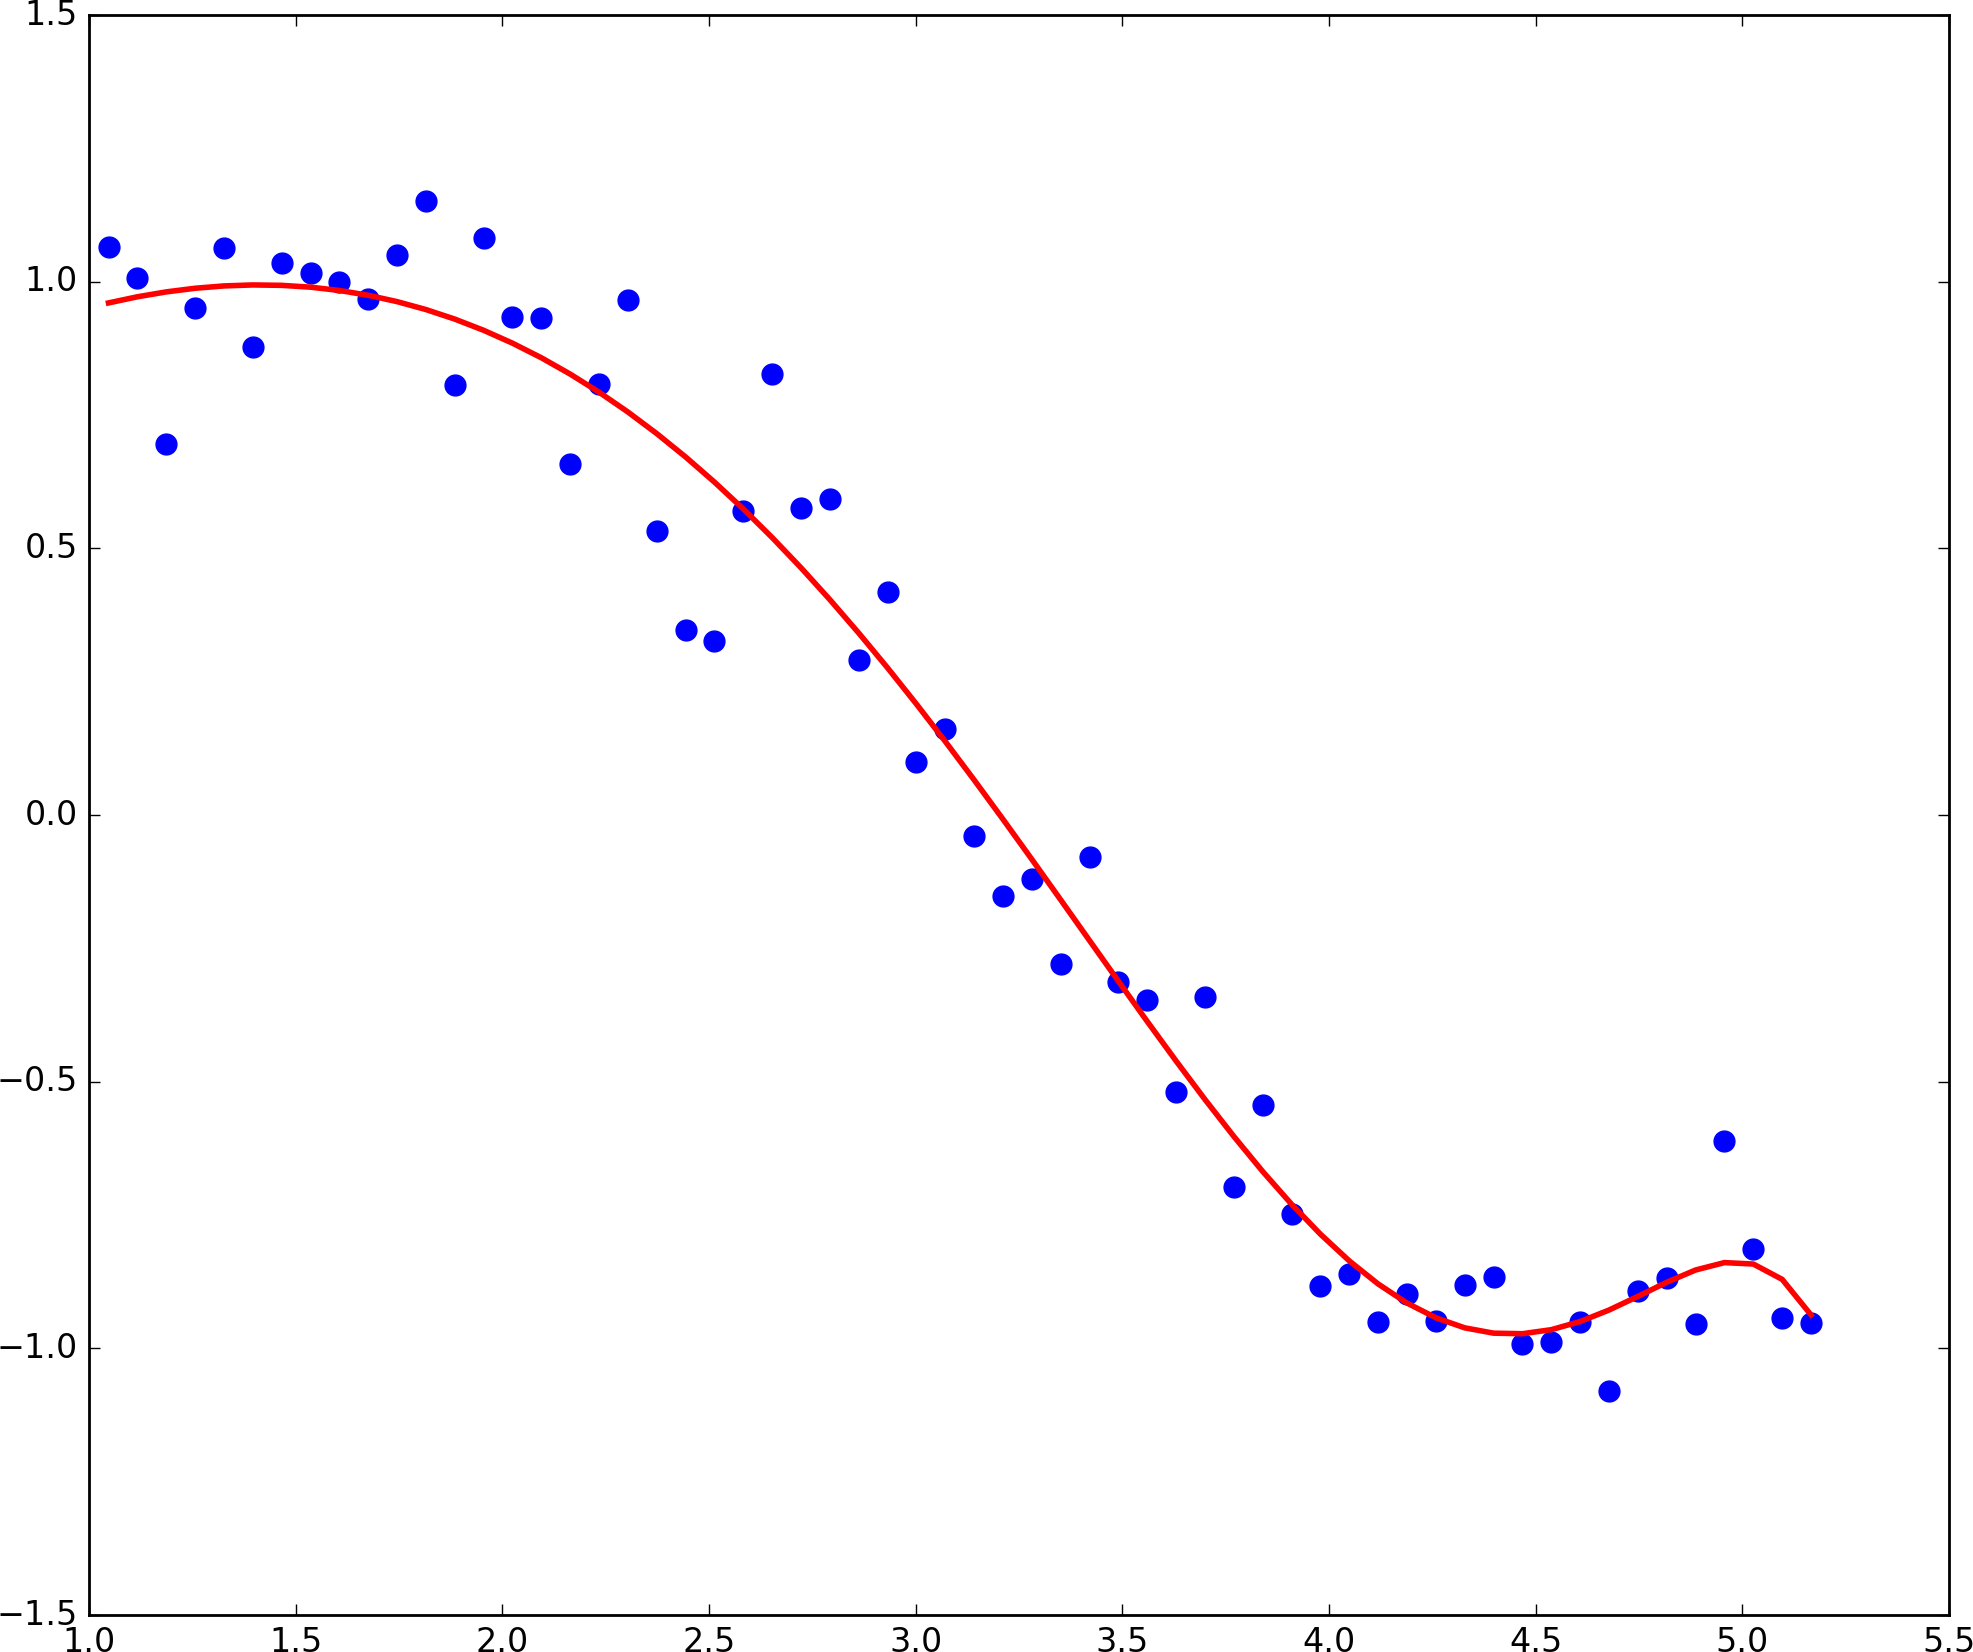
\includegraphics[width=0.99\textwidth]{./ridge_alpha1e-4.png}
\end{figure}
\vspace{-2em}
\begin{figure}
$\alpha=5$
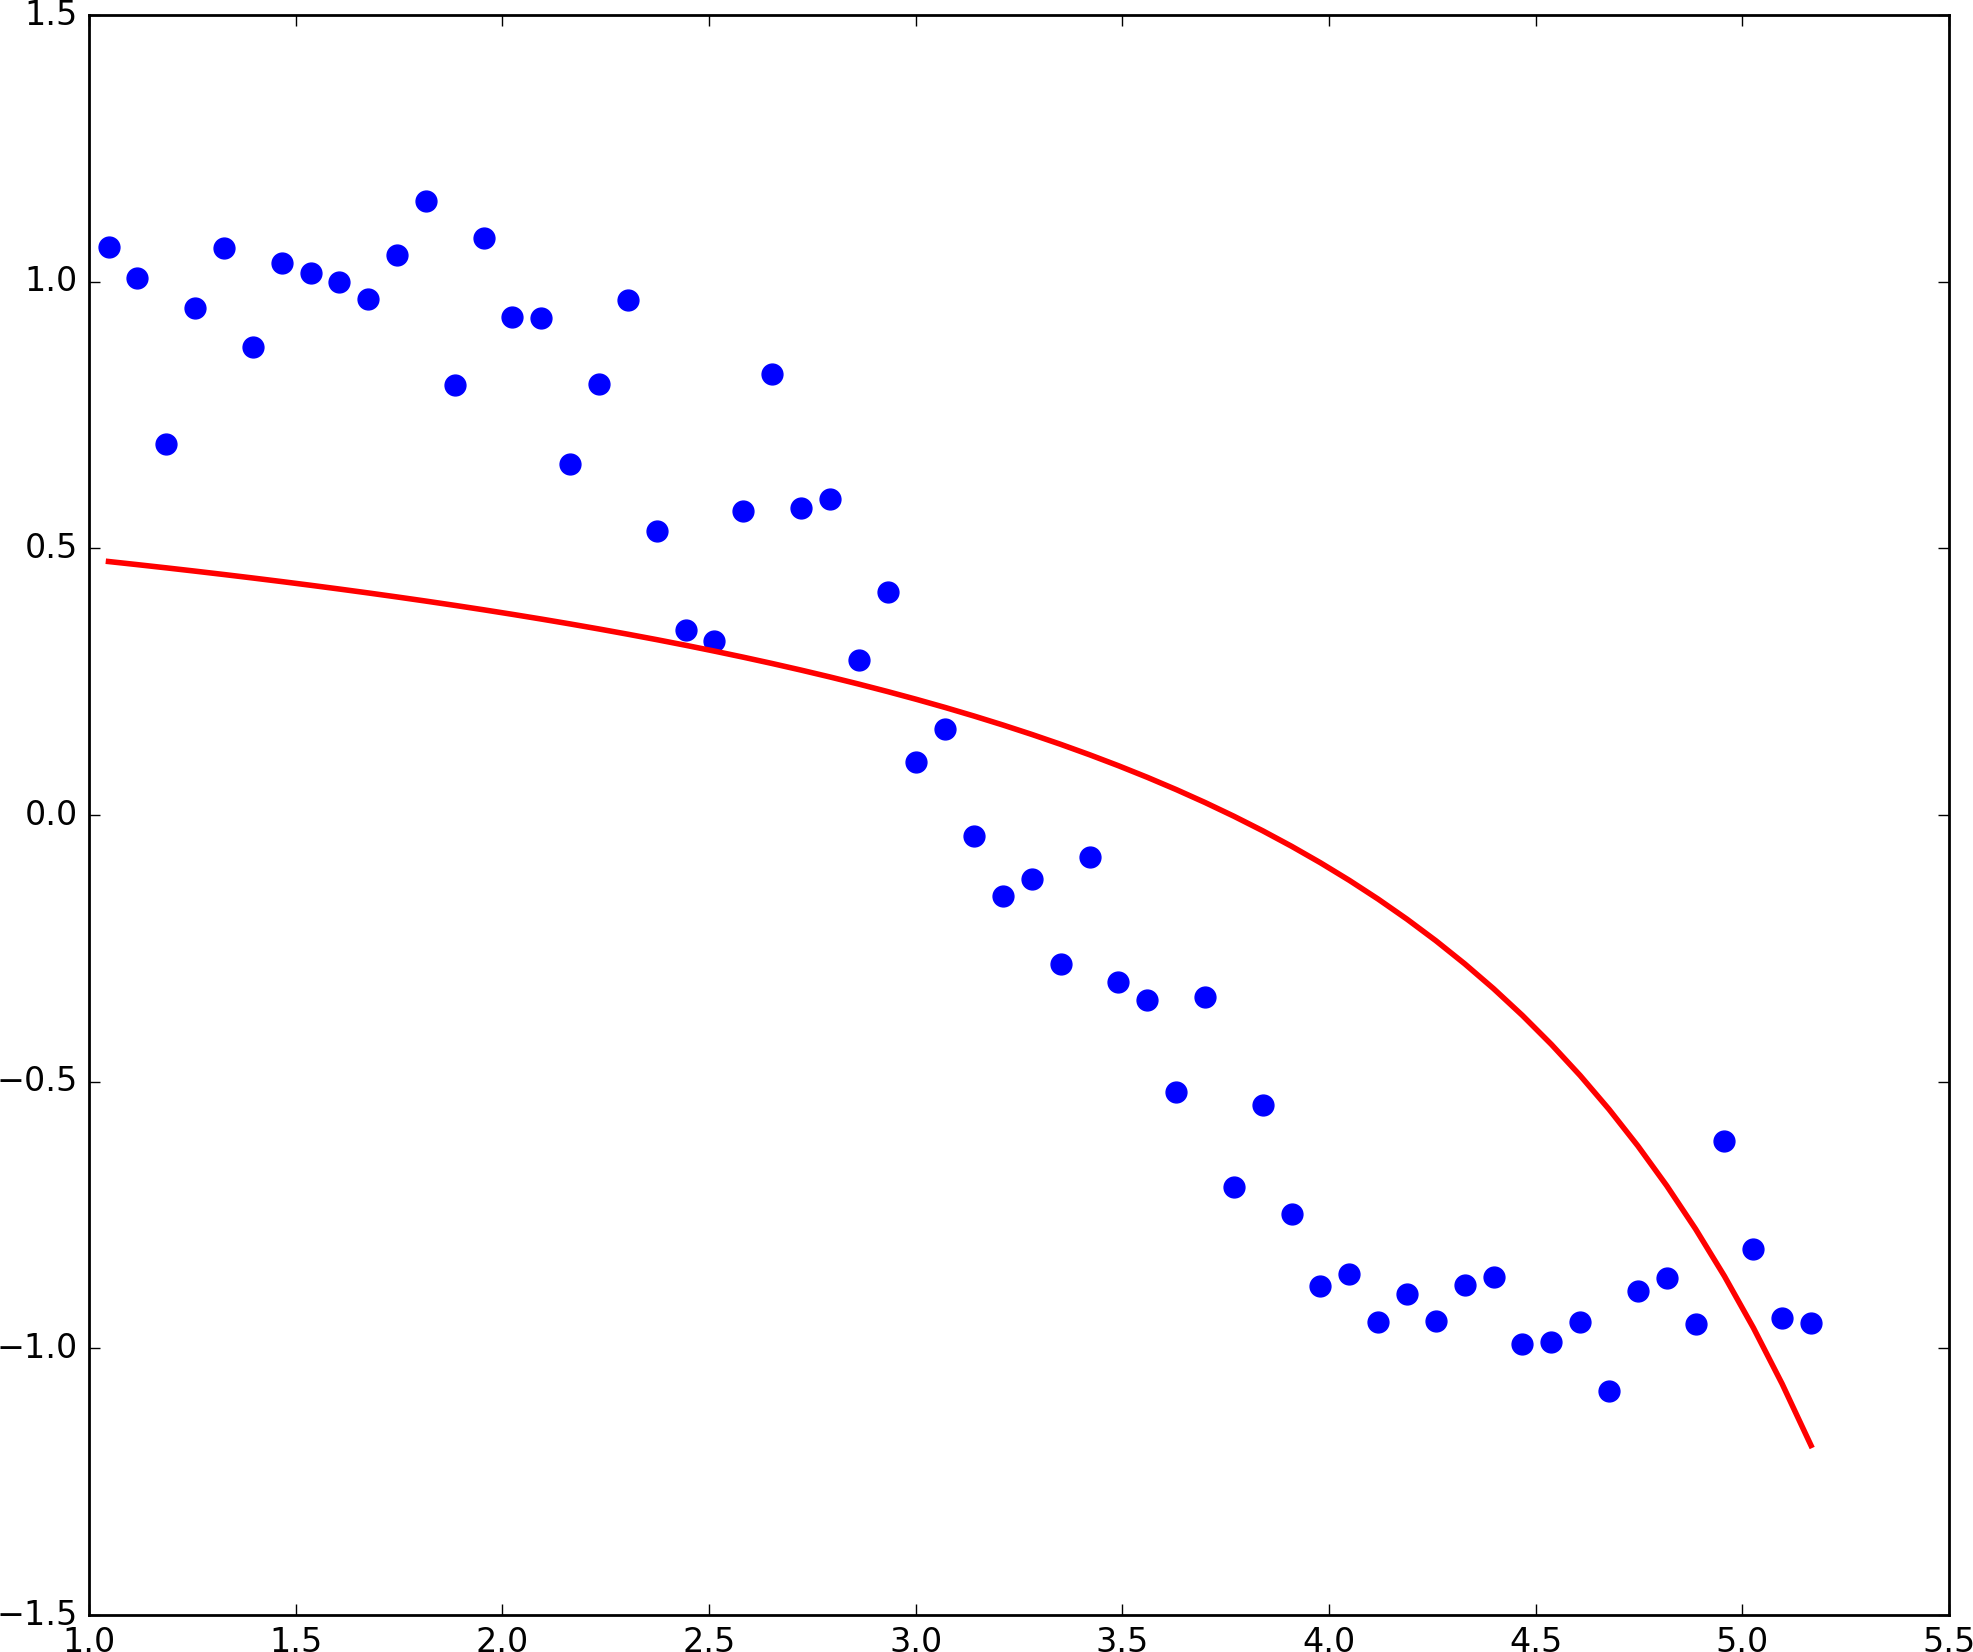
\includegraphics[width=0.99\textwidth]{./ridge_alpha5.png}
\end{figure}
\end{columns}
\end{frame}

%%%%%%%%%%%%%%%%%%%%%
\begin{frame}
\frametitle{Values of coefficients}
\vspace{-2em}
\begin{table}
\resizebox{\textwidth}{!}{%
\begin{tabular}{lllllllllll}
\toprule
{} &      rmse &      th\_0 &      th\_1 &      th\_2 &      th\_3 &      th\_4 &      th\_5 &      th\_6 &      th\_7 &      th\_8 \\
\midrule
alpha\_0      & +1.17e-02 & -3.62e+04 & +2.44e+05 & -7.46e+05 & +1.38e+06 & -1.71e+06 & +1.53e+06 & -1.00e+06 & +4.98e+05 & -1.88e+05 \\
alpha\_1e-15  & +1.46e-02 & +9.43e+01 & -2.98e+02 & +3.79e+02 & -2.37e+02 & +6.72e+01 & -2.60e-01 & -4.35e+00 & +5.62e-01 & +1.42e-01 \\
alpha\_1e-10  & +1.54e-02 & +1.12e+01 & -2.90e+01 & +3.11e+01 & -1.52e+01 & +2.89e+00 & +1.69e-01 & -9.10e-02 & -1.08e-02 & +1.98e-03 \\
alpha\_1e-08  & +1.58e-02 & +1.34e+00 & -1.53e+00 & +1.75e+00 & -6.80e-01 & +3.88e-02 & +1.58e-02 & +1.59e-04 & -3.60e-04 & -5.37e-05 \\
alpha\_0.0001 & +1.60e-02 & +5.61e-01 & +5.47e-01 & -1.28e-01 & -2.57e-02 & -2.82e-03 & -1.10e-04 & +4.06e-05 & +1.52e-05 & +3.65e-06 \\
alpha\_0.001  & +1.67e-02 & +8.18e-01 & +3.05e-01 & -8.67e-02 & -2.05e-02 & -2.84e-03 & -2.19e-04 & +1.81e-05 & +1.24e-05 & +3.43e-06 \\
alpha\_0.01   & +2.39e-02 & +1.30e+00 & -8.84e-02 & -5.15e-02 & -1.01e-02 & -1.41e-03 & -1.32e-04 & +7.23e-07 & +4.14e-06 & +1.30e-06 \\
alpha\_1      & +9.41e-02 & +9.69e-01 & -1.39e-01 & -1.93e-02 & -3.00e-03 & -4.66e-04 & -6.97e-05 & -9.90e-06 & -1.29e-06 & -1.43e-07 \\
alpha\_5      & +2.31e-01 & +5.48e-01 & -5.89e-02 & -8.52e-03 & -1.42e-03 & -2.41e-04 & -4.08e-05 & -6.87e-06 & -1.15e-06 & -1.91e-07 \\
alpha\_10     & +3.00e-01 & +4.00e-01 & -3.72e-02 & -5.53e-03 & -9.50e-04 & -1.67e-04 & -2.96e-05 & -5.23e-06 & -9.25e-07 & -1.63e-07 \\
alpha\_20     & +3.79e-01 & +2.77e-01 & -2.25e-02 & -3.40e-03 & -5.99e-04 & -1.08e-04 & -1.97e-05 & -3.60e-06 & -6.58e-07 & -1.20e-07 \\
\bottomrule
\end{tabular}
}
\end{table}
\begin{figure}
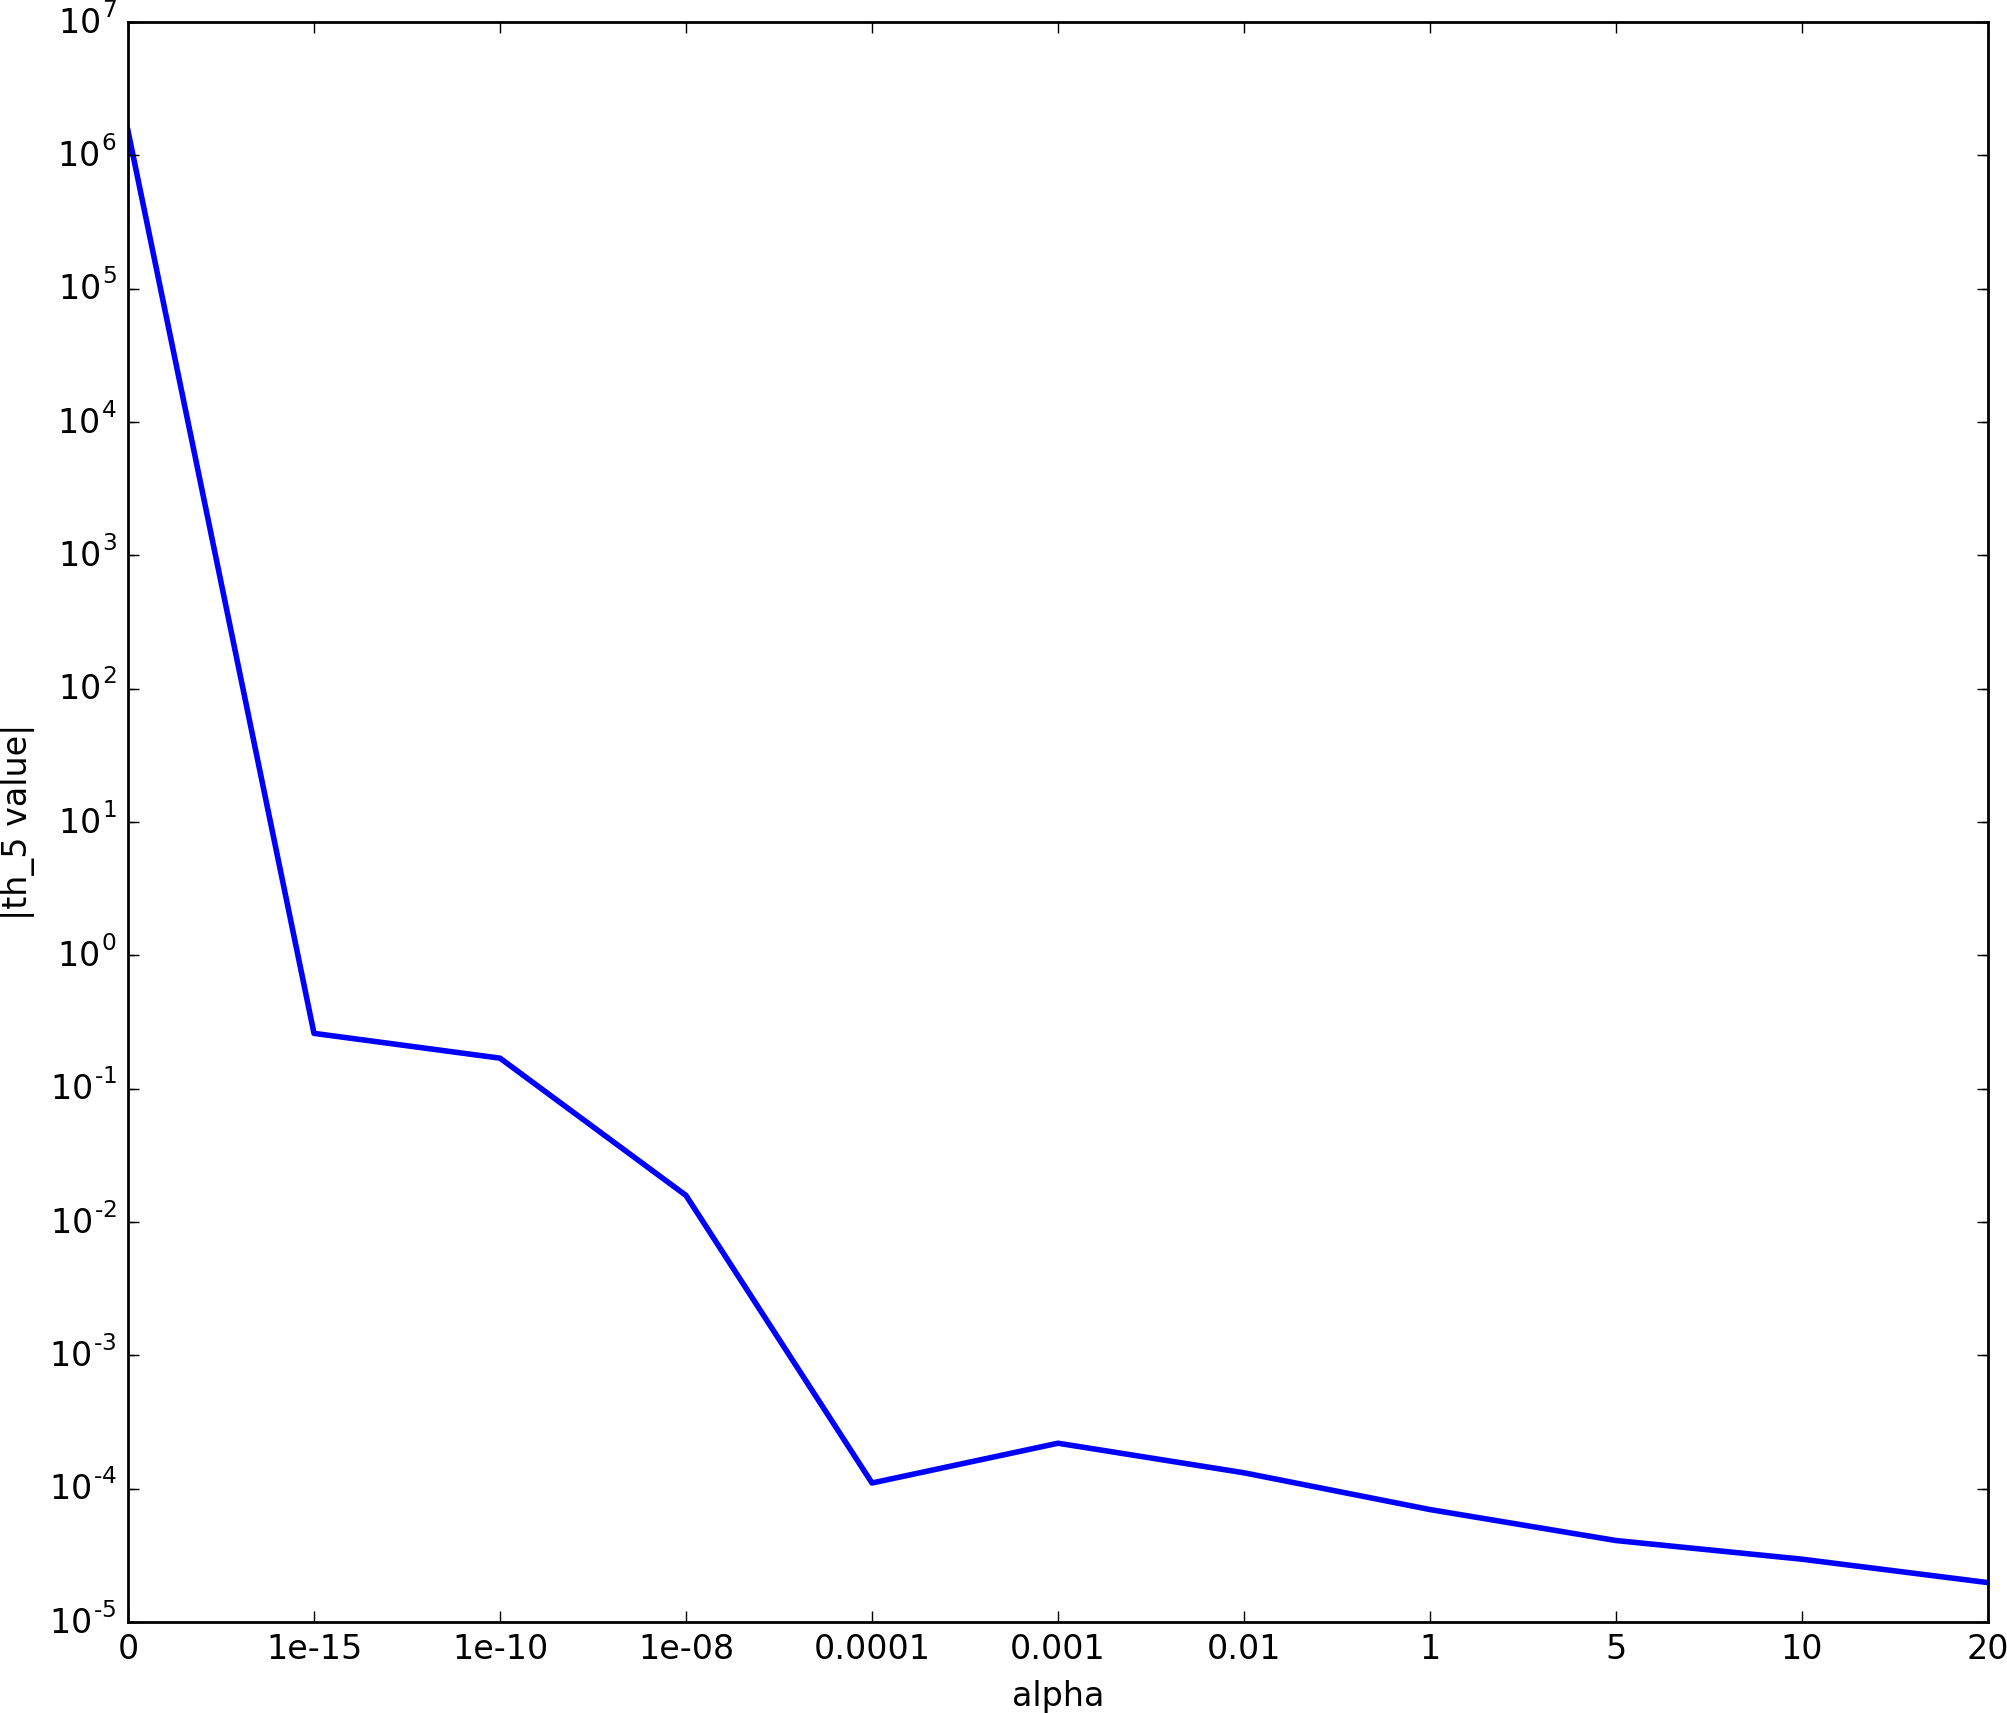
\includegraphics[height=0.4\textheight]{./coefs_th5_ridge.png}\\
Value of $\theta_5$
\end{figure}
\end{frame}

%%%%%%%%%%%%%%%%%
\begin{frame}
\frametitle{Determination of the parameters in the ridge regression}
Considering the cost function J:
$$
J(\bm{\theta}) =J_{lms}(\bm{\theta}) + \alpha \sum_{i=0}^p \theta_i^2
$$
In a gradient algorithm, update of the parameters:

$\theta^{k+1}_i = \theta^k_i - \nu.(\frac{\partial J_{lms}}{D\theta_i} - 2\alpha\theta^k_i)$

So the update rule is:
$$
\theta^{k+1}_i = \theta^k_i(1-2 \nu \alpha) - \Delta_{lms}
$$
where
$\Delta_{lms}$ is the update in case of non-regularized regression

\end{frame}


%%%%%%%%%%%%%%%%%%%%
\begin{frame}
\frametitle{Lasso regression (L1)}
\begin{block}{}
Lasso regression is a linear regression with a Lasso regularization:
$$
J(\bm{\theta}) = \frac{1}{n} \sum (y_i - h_{\bm{\theta}}(x_i))^2 + \alpha \sum_{i=0}^p |\theta_i|
$$
\end{block}
\end{frame}

%%%%%%%%%%%%%%%%%%%%
\begin{frame}
\frametitle{Results for $p=15$ and varying $\alpha$}
\begin{columns}
\column{.33\textwidth}
\vspace{-2em}
\begin{figure}
$\alpha=0$
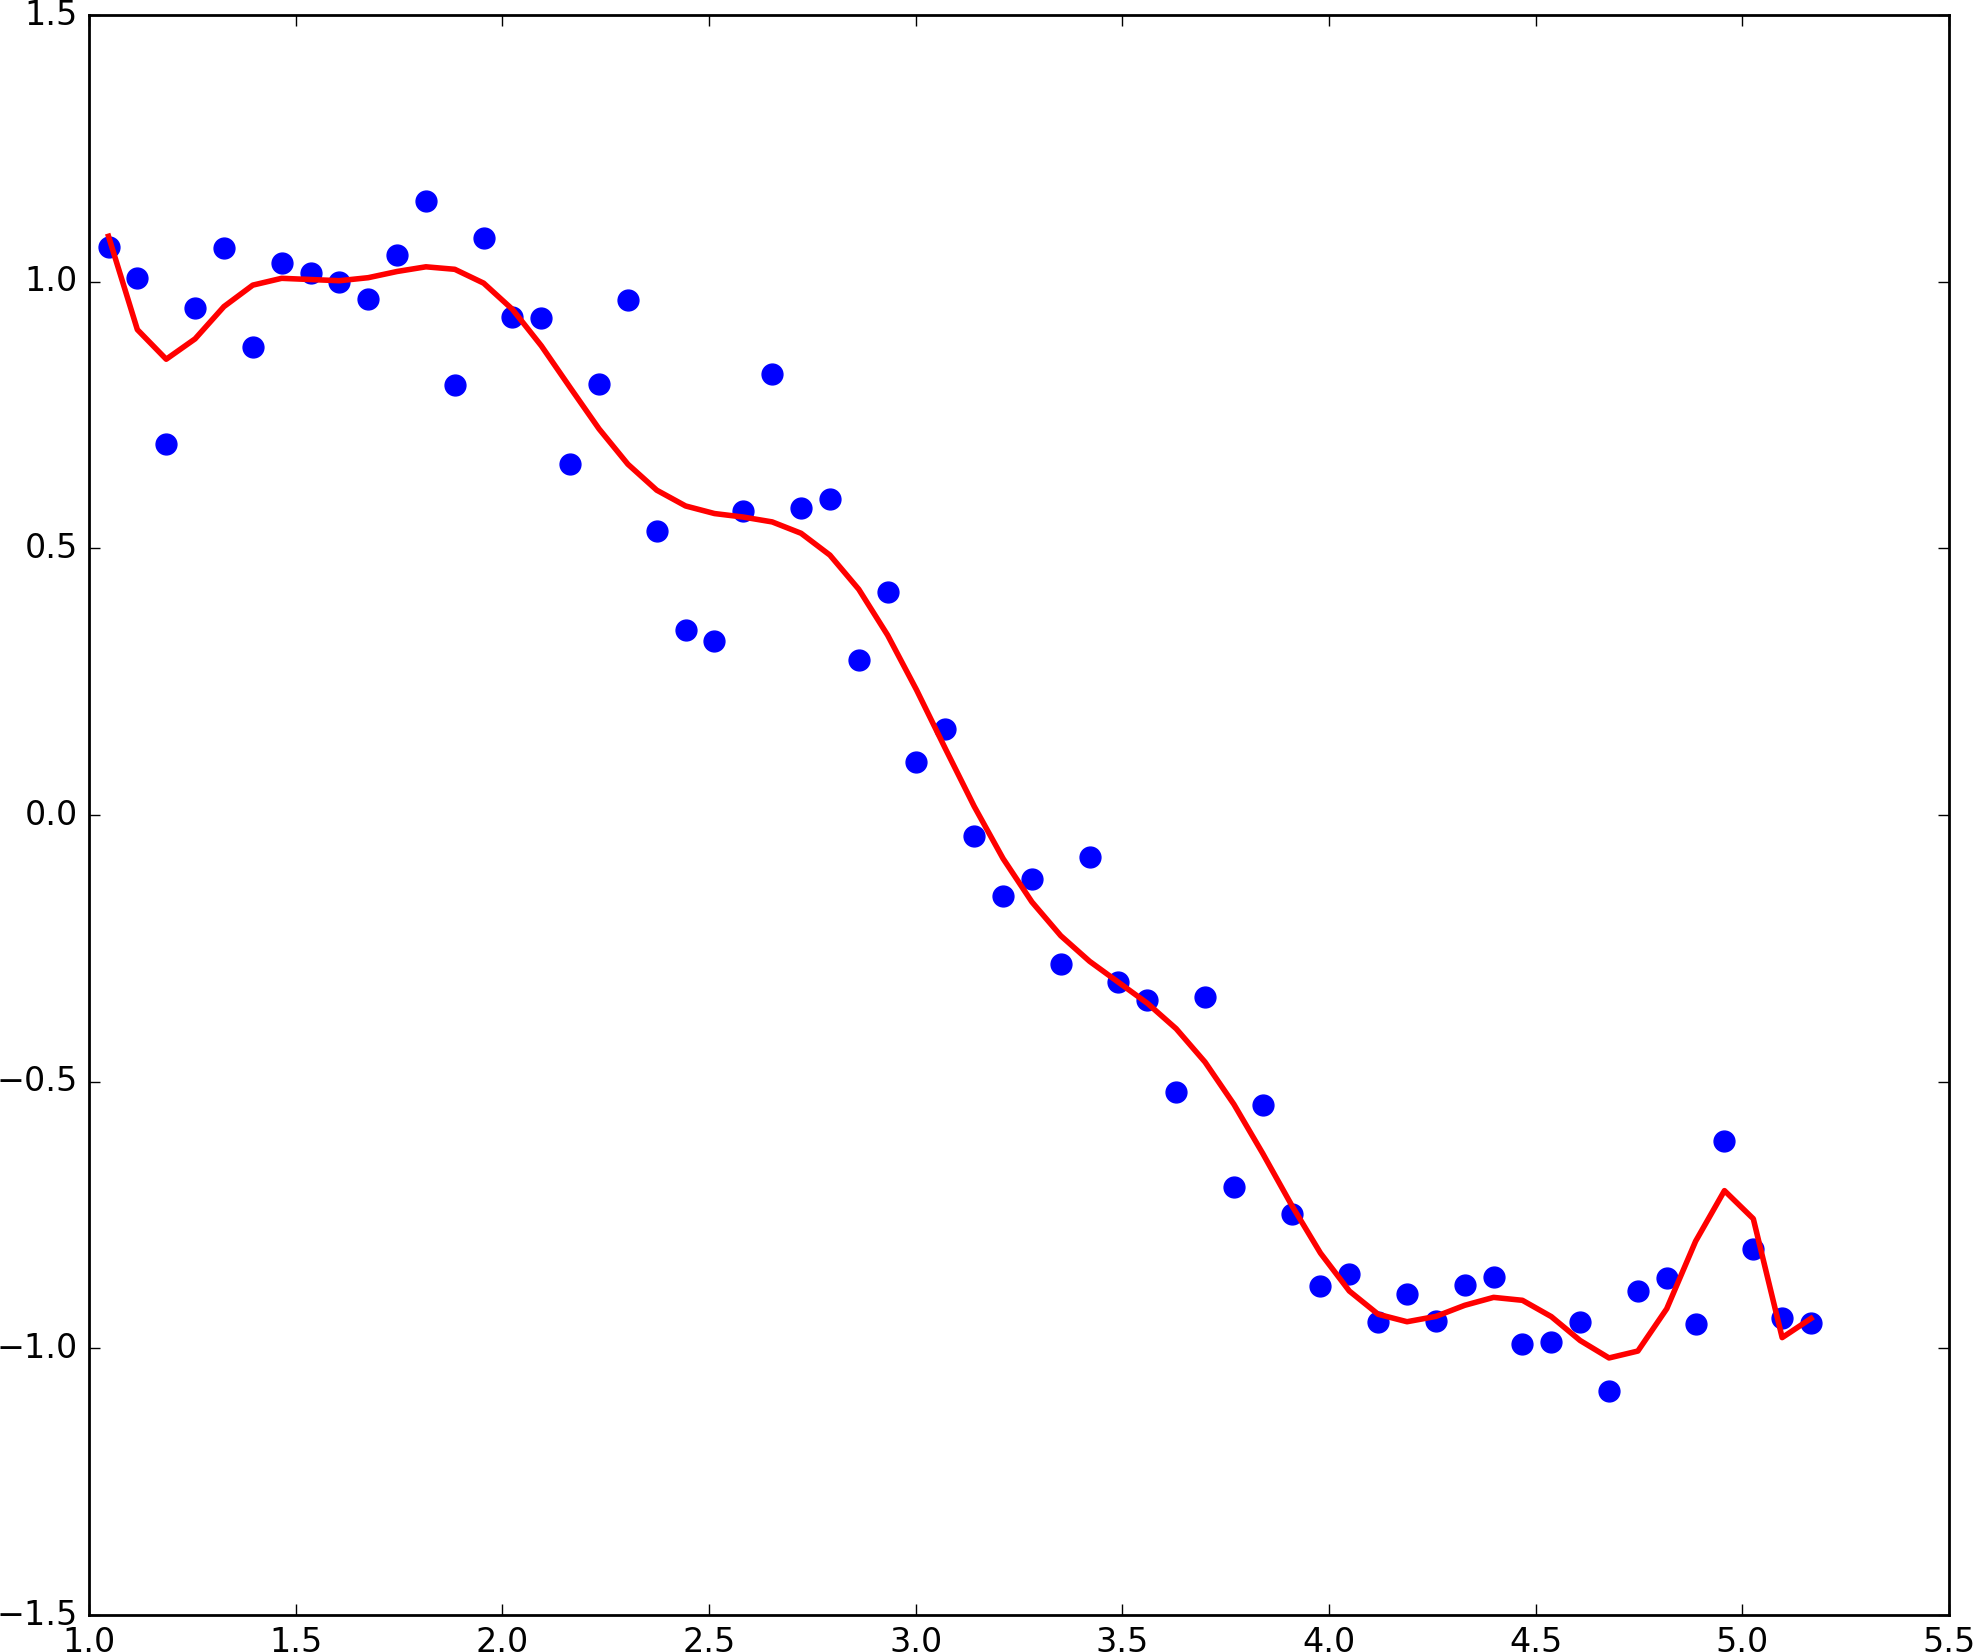
\includegraphics[width=0.99\textwidth]{./lasso_alpha0.png}
\end{figure}
\vspace{-2em}
\begin{figure}
$\alpha=1e-3$
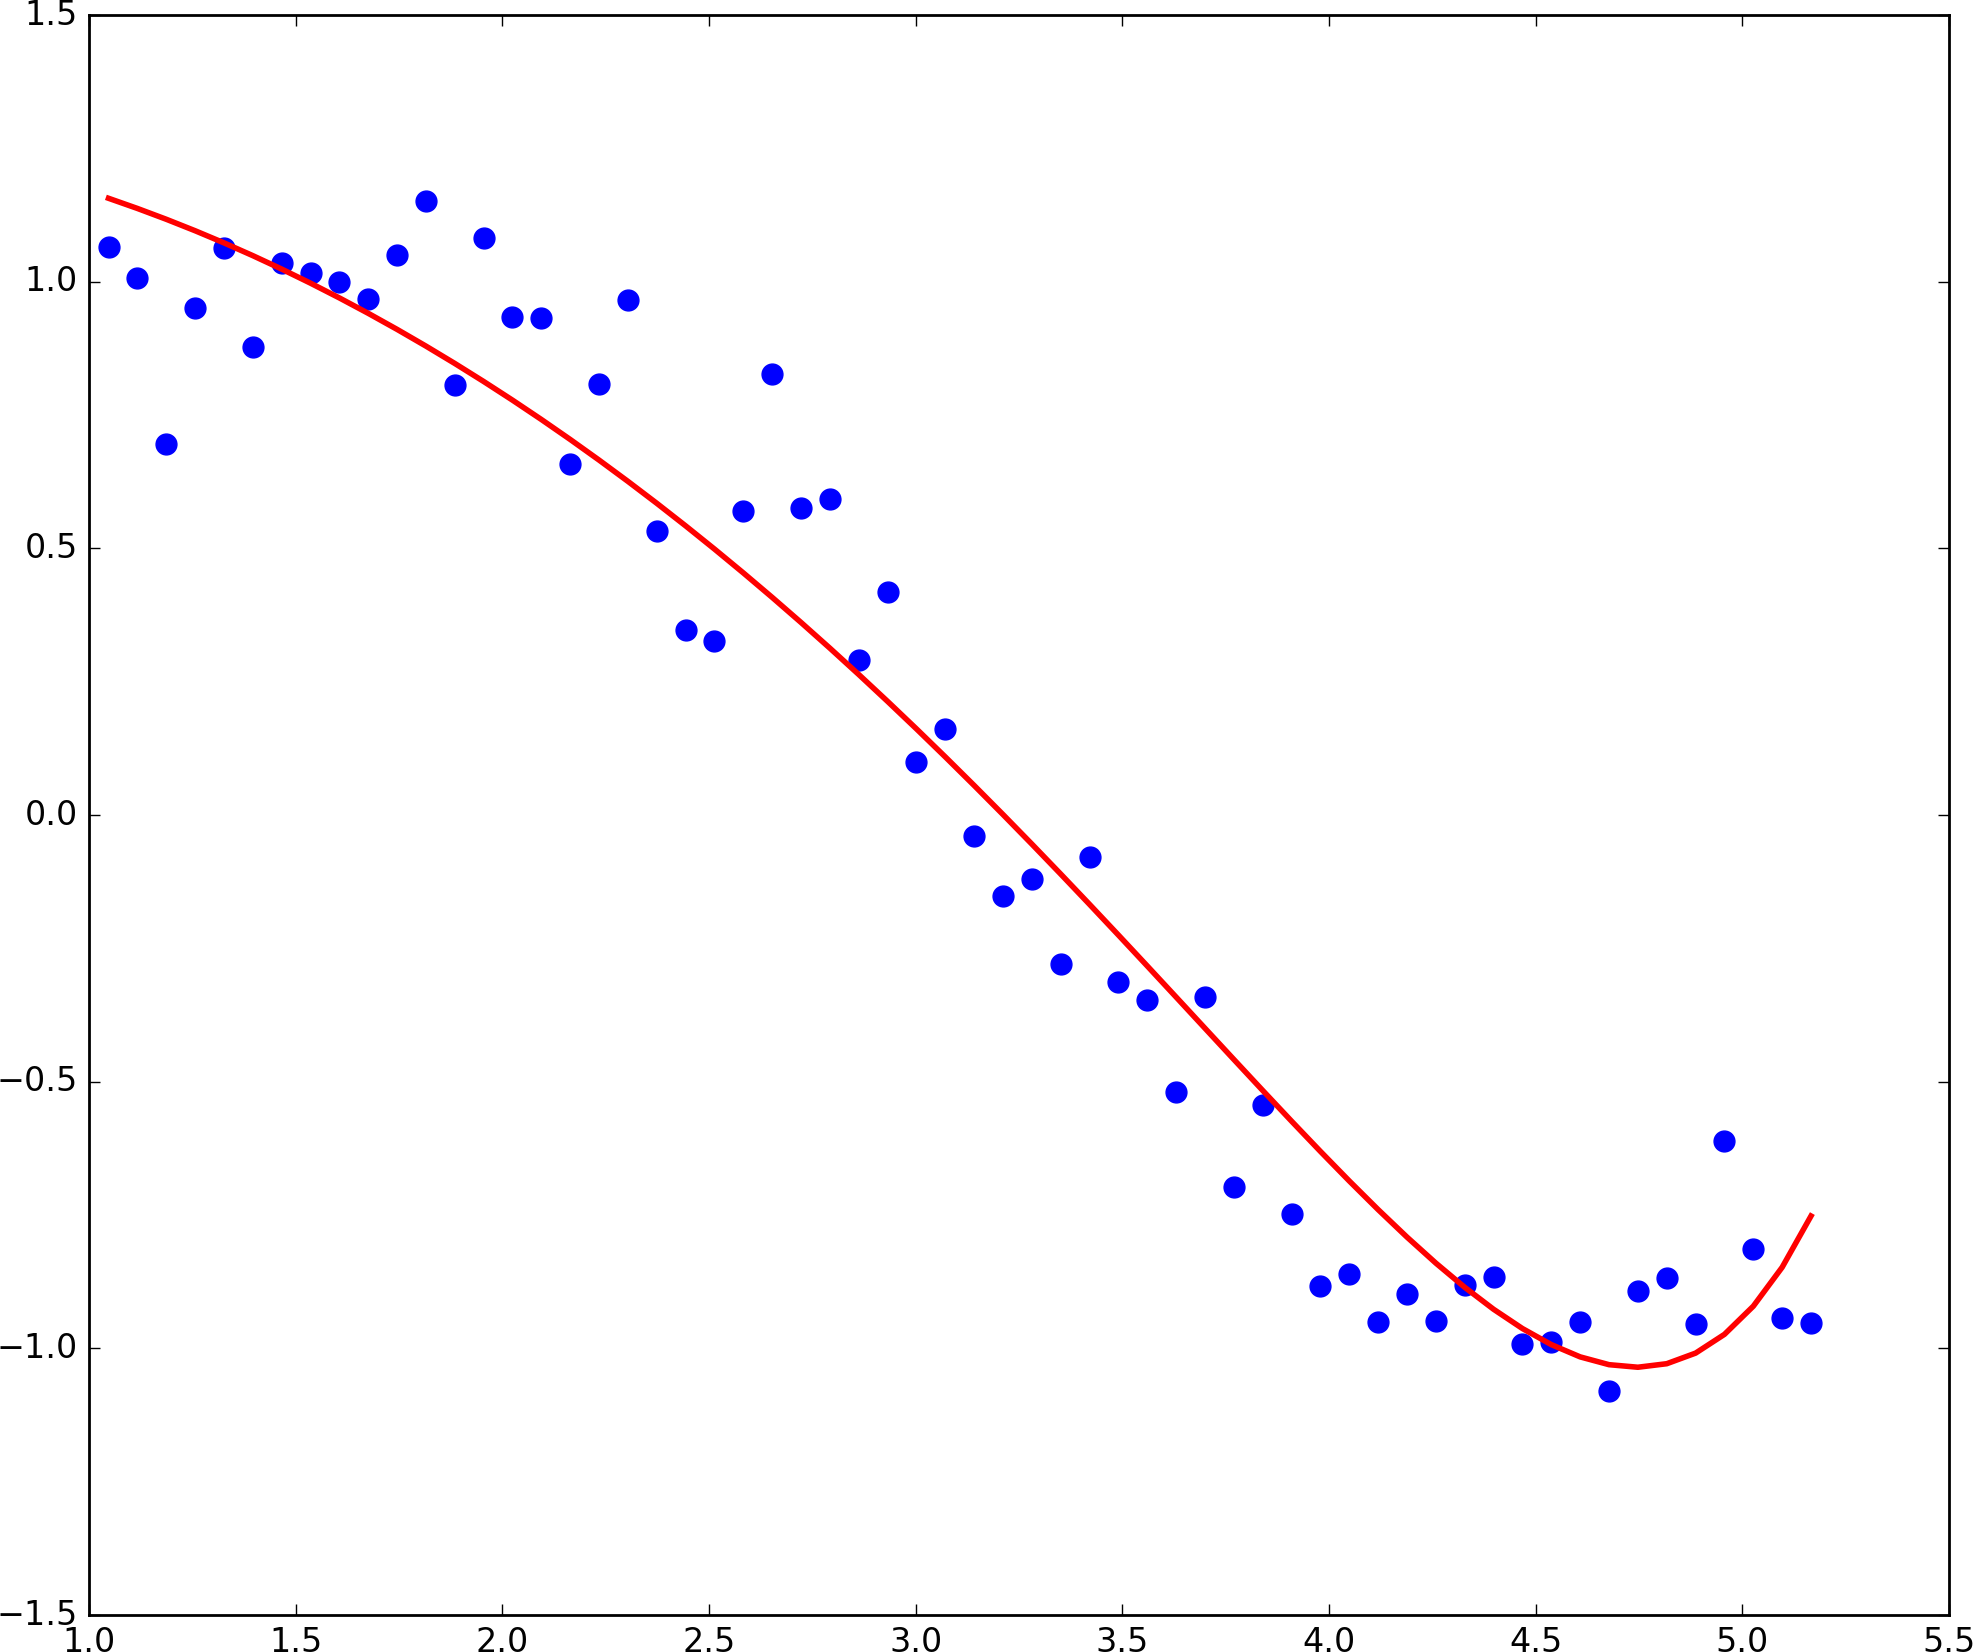
\includegraphics[width=0.99\textwidth]{./lasso_alpha1e-3.png}
\end{figure}
\column{.33\textwidth}
\vspace{-2em}
\begin{figure}
$\alpha=1e-15$
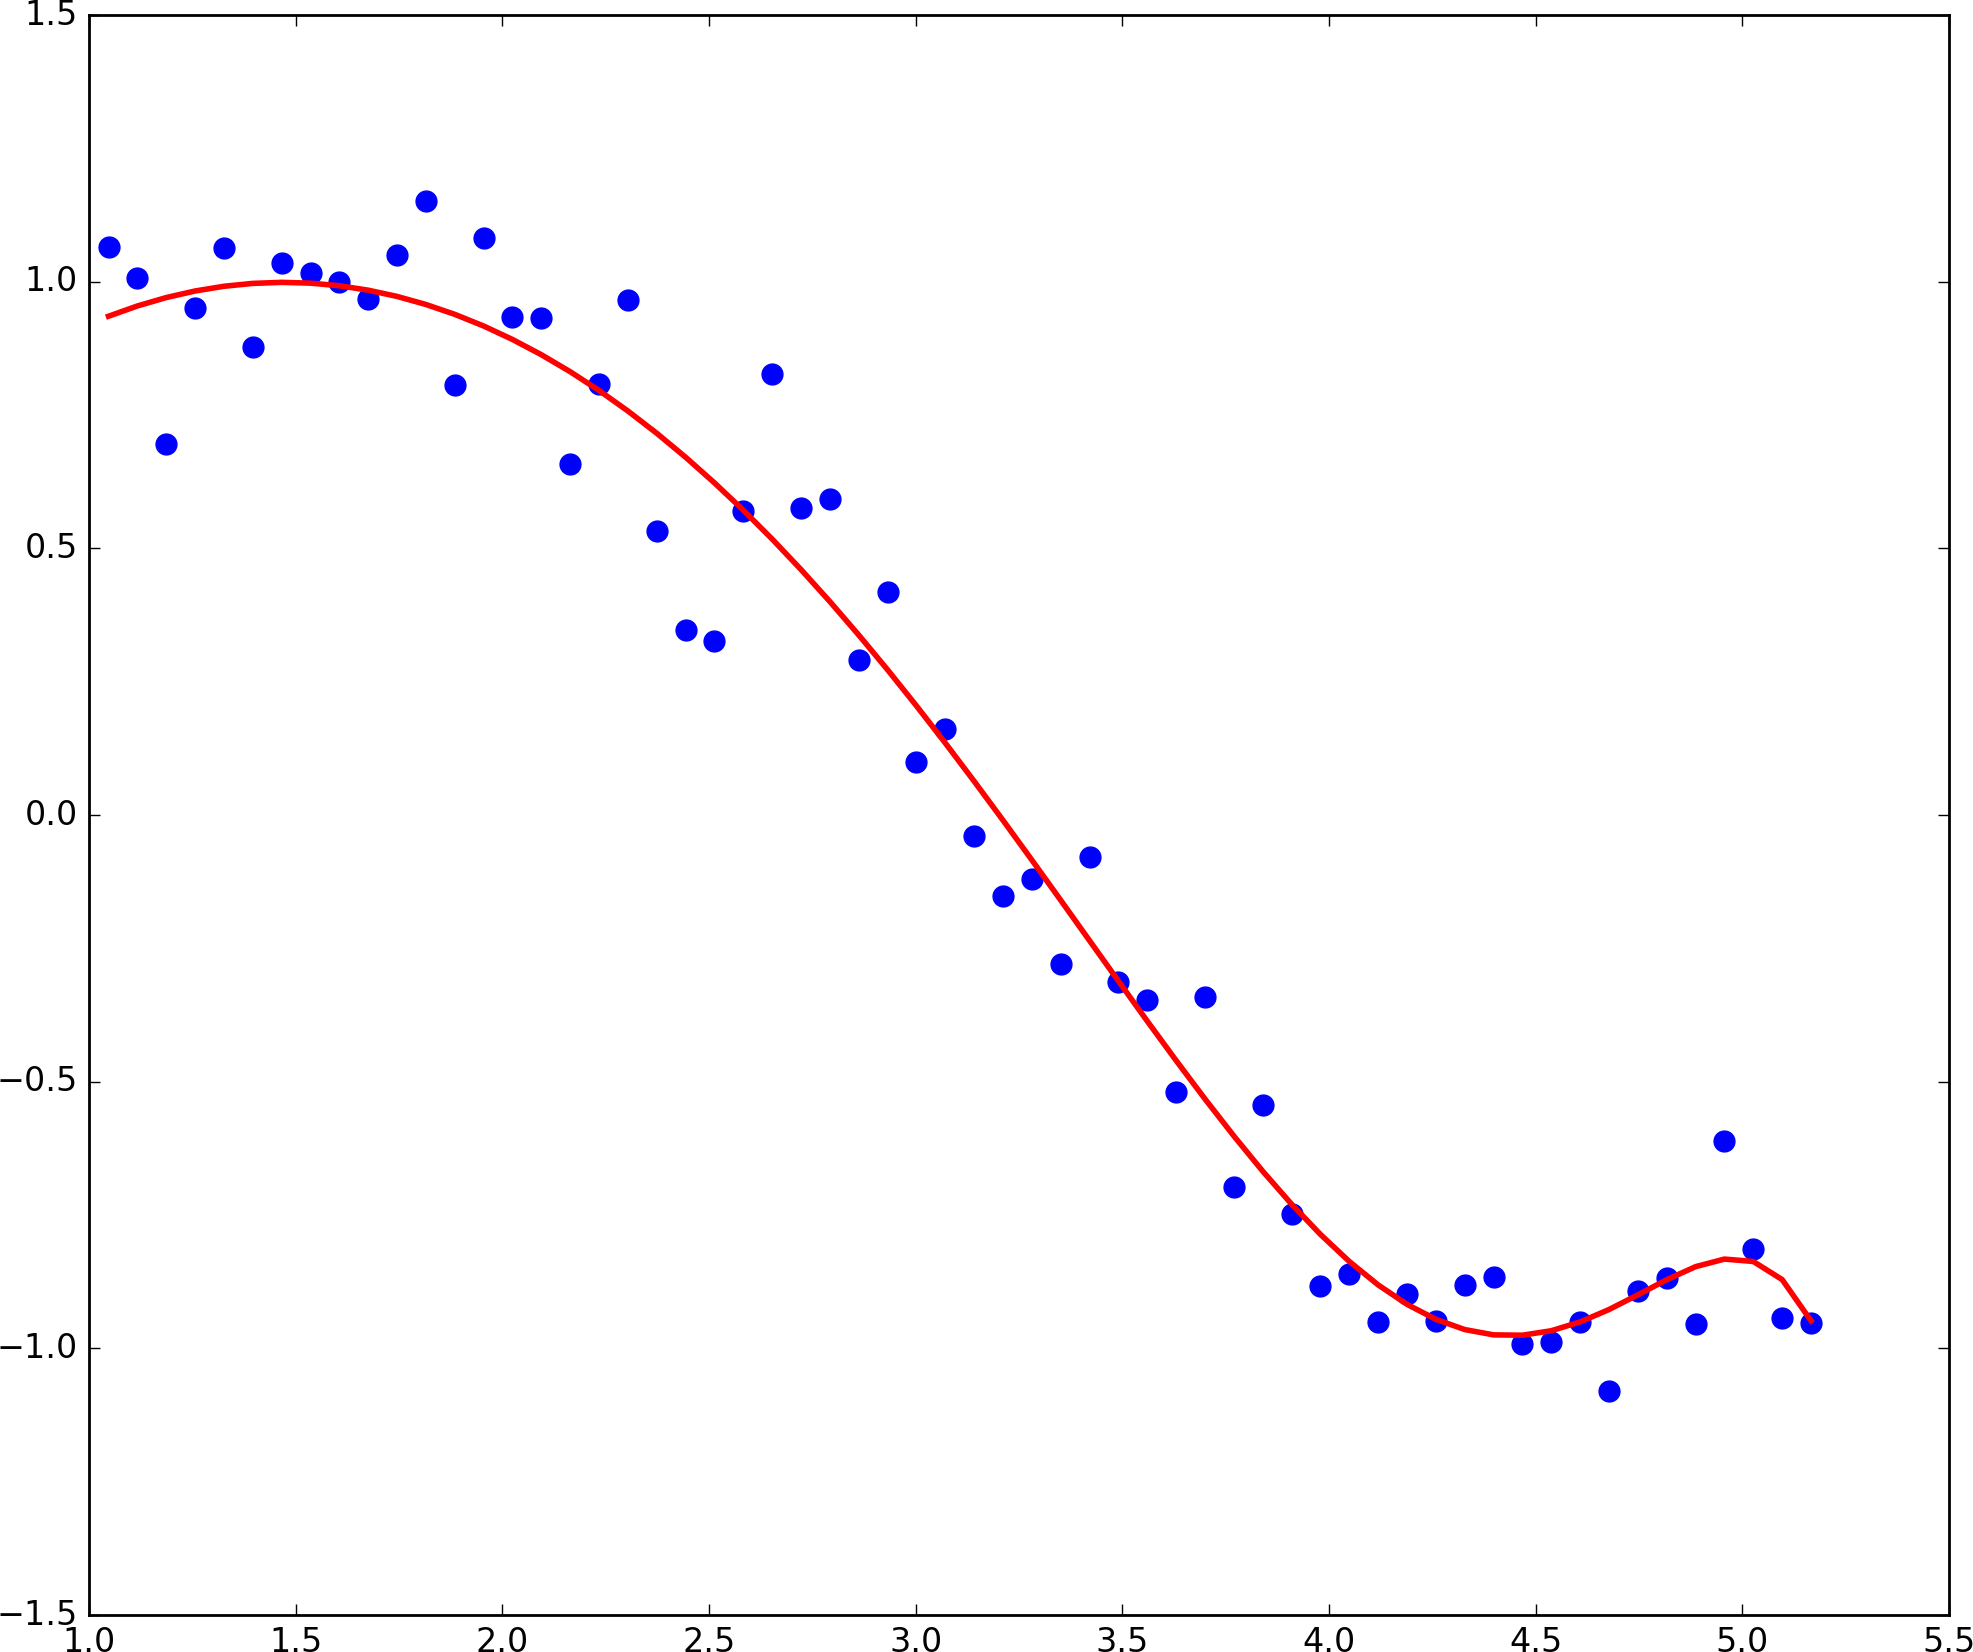
\includegraphics[width=0.99\textwidth]{./lasso_alpha1e-15.png}
\end{figure}
\vspace{-2em}
\begin{figure}
$\alpha=1e-2$
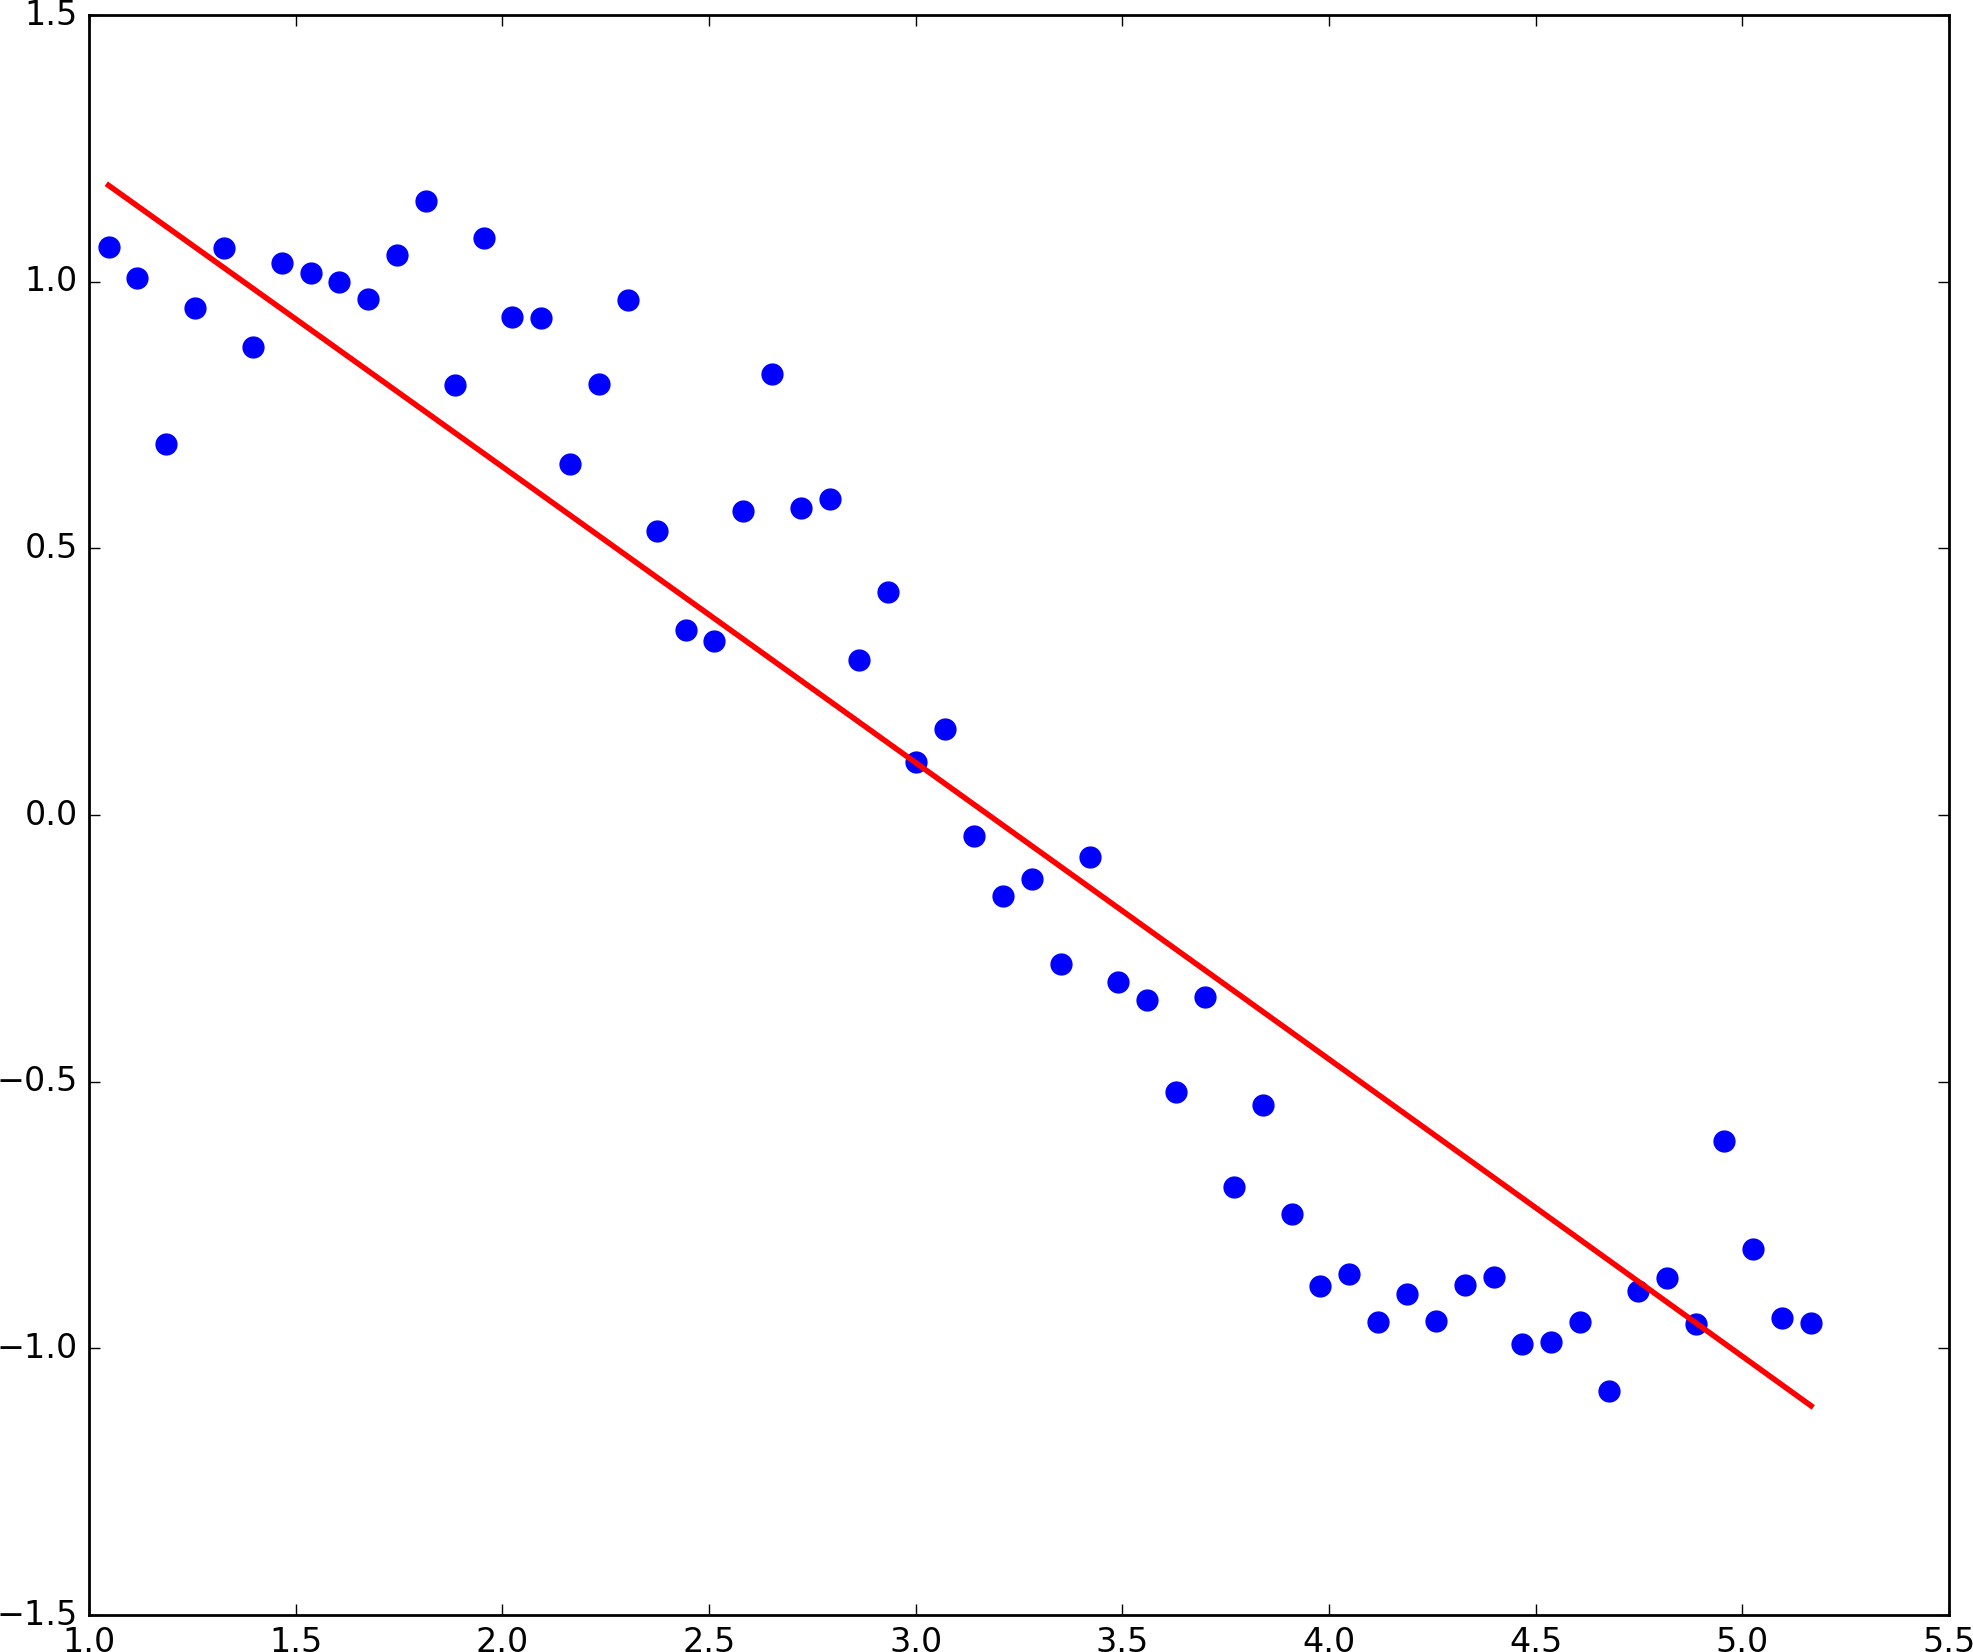
\includegraphics[width=0.99\textwidth]{./lasso_alpha1e-2.png}
\end{figure}
\column{.33\textwidth}
\vspace{-2em}
\begin{figure}
$\alpha=1e-4$
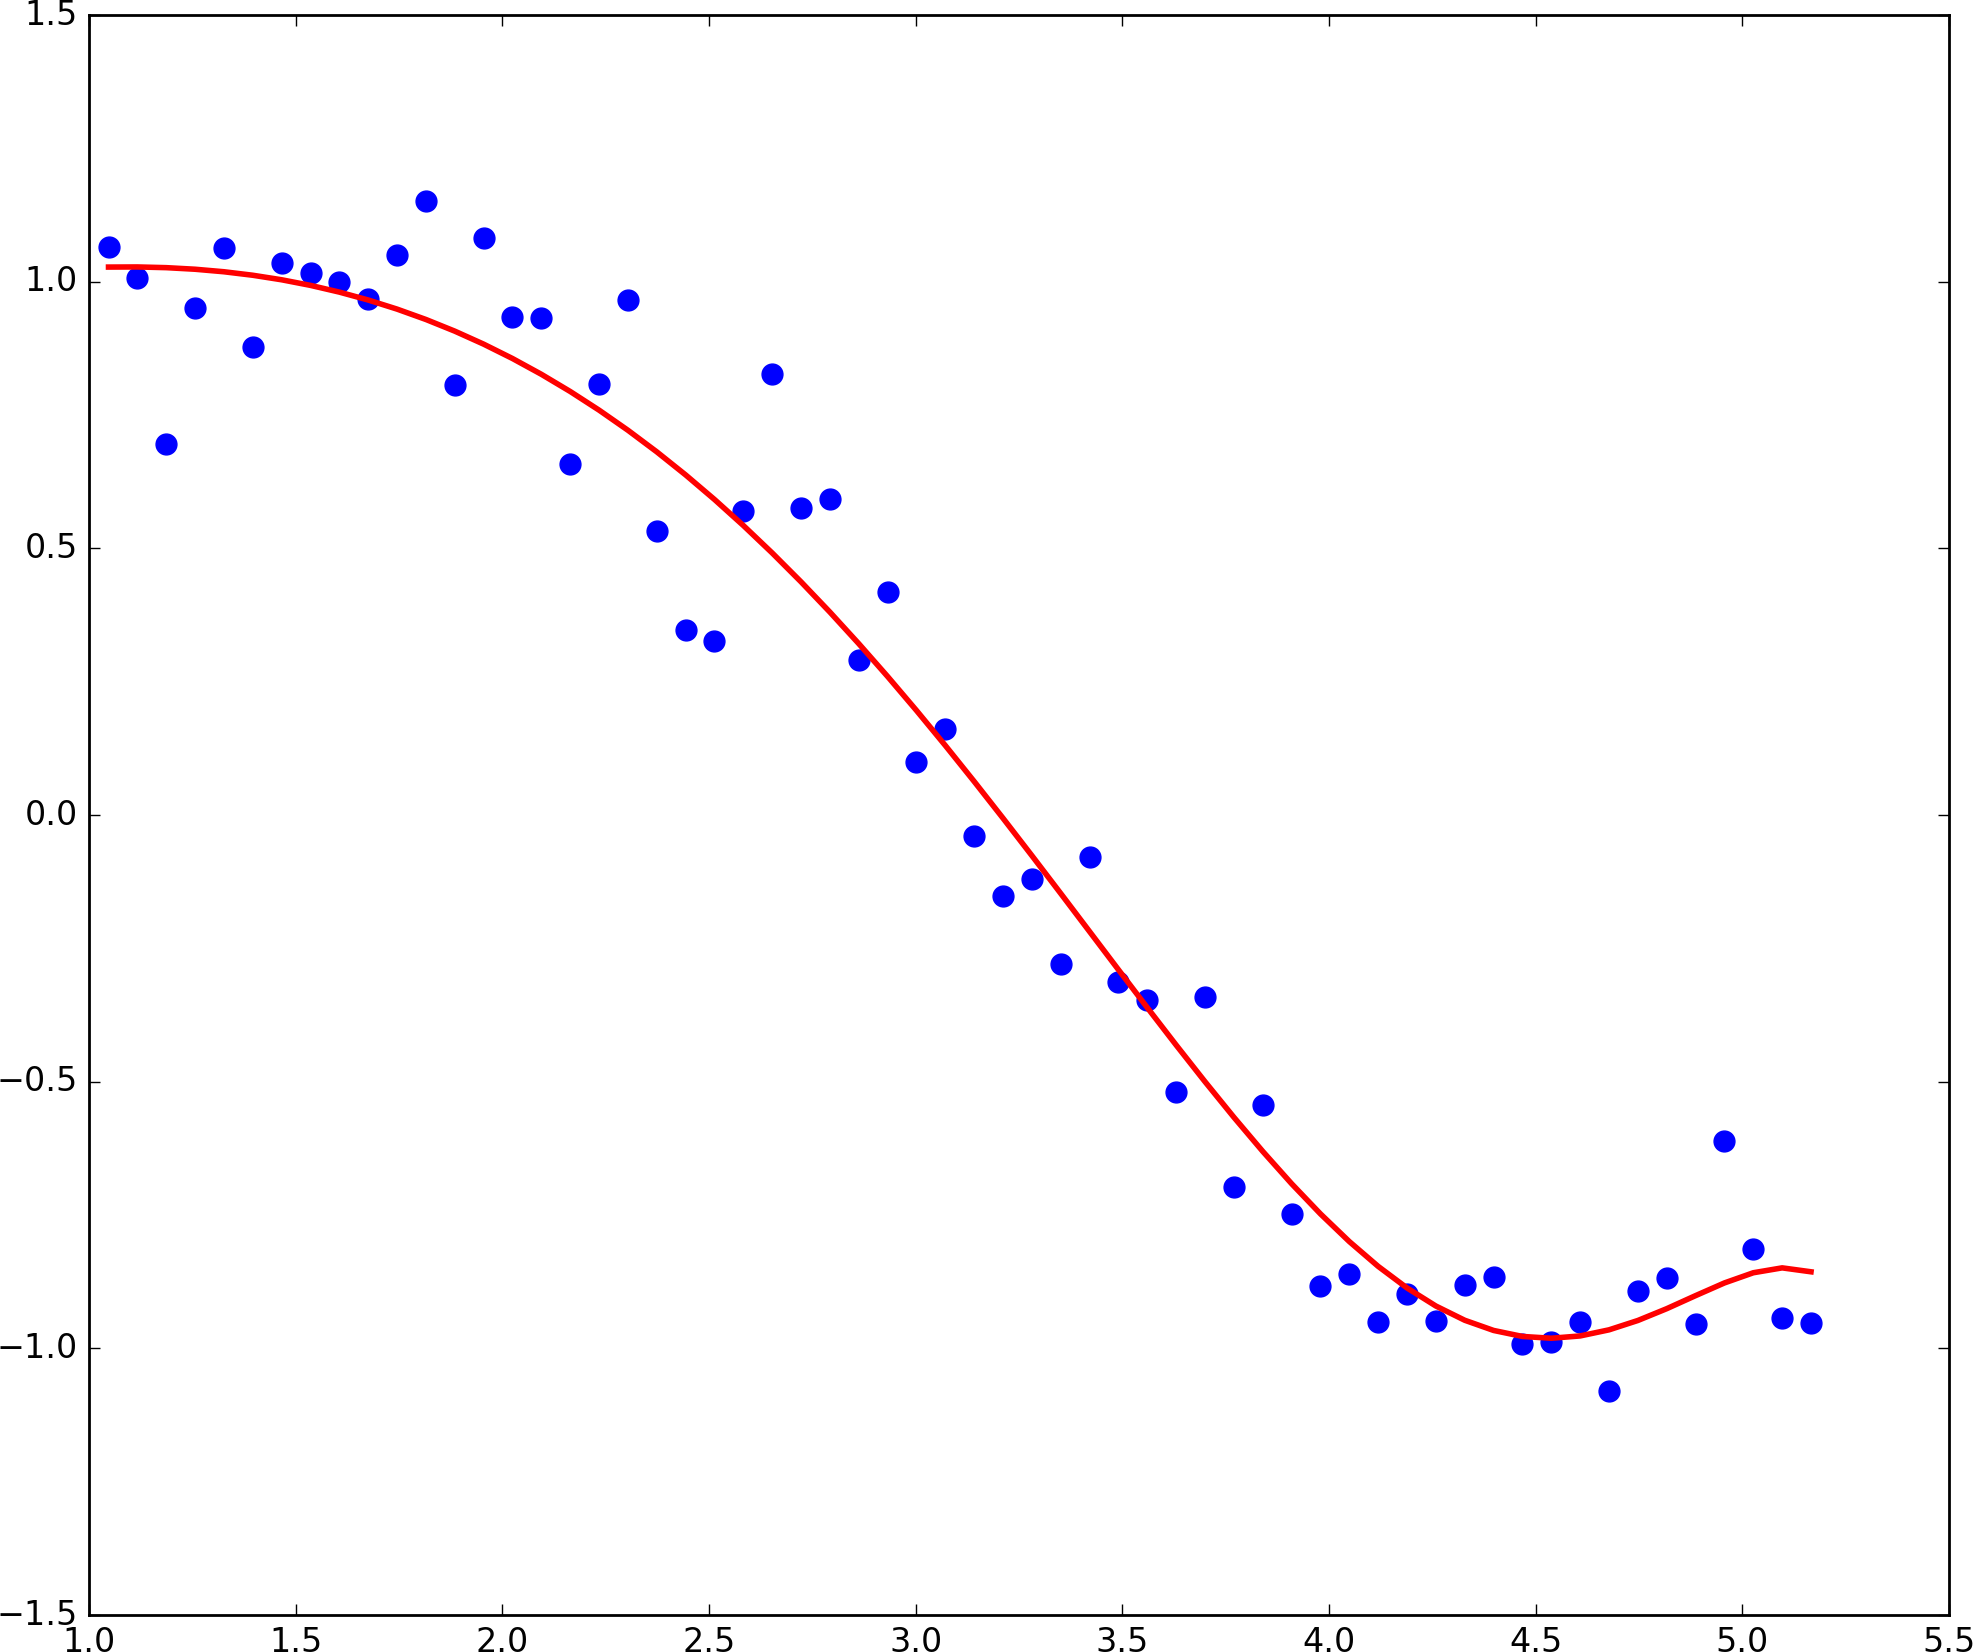
\includegraphics[width=0.99\textwidth]{./lasso_alpha1e-4.png}
\end{figure}
\vspace{-2em}
\begin{figure}
$\alpha=5$
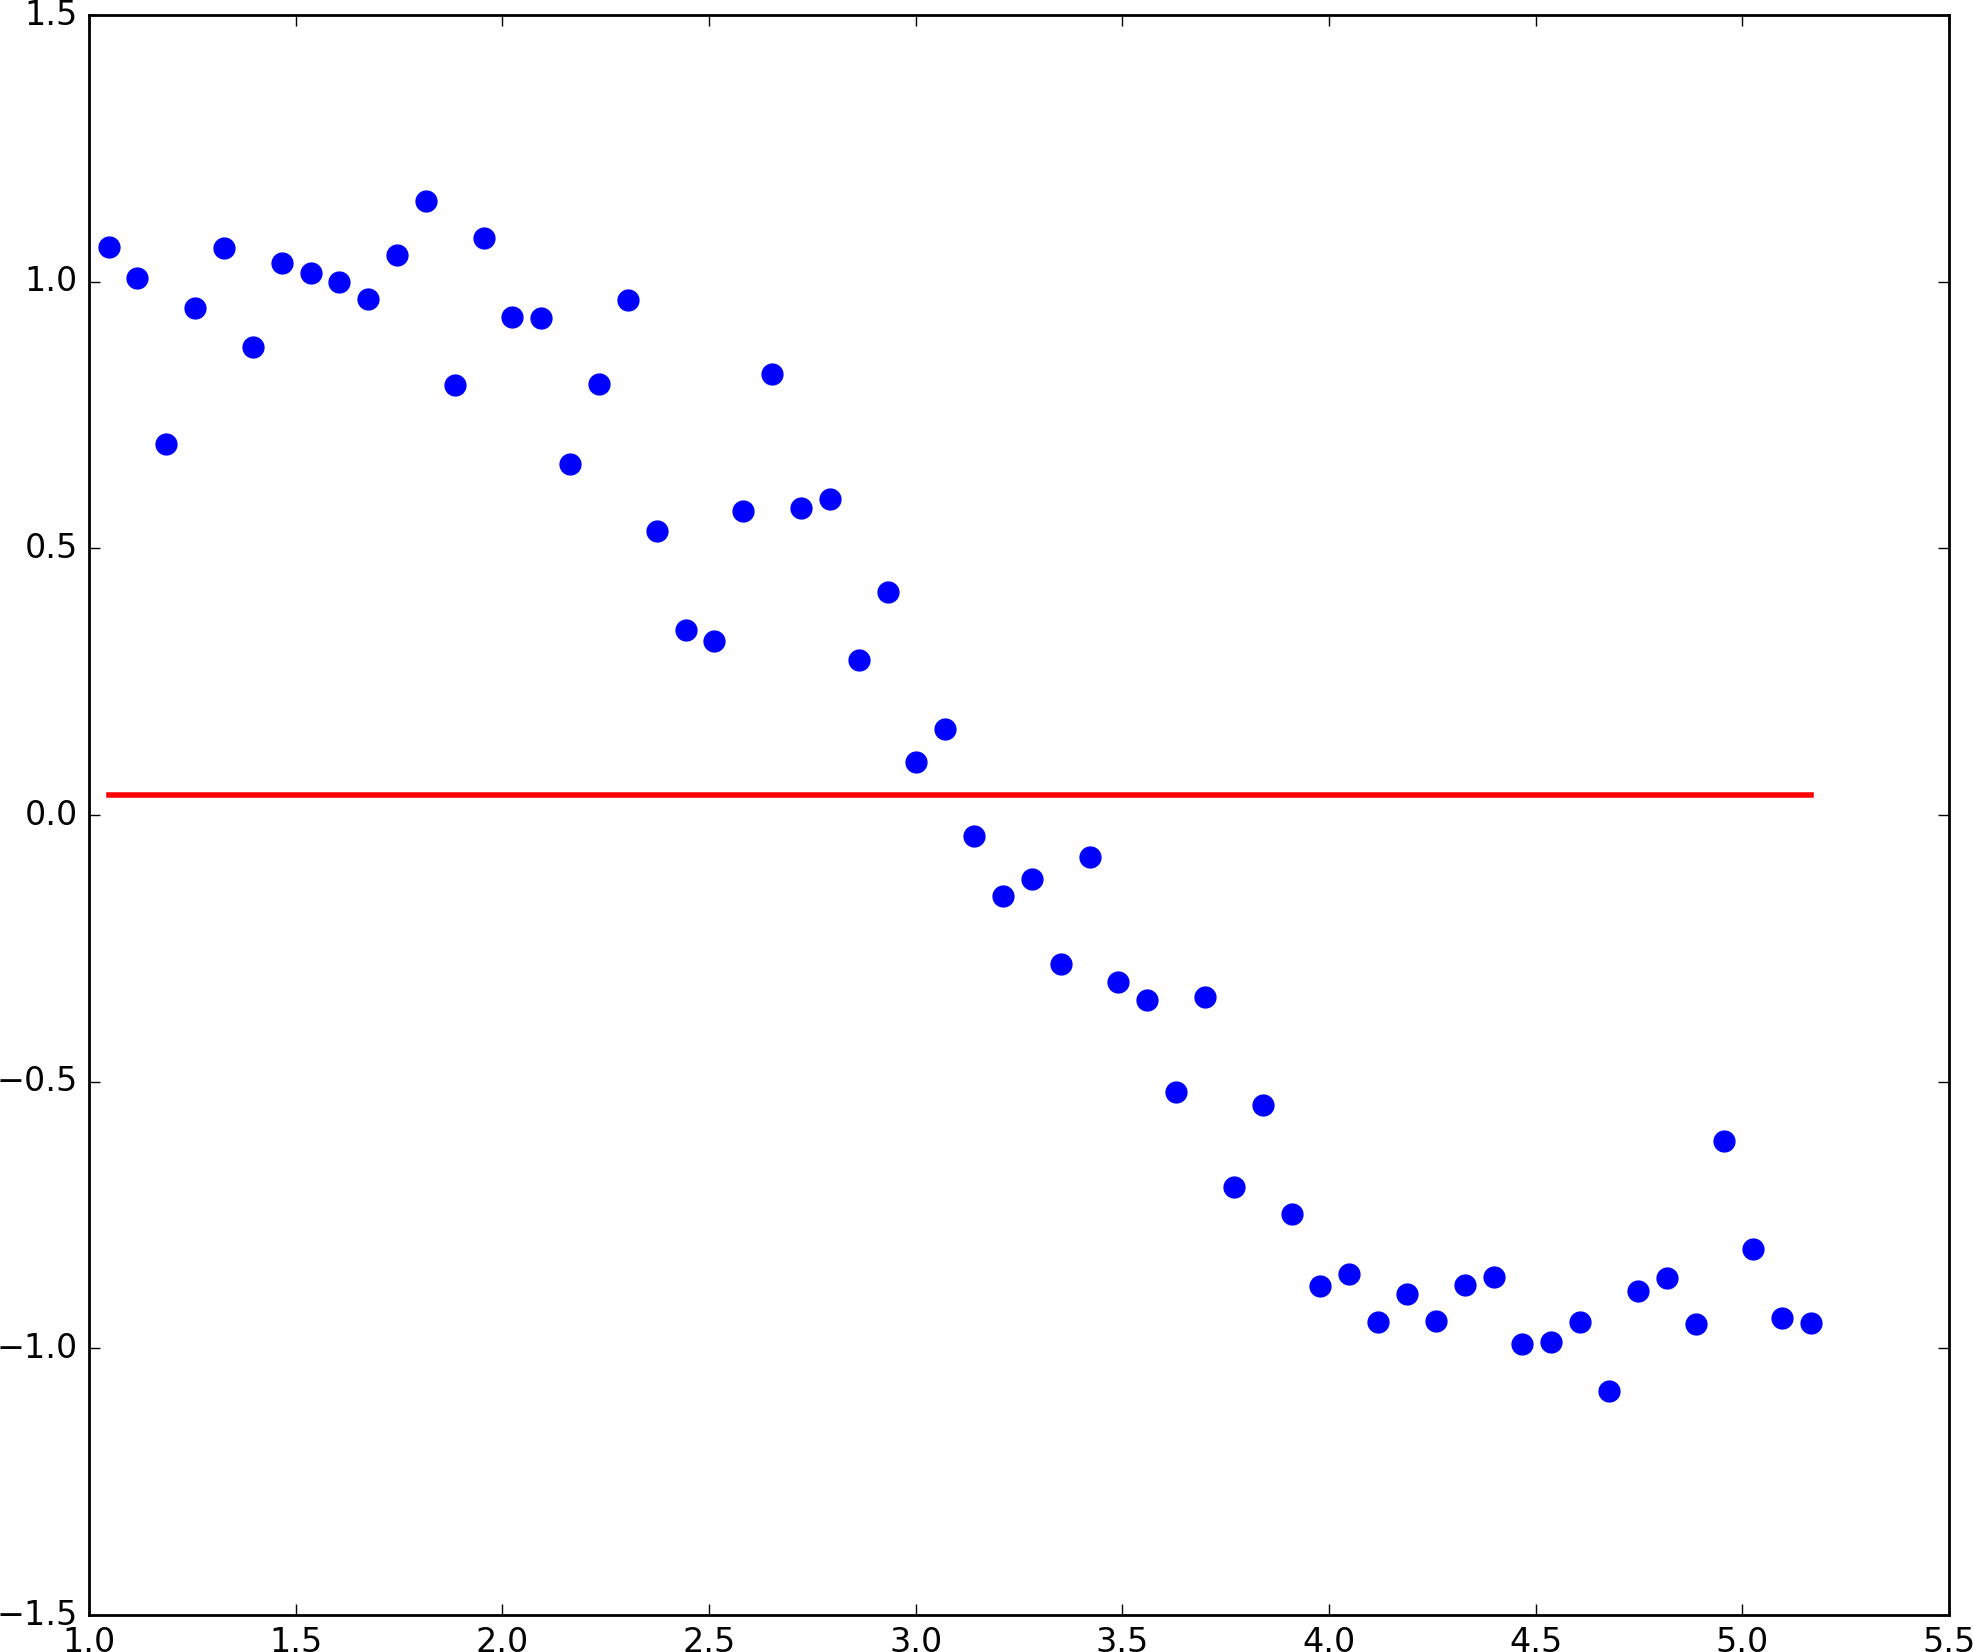
\includegraphics[width=0.99\textwidth]{./lasso_alpha5.png}
\end{figure}
\end{columns}
\end{frame}

%%%%%%%%%%%%%%%%%%%%%
\begin{frame}
\frametitle{Values of coefficients}
\vspace{-2em}
\begin{table}
\resizebox{\textwidth}{!}{%
\begin{tabular}{lllllllllll}
\toprule
{} &      rmse &      th\_0 &      th\_1 &      th\_2 &      th\_3 &      th\_4 &      th\_5 &      th\_6 &      th\_7 &      th\_8 \\
\midrule
alpha\_0      & +1.17e-02 & -3.62e+04 & +2.44e+05 & -7.46e+05 & +1.38e+06 & -1.71e+06 & +1.53e+06 & -1.00e+06 & +4.98e+05 & -1.88e+05 \\
alpha\_1e-15  & +1.59e-02 & +2.22e-01 & +1.06e+00 & -3.69e-01 & +8.85e-04 & +1.63e-03 & -1.19e-04 & -6.44e-05 & -6.28e-06 & +1.45e-06 \\
alpha\_1e-10  & +1.59e-02 & +2.22e-01 & +1.06e+00 & -3.69e-01 & +8.84e-04 & +1.63e-03 & -1.18e-04 & -6.44e-05 & -6.28e-06 & +1.45e-06 \\
alpha\_1e-08  & +1.59e-02 & +2.22e-01 & +1.06e+00 & -3.69e-01 & +7.69e-04 & +1.62e-03 & -1.10e-04 & -6.45e-05 & -6.32e-06 & +1.43e-06 \\
alpha\_0.0001 & +1.72e-02 & +9.03e-01 & +1.71e-01 & -0.00e+00 & -4.78e-02 & -0.00e+00 & -0.00e+00 & +0.00e+00 & +0.00e+00 & +9.47e-06 \\
alpha\_0.001  & +2.80e-02 & +1.29e+00 & -0.00e+00 & -1.26e-01 & -0.00e+00 & -0.00e+00 & -0.00e+00 & +0.00e+00 & +0.00e+00 & +0.00e+00 \\
alpha\_0.01   & +6.07e-02 & +1.76e+00 & -5.52e-01 & -5.62e-04 & -0.00e+00 & -0.00e+00 & -0.00e+00 & -0.00e+00 & -0.00e+00 & -0.00e+00 \\
alpha\_1      & +6.16e-01 & +3.80e-02 & -0.00e+00 & -0.00e+00 & -0.00e+00 & -0.00e+00 & -0.00e+00 & -0.00e+00 & -0.00e+00 & -0.00e+00 \\
alpha\_5      & +6.16e-01 & +3.80e-02 & -0.00e+00 & -0.00e+00 & -0.00e+00 & -0.00e+00 & -0.00e+00 & -0.00e+00 & -0.00e+00 & -0.00e+00 \\
alpha\_10     & +6.16e-01 & +3.80e-02 & -0.00e+00 & -0.00e+00 & -0.00e+00 & -0.00e+00 & -0.00e+00 & -0.00e+00 & -0.00e+00 & -0.00e+00 \\
alpha\_20     & +6.16e-01 & +3.80e-02 & -0.00e+00 & -0.00e+00 & -0.00e+00 & -0.00e+00 & -0.00e+00 & -0.00e+00 & -0.00e+00 & -0.00e+00 \\
\bottomrule
\end{tabular}
}
\end{table}
\begin{figure}
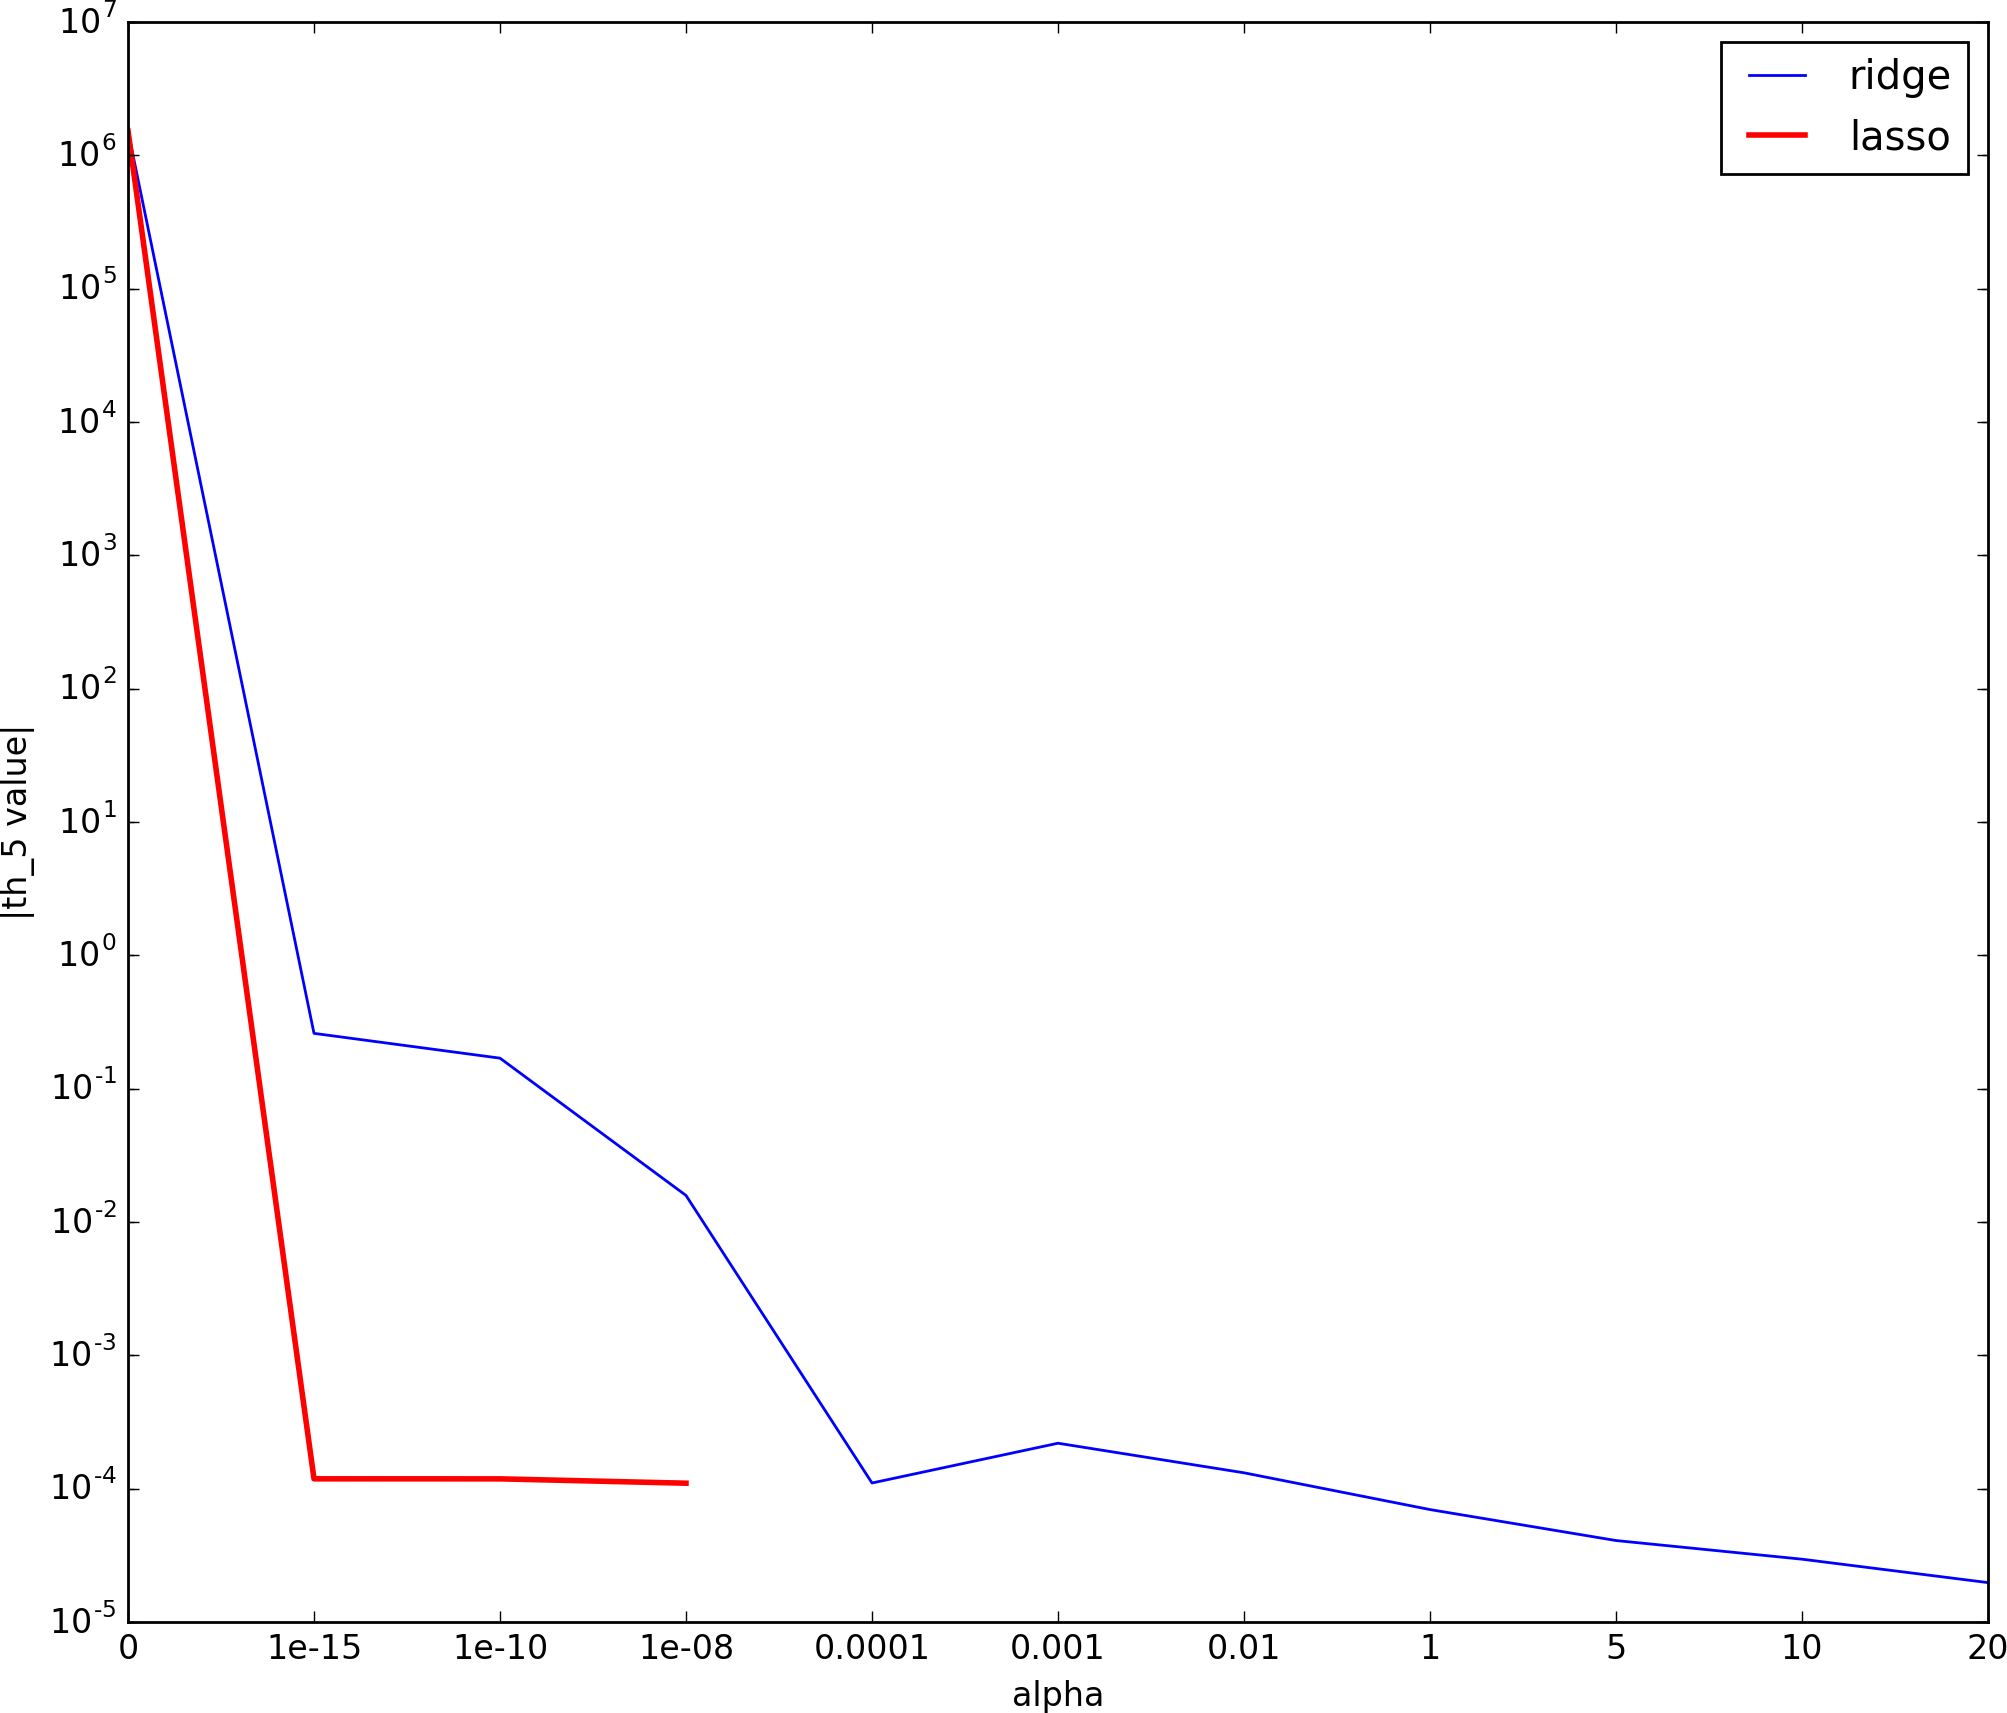
\includegraphics[height=0.4\textheight]{./coefs_th5_lasso.png}\\
Value of $\theta_5$
\end{figure}
\end{frame}

%%%%%%%%%%%%%%%%%%%%
\begin{frame}
\frametitle{Determination of the parameters in the lasso regression}
Considering the cost function J:
$$
J(\bm{\theta}) =J_{lms}(\bm{\theta}) + \alpha \sum_{i=0}^p |\theta_i|
$$
In a gradient algorithm, update of the parameters would be:

J is not differentiable.
If we consider $\theta_{lms} = \theta_i^k -\nu.\frac{\partial J_{lms}}{D\theta_i} $

The update rule is:
\begin{itemize}
\item $\theta_i^{k+1} = \theta_{lms} + \alpha \nu$  if $\theta_{lms} < -\alpha \nu$
\item $\theta_i^k = 0$ if $-\alpha \nu < \theta_{lms} < \alpha \nu$
\item $\theta_i^{k+1} = \theta_{lms} - \alpha \nu$  if $\theta_{lms} > \alpha \nu$
\end{itemize}
\end{frame}

%%%%%%%%%%%%%%%%%%%%
\begin{frame}
\frametitle{Summary of parameters updates}
\begin{figure}
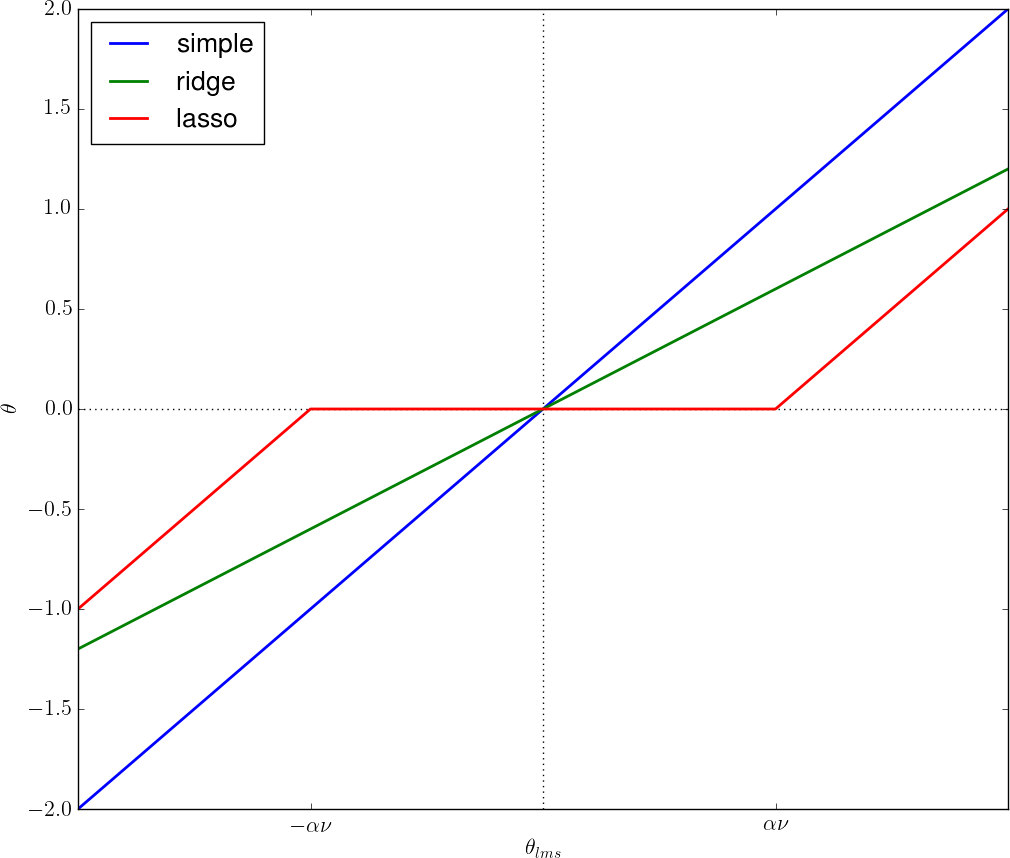
\includegraphics[height=0.8\textheight]{./updates.png}
\end{figure}
\end{frame}

%%%%%%%%%%%%%%%%%%%%%
\begin{frame}
\frametitle{Comparison Ridge/Lasso}
\begin{exampleblock}{Ridge (L2)}
\begin{itemize}
\item Prevents the overfitting
\item includes all the features (dimensions) of the predictor, 
so it can be useless for high dimensional predictors
\end{itemize}
\end{exampleblock}
\pause
\begin{alertblock}{Lasso (L1)}
\begin{itemize}
\item Provides sparse solutions and reduce the dimension of the
predictor
\item If some features in the predictor are correlated, arbitrarily select
one from the others.
\end{itemize}
\end{alertblock}
\end{frame}


\section{Steps of a machine learning process}

%%%%%%%%%%%%%%%%
\begin{frame}{Steps}
    \begin{figure}
        \centering
     \tikzstyle{block} = [rectangle, draw, fill=blue!20, text width=7em, text centered, rounded corners, minimum height=4em]
     \tikzstyle{line} = [draw, ->]
    \tikzstyle{back} = [draw, ->, very thick, red]
     
     \begin{tikzpicture}[auto, node distance=1cm and 2cm]
     \node[block] (collect) {Collect data} ;
     
     \pause
     \node [block, below= of collect] (feature) {Preprocess /clean data\\\footnotesize{\textit{feature extractions}}};
     \path [line] (collect)--(feature);

     \pause
     \node  [block, right= of collect] (tune) {Design model};
     
     \pause
     \node  [block, right= of feature] (train) {Train model};
     \path  [line] (feature)-- node[above]{train} (train);
     \path  [line] (tune)-- (train);
     
     \pause
     \node  [block, below= of train] (evaluate) {Evaluate model};
     \path  [line] (train)--(evaluate);
     \path  [line]  (feature) --  node[above,sloped]{(cross-)valid}(evaluate);

     \pause
     \path  [back]  (evaluate) edge[bend right=80] (tune);
     \path  [back]  (evaluate) edge[bend left] (feature);
     \path  [back]  (evaluate) edge[bend right] (collect);
     
     \pause
     \node  [block, fill=red!20, left=of evaluate]  (release) {Release model};
     \path  [line]  (evaluate)--(release);
     \path  [line]  (feature) -- node[above,sloped]{test} (release);

    

     \end{tikzpicture}
    \end{figure}
\end{frame}

%%%%%%%%%%%%%%%%%%%%%%%%%%%%%%%%%%%%%%%%%%
\begin{frame}{In summary}
    From one dataset, 3 sub-datasets have to be extracted:
    \begin{itemize}
        \item A training dataset
        \item A validation dataset
    \end{itemize}
    Can be done iteratively in a cross-validation procedure.\\
    \alert {Some parameters of the model (e.g. polynomial order in a polynomial regression) were determined from the validation dataset.}
    \begin{itemize}
        \item A test dataset (independent from the two other) to estimate the final performance of the model.
    \end{itemize}
\end{frame}




\end{document}